\documentclass[fleqn,usenatbib]{mnras}

\usepackage{newtxtext,newtxmath}
\usepackage[T1]{fontenc}
\usepackage{ae,aecompl}
%\usepackage{txfonts}
\usepackage{times}

\usepackage{rotating,graphicx}	% Including figure files
\usepackage{amsmath}	% Advanced maths commands
%\usepackage{amssymb}	% Extra maths symbols
\usepackage{ulem}
\usepackage[ampersand]{easylist}

\usepackage{latexsym}
\usepackage{enumerate}% http://ctan.org/pkg/enumerate
\usepackage{amstext}
\usepackage{morefloats}

\usepackage{natbib}
\usepackage{rotating}
\usepackage{changepage}% http://ctan.org/pkg/changepage
\usepackage{scrextend}
\usepackage[ampersand]{easylist}
\usepackage{xcolor}
\usepackage{ulem}

\newcommand{\rt}[1]{{\textcolor{red}{{#1}}}}
\newcommand{\bt}[1]{{\textcolor{blue}{{#1}}}}
\newcommand{\rtc}[1]{{\textcolor{red}{({#1})}}}
\newcommand{\gt}[1]{{\textcolor{}{{#1}}}}
\newcommand{\gtb}[1]{{\textcolor{olive}{[{#1}]}}}
\newcommand{\err}[1]{{\textcolor{cyan}{[{ERR: #1}]}}}
\usepackage{mathtools}
%\usepackage{hyperref}

 
\title[Star Cluster Stellar Wind Retention \& Expulsion]{Should I Stay or Should I Go:  Stellar Wind Retention and Expulsion in Massive Star Clusters}


\author[J.~P.~Naiman et al.]{J.~P.~Naiman$^{1}$\thanks{E-mail: jill.naiman@cfa.harvard.edu}, E.~Ramirez-Ruiz$^{2}$, D.~N.~C.~Lin$^{2}$ 
\vspace*{0.2cm} \\
% List of institutions
$^{1}$Harvard-Smithsonian Center for Astrophysics, 60 Garden Street, Cambridge, MA, 02138, USA\\
  $^2$Department of Astronomy and Astrophysics, University of California, Santa Cruz, CA 95064, USA
}

\date{11 July 2017}

% Enter the current year, for the copyright statements etc.
\pubyear{2017}

% Don't change these lines
\usepackage{tikz}
\usetikzlibrary{tikzmark}

\usepackage{atbegshi,ifthen,listings}
\tikzstyle{highlighter} = [yellow,line width = \baselineskip,]
% from: https://tex.stackexchange.com/questions/15237/highlight-text-in-code-listing-while-also-keeping-syntax-highlighting/49309#49309
\newcounter{highlight}[page]
\newcommand{\tikzhighlightanchor}[1]{\ensuremath{\vcenter{\hbox{\tikz[remember picture, overlay]{\coordinate (#1 highlight \arabic{highlight});}}}}}
\newcommand{\bh}[0]{\stepcounter{highlight}\tikzhighlightanchor{begin}}
\newcommand{\eh}[0]{\tikzhighlightanchor{end}}
\AtBeginShipout{\AtBeginShipoutUpperLeft{\ifthenelse{\value{highlight} > 0}{\tikz[remember picture, overlay]{\foreach \stroke in {1,...,\arabic{highlight}} \draw[highlighter] (begin highlight \stroke) -- (end highlight \stroke);}}{}}}

\begin{document}

\label{firstpage}
\pagerange{\pageref{firstpage}--\pageref{lastpage}}
\maketitle



\begin{abstract}
Mass and energy injection throughout the lifetime of a star cluster contributes to the gas reservoir available for subsequent episodes of star formation and the feedback energy budget responsible for ejecting material from the cluster.
In addition, mass processed in stellar interiors and ejected as winds has the potential to augment the abundance ratios of currently forming stars, or stars which form at a later time from a retained gas reservoir.
Here we present hydrodynamical simulations that explore a wide range of cluster masses, compactnesses, metallicities and stellar population age combinations in order to determine the range of parameter space conducive to stellar wind retention or wind powered gas expulsion in star clusters.
We discuss the effects of the stellar wind prescription on retention and expulsion effectiveness, using MESA stellar evolutionary models as a test bed for exploring how the amounts of wind retention/expulsion depend upon the amount of mixing between the winds from stars of different masses and ages.
We conclude by summarizing some implications for gas retention and expulsion in a variety of compact ($\sigma_v \gtrsim 20 \, {\rm km s^{-1}}$) star clusters including young massive star clusters ($10^5 \lesssim M/M_\odot \lesssim 10^7$, $age \lesssim 500$~Myrs), intermediate age clusters ($10^5 \lesssim M/M_\odot \lesssim 10^7$, $age \approx 1-4$~Gyrs), and globular clusters ($10^5 \lesssim M/M_\odot \lesssim 10^7$, $age \gtrsim 10$~Gyrs).
\end{abstract}

% Select between one and six entries from the list of approved keywords.
% Don't make up new ones.
\begin{keywords}
galaxies: star clusters: general -- stars: mass-loss -- (Galaxy:) globular clusters: general\end{keywords}

%%%%%%%%%%%%%%%%%%%%%%%%%%%%%%%%%%%%%%%%%%%%%%%%%%



\section{Introduction}
 

 \tikzmark{mainBodyStart0}Whether\tikzmark{mainBodyEnd0} \tikzmark{mainBodyStart1}and\tikzmark{mainBodyEnd1} \tikzmark{mainBodyStart2}when\tikzmark{mainBodyEnd2} \tikzmark{mainBodyStart3}gas\tikzmark{mainBodyEnd3} \tikzmark{mainBodyStart4}is\tikzmark{mainBodyEnd4} \tikzmark{mainBodyStart5}retained\tikzmark{mainBodyEnd5} \tikzmark{mainBodyStart6}within\tikzmark{mainBodyEnd6} \tikzmark{mainBodyStart7}a\tikzmark{mainBodyEnd7} \tikzmark{mainBodyStart8}star\tikzmark{mainBodyEnd8} \tikzmark{mainBodyStart9}cluster,\tikzmark{mainBodyEnd9} \tikzmark{mainBodyStart10}along\tikzmark{mainBodyEnd10} \tikzmark{mainBodyStart11}with\tikzmark{mainBodyEnd11} \tikzmark{mainBodyStart12}inter-cluster\tikzmark{mainBodyEnd12} \tikzmark{mainBodyStart13}and\tikzmark{mainBodyEnd13} \tikzmark{mainBodyStart14}intra-cluster\tikzmark{mainBodyEnd14} \tikzmark{mainBodyStart15}gas\tikzmark{mainBodyEnd15} \tikzmark{mainBodyStart16}heating\tikzmark{mainBodyEnd16} \tikzmark{mainBodyStart17}mechanisms\tikzmark{mainBodyEnd17} \tikzmark{mainBodyStart18}determines\tikzmark{mainBodyEnd18} \tikzmark{mainBodyStart19}the\tikzmark{mainBodyEnd19} \tikzmark{mainBodyStart20}star\tikzmark{mainBodyEnd20} \tikzmark{mainBodyStart21}formation\tikzmark{mainBodyEnd21} \tikzmark{mainBodyStart22}history\tikzmark{mainBodyEnd22} \tikzmark{mainBodyStart23}of\tikzmark{mainBodyEnd23} \tikzmark{mainBodyStart24}the\tikzmark{mainBodyEnd24} \tikzmark{mainBodyStart25}cluster.\tikzmark{mainBodyEnd25}
 \tikzmark{mainBodyStart26}Many\tikzmark{mainBodyEnd26} \tikzmark{mainBodyStart27}cluster\tikzmark{mainBodyEnd27} \tikzmark{mainBodyStart28}properties\tikzmark{mainBodyEnd28} \tikzmark{mainBodyStart29}can\tikzmark{mainBodyEnd29} \tikzmark{mainBodyStart30}be\tikzmark{mainBodyEnd30} \tikzmark{mainBodyStart31}responsible\tikzmark{mainBodyEnd31} \tikzmark{mainBodyStart32}for\tikzmark{mainBodyEnd32} \tikzmark{mainBodyStart33}gas\tikzmark{mainBodyEnd33} \tikzmark{mainBodyStart34}retention\tikzmark{mainBodyEnd34} \tikzmark{mainBodyStart35}or\tikzmark{mainBodyEnd35} \tikzmark{mainBodyStart36}expulsion\tikzmark{mainBodyEnd36} \tikzmark{mainBodyStart37}in\tikzmark{mainBodyEnd37} \tikzmark{mainBodyStart38}a\tikzmark{mainBodyEnd38} \tikzmark{mainBodyStart39}cluster\tikzmark{mainBodyEnd39} \tikzmark{mainBodyStart40}-\tikzmark{mainBodyEnd40} \tikzmark{mainBodyStart41}the\tikzmark{mainBodyEnd41} \tikzmark{mainBodyStart42}cluster's\tikzmark{mainBodyEnd42} \tikzmark{mainBodyStart43}compactness,\tikzmark{mainBodyEnd43} \tikzmark{mainBodyStart44}cluster\tikzmark{mainBodyEnd44} \tikzmark{mainBodyStart45}mass,\tikzmark{mainBodyEnd45} \tikzmark{mainBodyStart46}ability\tikzmark{mainBodyEnd46} \tikzmark{mainBodyStart47}to\tikzmark{mainBodyEnd47} \tikzmark{mainBodyStart48}cool\tikzmark{mainBodyEnd48} \tikzmark{mainBodyStart49}effectively,\tikzmark{mainBodyEnd49} \tikzmark{mainBodyStart50}mass\tikzmark{mainBodyEnd50} \tikzmark{mainBodyStart51}and\tikzmark{mainBodyEnd51} \tikzmark{mainBodyStart52}temperature\tikzmark{mainBodyEnd52} \tikzmark{mainBodyStart53}of\tikzmark{mainBodyEnd53} \tikzmark{mainBodyStart54}gas\tikzmark{mainBodyEnd54} \tikzmark{mainBodyStart55}reservoir,\tikzmark{mainBodyEnd55} \tikzmark{mainBodyStart56}and\tikzmark{mainBodyEnd56} \tikzmark{mainBodyStart57}efficiency\tikzmark{mainBodyEnd57} \tikzmark{mainBodyStart58}of\tikzmark{mainBodyEnd58} \tikzmark{mainBodyStart59}internal\tikzmark{mainBodyEnd59} \tikzmark{mainBodyStart60}and\tikzmark{mainBodyEnd60} \tikzmark{mainBodyStart61}external\tikzmark{mainBodyEnd61} \tikzmark{mainBodyStart62}heating\tikzmark{mainBodyEnd62} \tikzmark{mainBodyStart63}mechanisms.\tikzmark{mainBodyEnd63}  
 \tikzmark{mainBodyStart64}As\tikzmark{mainBodyEnd64} \tikzmark{mainBodyStart65}it\tikzmark{mainBodyEnd65} \tikzmark{mainBodyStart66}thought\tikzmark{mainBodyEnd66} \tikzmark{mainBodyStart67}that\tikzmark{mainBodyEnd67} \tikzmark{mainBodyStart68}most\tikzmark{mainBodyEnd68} \tikzmark{mainBodyStart69}stars\tikzmark{mainBodyEnd69} \tikzmark{mainBodyStart70}form\tikzmark{mainBodyEnd70} \tikzmark{mainBodyStart71}in\tikzmark{mainBodyEnd71} \tikzmark{mainBodyStart72}clusters\tikzmark{mainBodyEnd72} \citep[e.g.][]{lada2003} \tikzmark{mainBodyStart73}the\tikzmark{mainBodyEnd73} \tikzmark{mainBodyStart74}study\tikzmark{mainBodyEnd74} \tikzmark{mainBodyStart75}of\tikzmark{mainBodyEnd75} \tikzmark{mainBodyStart76}which\tikzmark{mainBodyEnd76} \tikzmark{mainBodyStart77}parameters\tikzmark{mainBodyEnd77} \tikzmark{mainBodyStart78}and\tikzmark{mainBodyEnd78} \tikzmark{mainBodyStart79}mechanisms\tikzmark{mainBodyEnd79} \tikzmark{mainBodyStart80}are\tikzmark{mainBodyEnd80} \tikzmark{mainBodyStart81}important\tikzmark{mainBodyEnd81} \tikzmark{mainBodyStart82}at\tikzmark{mainBodyEnd82} \tikzmark{mainBodyStart83}different\tikzmark{mainBodyEnd83} \tikzmark{mainBodyStart84}cluster\tikzmark{mainBodyEnd84} \tikzmark{mainBodyStart85}evolutionary\tikzmark{mainBodyEnd85} \tikzmark{mainBodyStart86}times\tikzmark{mainBodyEnd86} \tikzmark{mainBodyStart87}is\tikzmark{mainBodyEnd87} \tikzmark{mainBodyStart88}crucial\tikzmark{mainBodyEnd88} \tikzmark{mainBodyStart89}to\tikzmark{mainBodyEnd89} \tikzmark{mainBodyStart90}understand\tikzmark{mainBodyEnd90} \tikzmark{mainBodyStart91}when\tikzmark{mainBodyEnd91} \tikzmark{mainBodyStart92}favorable\tikzmark{mainBodyEnd92} \tikzmark{mainBodyStart93}conditions\tikzmark{mainBodyEnd93} \tikzmark{mainBodyStart94}for\tikzmark{mainBodyEnd94} \tikzmark{mainBodyStart95}star\tikzmark{mainBodyEnd95} \tikzmark{mainBodyStart96}formation\tikzmark{mainBodyEnd96} \tikzmark{mainBodyStart97}arise\tikzmark{mainBodyEnd97} \tikzmark{mainBodyStart98}throughout\tikzmark{mainBodyEnd98} \tikzmark{mainBodyStart99}a\tikzmark{mainBodyEnd99} \tikzmark{mainBodyStart100}cluster's\tikzmark{mainBodyEnd100} \tikzmark{mainBodyStart101}lifetime.\tikzmark{mainBodyEnd101}

 \tikzmark{mainBodyStart102}Observations\tikzmark{mainBodyEnd102} \tikzmark{mainBodyStart103}of\tikzmark{mainBodyEnd103} \tikzmark{mainBodyStart104}young\tikzmark{mainBodyEnd104} \tikzmark{mainBodyStart105}massive\tikzmark{mainBodyEnd105} \tikzmark{mainBodyStart106}clusters\tikzmark{mainBodyEnd106} \tikzmark{mainBodyStart107}(YMCs),\tikzmark{mainBodyEnd107} \tikzmark{mainBodyStart108}intermediate\tikzmark{mainBodyEnd108} \tikzmark{mainBodyStart109}age\tikzmark{mainBodyEnd109} \tikzmark{mainBodyStart110}clusters\tikzmark{mainBodyEnd110} \tikzmark{mainBodyStart111}(IACs)\tikzmark{mainBodyEnd111} \tikzmark{mainBodyStart112}and\tikzmark{mainBodyEnd112} \tikzmark{mainBodyStart113}globular\tikzmark{mainBodyEnd113} \tikzmark{mainBodyStart114}clusters\tikzmark{mainBodyEnd114} \tikzmark{mainBodyStart115}(GCs)\tikzmark{mainBodyEnd115} \tikzmark{mainBodyStart116}potentially\tikzmark{mainBodyEnd116} \tikzmark{mainBodyStart117}give\tikzmark{mainBodyEnd117} \tikzmark{mainBodyStart118}us\tikzmark{mainBodyEnd118} \tikzmark{mainBodyStart119}insights\tikzmark{mainBodyEnd119} \tikzmark{mainBodyStart120}into\tikzmark{mainBodyEnd120} \tikzmark{mainBodyStart121}gas\tikzmark{mainBodyEnd121} \tikzmark{mainBodyStart122}retention\tikzmark{mainBodyEnd122} \tikzmark{mainBodyStart123}at\tikzmark{mainBodyEnd123} \tikzmark{mainBodyStart124}different\tikzmark{mainBodyEnd124} \tikzmark{mainBodyStart125}times\tikzmark{mainBodyEnd125} \tikzmark{mainBodyStart126}within\tikzmark{mainBodyEnd126} \tikzmark{mainBodyStart127}massive\tikzmark{mainBodyEnd127} \tikzmark{mainBodyStart128}star\tikzmark{mainBodyEnd128} \tikzmark{mainBodyStart129}clusters\tikzmark{mainBodyEnd129} \citep[e.g.][]{bastian2017}
 \tikzmark{mainBodyStart130}Additionally,\tikzmark{mainBodyEnd130} \tikzmark{mainBodyStart131}if\tikzmark{mainBodyEnd131} \tikzmark{mainBodyStart132}GCs\tikzmark{mainBodyEnd132} \tikzmark{mainBodyStart133}evolve\tikzmark{mainBodyEnd133} \tikzmark{mainBodyStart134}from\tikzmark{mainBodyEnd134} \tikzmark{mainBodyStart135}YMCs\tikzmark{mainBodyEnd135} \tikzmark{mainBodyStart136}and\tikzmark{mainBodyEnd136} \tikzmark{mainBodyStart137}IACs\tikzmark{mainBodyEnd137} \tikzmark{mainBodyStart138}as\tikzmark{mainBodyEnd138} \tikzmark{mainBodyStart139}some\tikzmark{mainBodyEnd139} \tikzmark{mainBodyStart140}have\tikzmark{mainBodyEnd140} \tikzmark{mainBodyStart141}suggested\tikzmark{mainBodyEnd141} \citep{longmore2014,krui2015} \tikzmark{mainBodyStart142}then\tikzmark{mainBodyEnd142} \tikzmark{mainBodyStart143}observations\tikzmark{mainBodyEnd143} \tikzmark{mainBodyStart144}of\tikzmark{mainBodyEnd144} \tikzmark{mainBodyStart145}each\tikzmark{mainBodyEnd145} \tikzmark{mainBodyStart146}type\tikzmark{mainBodyEnd146} \tikzmark{mainBodyStart147}of\tikzmark{mainBodyEnd147} \tikzmark{mainBodyStart148}system\tikzmark{mainBodyEnd148} \tikzmark{mainBodyStart149}provides\tikzmark{mainBodyEnd149} \tikzmark{mainBodyStart150}clues\tikzmark{mainBodyEnd150} \tikzmark{mainBodyStart151}to\tikzmark{mainBodyEnd151} \tikzmark{mainBodyStart152}the\tikzmark{mainBodyEnd152} \tikzmark{mainBodyStart153}origin\tikzmark{mainBodyEnd153} \tikzmark{mainBodyStart154}of\tikzmark{mainBodyEnd154} \tikzmark{mainBodyStart155}the\tikzmark{mainBodyEnd155} \tikzmark{mainBodyStart156}high\tikzmark{mainBodyEnd156} \tikzmark{mainBodyStart157}level\tikzmark{mainBodyEnd157} \tikzmark{mainBodyStart158}of\tikzmark{mainBodyEnd158} \tikzmark{mainBodyStart159}occurrence\tikzmark{mainBodyEnd159} \tikzmark{mainBodyStart160}of\tikzmark{mainBodyEnd160} \tikzmark{mainBodyStart161}multiple\tikzmark{mainBodyEnd161} \tikzmark{mainBodyStart162}subpopulations\tikzmark{mainBodyEnd162} \tikzmark{mainBodyStart163}with\tikzmark{mainBodyEnd163} \tikzmark{mainBodyStart164}different\tikzmark{mainBodyEnd164} \tikzmark{mainBodyStart165}abundance\tikzmark{mainBodyEnd165} \tikzmark{mainBodyStart166}ratios\tikzmark{mainBodyEnd166} \tikzmark{mainBodyStart167}within\tikzmark{mainBodyEnd167} \tikzmark{mainBodyStart168}present\tikzmark{mainBodyEnd168} \tikzmark{mainBodyStart169}day\tikzmark{mainBodyEnd169} \tikzmark{mainBodyStart170}GCs.\tikzmark{mainBodyEnd170}

 \tikzmark{mainBodyStart171}Variations\tikzmark{mainBodyEnd171} \tikzmark{mainBodyStart172}in\tikzmark{mainBodyEnd172} \tikzmark{mainBodyStart173}the\tikzmark{mainBodyEnd173} \tikzmark{mainBodyStart174}abundances\tikzmark{mainBodyEnd174} \tikzmark{mainBodyStart175}of\tikzmark{mainBodyEnd175} \tikzmark{mainBodyStart176}He,\tikzmark{mainBodyEnd176} \tikzmark{mainBodyStart177}Mg,\tikzmark{mainBodyEnd177} \tikzmark{mainBodyStart178}C,\tikzmark{mainBodyEnd178} \tikzmark{mainBodyStart179}N,\tikzmark{mainBodyEnd179} \tikzmark{mainBodyStart180}O,\tikzmark{mainBodyEnd180} \tikzmark{mainBodyStart181}Mg,\tikzmark{mainBodyEnd181} \tikzmark{mainBodyStart182}Na\tikzmark{mainBodyEnd182} \tikzmark{mainBodyStart183}and\tikzmark{mainBodyEnd183} \tikzmark{mainBodyStart184}Al\tikzmark{mainBodyEnd184} \tikzmark{mainBodyStart185}in\tikzmark{mainBodyEnd185} \tikzmark{mainBodyStart186}main\tikzmark{mainBodyEnd186} \tikzmark{mainBodyStart187}sequence\tikzmark{mainBodyEnd187} \tikzmark{mainBodyStart188}stars\tikzmark{mainBodyEnd188} \citep{gratton2001,briley2002,cohen2002,cannon1998,pancino2010b} \tikzmark{mainBodyStart189}and\tikzmark{mainBodyEnd189} \tikzmark{mainBodyStart190}RGB\tikzmark{mainBodyEnd190} \tikzmark{mainBodyStart191}stars\tikzmark{mainBodyEnd191} \citep{sneden2004} \tikzmark{mainBodyStart192}within\tikzmark{mainBodyEnd192} \tikzmark{mainBodyStart193}the\tikzmark{mainBodyEnd193} \tikzmark{mainBodyStart194}majority\tikzmark{mainBodyEnd194} \tikzmark{mainBodyStart195}of\tikzmark{mainBodyEnd195} \tikzmark{mainBodyStart196}Galactic\tikzmark{mainBodyEnd196} \tikzmark{mainBodyStart197}globular\tikzmark{mainBodyEnd197} \tikzmark{mainBodyStart198}clusters\tikzmark{mainBodyEnd198} \tikzmark{mainBodyStart199}suggest\tikzmark{mainBodyEnd199} \tikzmark{mainBodyStart200}a\tikzmark{mainBodyEnd200} \tikzmark{mainBodyStart201}complex\tikzmark{mainBodyEnd201} \tikzmark{mainBodyStart202}enrichment\tikzmark{mainBodyEnd202} \tikzmark{mainBodyStart203}history\tikzmark{mainBodyEnd203} \tikzmark{mainBodyStart204}during\tikzmark{mainBodyEnd204} \tikzmark{mainBodyStart205}the\tikzmark{mainBodyEnd205} \tikzmark{mainBodyStart206}formation\tikzmark{mainBodyEnd206} \tikzmark{mainBodyStart207}of\tikzmark{mainBodyEnd207} \tikzmark{mainBodyStart208}stars\tikzmark{mainBodyEnd208} \tikzmark{mainBodyStart209}within\tikzmark{mainBodyEnd209} \tikzmark{mainBodyStart210}these\tikzmark{mainBodyEnd210} \tikzmark{mainBodyStart211}systems.\tikzmark{mainBodyEnd211}
 \tikzmark{mainBodyStart212}In\tikzmark{mainBodyEnd212} \tikzmark{mainBodyStart213}addition,\tikzmark{mainBodyEnd213} \tikzmark{mainBodyStart214}the\tikzmark{mainBodyEnd214} \tikzmark{mainBodyStart215}observed\tikzmark{mainBodyEnd215} \tikzmark{mainBodyStart216}anti-correlations\tikzmark{mainBodyEnd216} \tikzmark{mainBodyStart217}between\tikzmark{mainBodyEnd217} \tikzmark{mainBodyStart218}several\tikzmark{mainBodyEnd218} \tikzmark{mainBodyStart219}elements\tikzmark{mainBodyEnd219} \citep[Na-O and Mg-Al;][]{kraft1993,ivans1999,carretta2006b,carretta2009b,conroy2012} \tikzmark{mainBodyStart220}require\tikzmark{mainBodyEnd220} \tikzmark{mainBodyStart221}a\tikzmark{mainBodyEnd221} \tikzmark{mainBodyStart222}significant\tikzmark{mainBodyEnd222} \tikzmark{mainBodyStart223}fraction\tikzmark{mainBodyEnd223} \tikzmark{mainBodyStart224}of\tikzmark{mainBodyEnd224} \tikzmark{mainBodyStart225}the\tikzmark{mainBodyEnd225} \tikzmark{mainBodyStart226}enriching\tikzmark{mainBodyEnd226} \tikzmark{mainBodyStart227}material\tikzmark{mainBodyEnd227} \tikzmark{mainBodyStart228}to\tikzmark{mainBodyEnd228} \tikzmark{mainBodyStart229}be\tikzmark{mainBodyEnd229} \tikzmark{mainBodyStart230}processed\tikzmark{mainBodyEnd230} \tikzmark{mainBodyStart231}at\tikzmark{mainBodyEnd231} \tikzmark{mainBodyStart232}temperatures\tikzmark{mainBodyEnd232} \tikzmark{mainInlineStart233}$> 10^7 \, {\rm K}$\tikzmark{mainInlineEnd233} \tikzmark{mainBodyStart234}in\tikzmark{mainBodyEnd234} \tikzmark{mainBodyStart235}order\tikzmark{mainBodyEnd235} \tikzmark{mainBodyStart236}for\tikzmark{mainBodyEnd236} \tikzmark{mainBodyStart237}the\tikzmark{mainBodyEnd237} \tikzmark{mainBodyStart238}CNO,\tikzmark{mainBodyEnd238} \tikzmark{mainBodyStart239}Na-Ne\tikzmark{mainBodyEnd239} \tikzmark{mainBodyStart240}and\tikzmark{mainBodyEnd240} \tikzmark{mainBodyStart241}Mg-Al\tikzmark{mainBodyEnd241} \tikzmark{mainBodyStart242}cycles\tikzmark{mainBodyEnd242} \tikzmark{mainBodyStart243}to\tikzmark{mainBodyEnd243} \tikzmark{mainBodyStart244}be\tikzmark{mainBodyEnd244} \tikzmark{mainBodyStart245}activated\tikzmark{mainBodyEnd245} \citep{karakas2007,ventura2008b}
 \tikzmark{mainBodyStart246}As\tikzmark{mainBodyEnd246} \tikzmark{mainBodyStart247}the\tikzmark{mainBodyEnd247} \tikzmark{mainBodyStart248}anomalous\tikzmark{mainBodyEnd248} \tikzmark{mainBodyStart249}population\tikzmark{mainBodyEnd249} \tikzmark{mainBodyStart250}is\tikzmark{mainBodyEnd250} \tikzmark{mainBodyStart251}responsible\tikzmark{mainBodyEnd251} \tikzmark{mainBodyStart252}for\tikzmark{mainBodyEnd252} \tikzmark{mainBodyStart253}30-70\tikzmark{mainBodyEnd253} \tikzmark{mainBodyStart254}of\tikzmark{mainBodyEnd254} \tikzmark{mainBodyStart255}the\tikzmark{mainBodyEnd255} \tikzmark{mainBodyStart256}stellar\tikzmark{mainBodyEnd256} \tikzmark{mainBodyStart257}content\tikzmark{mainBodyEnd257} \tikzmark{mainBodyStart258}of\tikzmark{mainBodyEnd258} \tikzmark{mainBodyStart259}the\tikzmark{mainBodyEnd259} \tikzmark{mainBodyStart260}globular\tikzmark{mainBodyEnd260} \tikzmark{mainBodyStart261}clusters\tikzmark{mainBodyEnd261} \citep[e.g.][]{carretta2009} \tikzmark{mainBodyStart262}any\tikzmark{mainBodyEnd262} \tikzmark{mainBodyStart263}scenario\tikzmark{mainBodyEnd263} \tikzmark{mainBodyStart264}invoked\tikzmark{mainBodyEnd264} \tikzmark{mainBodyStart265}to\tikzmark{mainBodyEnd265} \tikzmark{mainBodyStart266}explain\tikzmark{mainBodyEnd266} \tikzmark{mainBodyStart267}this\tikzmark{mainBodyEnd267} \tikzmark{mainBodyStart268}complex\tikzmark{mainBodyEnd268} \tikzmark{mainBodyStart269}star\tikzmark{mainBodyEnd269} \tikzmark{mainBodyStart270}formation\tikzmark{mainBodyEnd270} \tikzmark{mainBodyStart271}history\tikzmark{mainBodyEnd271} \tikzmark{mainBodyStart272}must\tikzmark{mainBodyEnd272} \tikzmark{mainBodyStart273}also\tikzmark{mainBodyEnd273} \tikzmark{mainBodyStart274}account\tikzmark{mainBodyEnd274} \tikzmark{mainBodyStart275}for\tikzmark{mainBodyEnd275} \tikzmark{mainBodyStart276}the\tikzmark{mainBodyEnd276} \tikzmark{mainBodyStart277}pollution\tikzmark{mainBodyEnd277} \tikzmark{mainBodyStart278}of\tikzmark{mainBodyEnd278} \tikzmark{mainBodyStart279}a\tikzmark{mainBodyEnd279} \tikzmark{mainBodyStart280}significant\tikzmark{mainBodyEnd280} \tikzmark{mainBodyStart281}portion\tikzmark{mainBodyEnd281} \tikzmark{mainBodyStart282}of\tikzmark{mainBodyEnd282} \tikzmark{mainBodyStart283}the\tikzmark{mainBodyEnd283} \tikzmark{mainBodyStart284}stellar\tikzmark{mainBodyEnd284} \tikzmark{mainBodyStart285}population\tikzmark{mainBodyEnd285} \tikzmark{mainBodyStart286}or\tikzmark{mainBodyEnd286} \tikzmark{mainBodyStart287}the\tikzmark{mainBodyEnd287} \tikzmark{mainBodyStart288}removal\tikzmark{mainBodyEnd288} \tikzmark{mainBodyStart289}of\tikzmark{mainBodyEnd289} \tikzmark{mainBodyStart290}the\tikzmark{mainBodyEnd290} \tikzmark{mainBodyStart291}majority\tikzmark{mainBodyEnd291} \tikzmark{mainBodyStart292}of\tikzmark{mainBodyEnd292} \tikzmark{mainBodyStart293}the\tikzmark{mainBodyEnd293} \tikzmark{mainBodyStart294}unpolluted\tikzmark{mainBodyEnd294} \tikzmark{mainBodyStart295}first\tikzmark{mainBodyEnd295} \tikzmark{mainBodyStart296}generation\tikzmark{mainBodyEnd296} \tikzmark{mainBodyStart297}of\tikzmark{mainBodyEnd297} \tikzmark{mainBodyStart298}stars.\tikzmark{mainBodyEnd298}
 \tikzmark{mainBodyStart299}Additionally,\tikzmark{mainBodyEnd299} \tikzmark{mainBodyStart300}the\tikzmark{mainBodyEnd300} \tikzmark{mainBodyStart301}spatial\tikzmark{mainBodyEnd301} \tikzmark{mainBodyStart302}distributions\tikzmark{mainBodyEnd302} \tikzmark{mainBodyStart303}of\tikzmark{mainBodyEnd303} \tikzmark{mainBodyStart304}anomalous\tikzmark{mainBodyEnd304} \tikzmark{mainBodyStart305}stars,\tikzmark{mainBodyEnd305} \tikzmark{mainBodyStart306}individual\tikzmark{mainBodyEnd306} \tikzmark{mainBodyStart307}stellar\tikzmark{mainBodyEnd307} \tikzmark{mainBodyStart308}abundance\tikzmark{mainBodyEnd308} \tikzmark{mainBodyStart309}spreads,\tikzmark{mainBodyEnd309} \tikzmark{mainBodyStart310}limits\tikzmark{mainBodyEnd310} \tikzmark{mainBodyStart311}on\tikzmark{mainBodyEnd311} \tikzmark{mainBodyStart312}the\tikzmark{mainBodyEnd312} \tikzmark{mainBodyStart313}initial\tikzmark{mainBodyEnd313} \tikzmark{mainBodyStart314}mass\tikzmark{mainBodyEnd314} \tikzmark{mainBodyStart315}of\tikzmark{mainBodyEnd315} \tikzmark{mainBodyStart316}globular\tikzmark{mainBodyEnd316} \tikzmark{mainBodyStart317}clusters\tikzmark{mainBodyEnd317} \tikzmark{mainBodyStart318}and\tikzmark{mainBodyEnd318} \tikzmark{mainBodyStart319}various\tikzmark{mainBodyEnd319} \tikzmark{mainBodyStart320}other\tikzmark{mainBodyEnd320} \tikzmark{mainBodyStart321}constraints\tikzmark{mainBodyEnd321} \tikzmark{mainBodyStart322}must\tikzmark{mainBodyEnd322} \tikzmark{mainBodyStart323}be\tikzmark{mainBodyEnd323} \tikzmark{mainBodyStart324}considered\tikzmark{mainBodyEnd324} \tikzmark{mainBodyStart325}in\tikzmark{mainBodyEnd325} \tikzmark{mainBodyStart326}any\tikzmark{mainBodyEnd326} \tikzmark{mainBodyStart327}process\tikzmark{mainBodyEnd327} \tikzmark{mainBodyStart328}capable\tikzmark{mainBodyEnd328} \tikzmark{mainBodyStart329}of\tikzmark{mainBodyEnd329} \tikzmark{mainBodyStart330}producing\tikzmark{mainBodyEnd330} \tikzmark{mainBodyStart331}multiple\tikzmark{mainBodyEnd331} \tikzmark{mainBodyStart332}episodes\tikzmark{mainBodyEnd332} \tikzmark{mainBodyStart333}of\tikzmark{mainBodyEnd333} \tikzmark{mainBodyStart334}star\tikzmark{mainBodyEnd334} \tikzmark{mainBodyStart335}formation\tikzmark{mainBodyEnd335} \tikzmark{mainBodyStart336}in\tikzmark{mainBodyEnd336} \tikzmark{mainBodyStart337}YMCs\tikzmark{mainBodyEnd337} \tikzmark{mainBodyStart338}if\tikzmark{mainBodyEnd338} \tikzmark{mainBodyStart339}they\tikzmark{mainBodyEnd339} \tikzmark{mainBodyStart340}are\tikzmark{mainBodyEnd340} \tikzmark{mainBodyStart341}indeed\tikzmark{mainBodyEnd341} \tikzmark{mainBodyStart342}the\tikzmark{mainBodyEnd342} \tikzmark{mainBodyStart343}progenitors\tikzmark{mainBodyEnd343} \tikzmark{mainBodyStart344}of\tikzmark{mainBodyEnd344} \tikzmark{mainBodyStart345}current\tikzmark{mainBodyEnd345} \tikzmark{mainBodyStart346}globular\tikzmark{mainBodyEnd346} \tikzmark{mainBodyStart347}clusters\tikzmark{mainBodyEnd347} \citep{bastian2013b,krui2015}

 \tikzmark{mainBodyStart348}Several\tikzmark{mainBodyEnd348} \tikzmark{mainBodyStart349}mechanisms\tikzmark{mainBodyEnd349} \tikzmark{mainBodyStart350}have\tikzmark{mainBodyEnd350} \tikzmark{mainBodyStart351}been\tikzmark{mainBodyEnd351} \tikzmark{mainBodyStart352}proposed\tikzmark{mainBodyEnd352} \tikzmark{mainBodyStart353}to\tikzmark{mainBodyEnd353} \tikzmark{mainBodyStart354}explain\tikzmark{mainBodyEnd354} \tikzmark{mainBodyStart355}these\tikzmark{mainBodyEnd355} \tikzmark{mainBodyStart356}abundance\tikzmark{mainBodyEnd356} \tikzmark{mainBodyStart357}variations.\tikzmark{mainBodyEnd357}
 \tikzmark{mainBodyStart358}While\tikzmark{mainBodyEnd358} \tikzmark{mainBodyStart359}some\tikzmark{mainBodyEnd359} \tikzmark{mainBodyStart360}rely\tikzmark{mainBodyEnd360} \tikzmark{mainBodyStart361}directly\tikzmark{mainBodyEnd361} \tikzmark{mainBodyStart362}on\tikzmark{mainBodyEnd362} \tikzmark{mainBodyStart363}gas\tikzmark{mainBodyEnd363} \tikzmark{mainBodyStart364}retention\tikzmark{mainBodyEnd364} \tikzmark{mainBodyStart365}and\tikzmark{mainBodyEnd365} \tikzmark{mainBodyStart366}protracted\tikzmark{mainBodyEnd366} \tikzmark{mainBodyStart367}enrichment\tikzmark{mainBodyEnd367} \tikzmark{mainBodyStart368}of\tikzmark{mainBodyEnd368} \tikzmark{mainBodyStart369}populations\tikzmark{mainBodyEnd369} \tikzmark{mainBodyStart370}of\tikzmark{mainBodyEnd370} \tikzmark{mainBodyStart371}stars\tikzmark{mainBodyEnd371} \tikzmark{mainBodyStart372}formed\tikzmark{mainBodyEnd372} \tikzmark{mainBodyStart373}after\tikzmark{mainBodyEnd373} \tikzmark{mainBodyStart374}the\tikzmark{mainBodyEnd374} \tikzmark{mainBodyStart375}initial\tikzmark{mainBodyEnd375} \tikzmark{mainBodyStart376}burst\tikzmark{mainBodyEnd376} \tikzmark{mainBodyStart377}of\tikzmark{mainBodyEnd377} \tikzmark{mainBodyStart378}star\tikzmark{mainBodyEnd378} \tikzmark{mainBodyStart379}formation\tikzmark{mainBodyEnd379}  \citep{prantzos2007,ventura2008a,ventura2008b,pflamm2009,dercole2010,conroy2011a} \tikzmark{mainBodyStart380}others\tikzmark{mainBodyEnd380} \tikzmark{mainBodyStart381}rely\tikzmark{mainBodyEnd381} \tikzmark{mainBodyStart382}on\tikzmark{mainBodyEnd382} \tikzmark{mainBodyStart383}enrichment\tikzmark{mainBodyEnd383} \tikzmark{mainBodyStart384}processes\tikzmark{mainBodyEnd384} \tikzmark{mainBodyStart385}which\tikzmark{mainBodyEnd385} \tikzmark{mainBodyStart386}occur\tikzmark{mainBodyEnd386} \tikzmark{mainBodyStart387}during\tikzmark{mainBodyEnd387} \tikzmark{mainBodyStart388}one\tikzmark{mainBodyEnd388} \tikzmark{mainBodyStart389}main\tikzmark{mainBodyEnd389} \tikzmark{mainBodyStart390}star\tikzmark{mainBodyEnd390} \tikzmark{mainBodyStart391}formation\tikzmark{mainBodyEnd391} \tikzmark{mainBodyStart392}event\tikzmark{mainBodyEnd392} \citep{bastian2013b,deMink2009,den2014,prantzos2006}
\tikzmark{mainBodyStart393}Whether\tikzmark{mainBodyEnd393} \tikzmark{mainBodyStart394}directly\tikzmark{mainBodyEnd394} \tikzmark{mainBodyStart395}or\tikzmark{mainBodyEnd395} \tikzmark{mainBodyStart396}indirectly,\tikzmark{mainBodyEnd396} \tikzmark{mainBodyStart397}stellar\tikzmark{mainBodyEnd397} \tikzmark{mainBodyStart398}winds\tikzmark{mainBodyEnd398} \tikzmark{mainBodyStart399}can\tikzmark{mainBodyEnd399} \tikzmark{mainBodyStart400}play\tikzmark{mainBodyEnd400} \tikzmark{mainBodyStart401}an\tikzmark{mainBodyEnd401} \tikzmark{mainBodyStart402}important\tikzmark{mainBodyEnd402} \tikzmark{mainBodyStart403}role\tikzmark{mainBodyEnd403} \tikzmark{mainBodyStart404}in\tikzmark{mainBodyEnd404} \tikzmark{mainBodyStart405}the\tikzmark{mainBodyEnd405} \tikzmark{mainBodyStart406}retention\tikzmark{mainBodyEnd406} \tikzmark{mainBodyStart407}or\tikzmark{mainBodyEnd407} \tikzmark{mainBodyStart408}expulsion\tikzmark{mainBodyEnd408} \tikzmark{mainBodyStart409}of\tikzmark{mainBodyEnd409} \tikzmark{mainBodyStart410}gas\tikzmark{mainBodyEnd410} \tikzmark{mainBodyStart411}during\tikzmark{mainBodyEnd411} \tikzmark{mainBodyStart412}enrichment\tikzmark{mainBodyEnd412} \tikzmark{mainBodyStart413}processes\tikzmark{mainBodyEnd413} \tikzmark{mainBodyStart414}-\tikzmark{mainBodyEnd414} \tikzmark{mainBodyStart415}if\tikzmark{mainBodyEnd415} \tikzmark{mainBodyStart416}hot\tikzmark{mainBodyEnd416} \tikzmark{mainBodyStart417}stellar\tikzmark{mainBodyEnd417} \tikzmark{mainBodyStart418}winds\tikzmark{mainBodyEnd418} \tikzmark{mainBodyStart419}thermalize\tikzmark{mainBodyEnd419} \tikzmark{mainBodyStart420}efficiently\tikzmark{mainBodyEnd420} \tikzmark{mainBodyStart421}with\tikzmark{mainBodyEnd421} \tikzmark{mainBodyStart422}other\tikzmark{mainBodyEnd422} \tikzmark{mainBodyStart423}sources\tikzmark{mainBodyEnd423} \tikzmark{mainBodyStart424}of\tikzmark{mainBodyEnd424} \tikzmark{mainBodyStart425}gas\tikzmark{mainBodyEnd425} \tikzmark{mainBodyStart426}they\tikzmark{mainBodyEnd426} \tikzmark{mainBodyStart427}can\tikzmark{mainBodyEnd427} \tikzmark{mainBodyStart428}drive\tikzmark{mainBodyEnd428} \tikzmark{mainBodyStart429}material\tikzmark{mainBodyEnd429} \tikzmark{mainBodyStart430}out\tikzmark{mainBodyEnd430} \tikzmark{mainBodyStart431}of\tikzmark{mainBodyEnd431} \tikzmark{mainBodyStart432}a\tikzmark{mainBodyEnd432} \tikzmark{mainBodyStart433}star\tikzmark{mainBodyEnd433} \tikzmark{mainBodyStart434}cluster,\tikzmark{mainBodyEnd434} \tikzmark{mainBodyStart435}while\tikzmark{mainBodyEnd435} \tikzmark{mainBodyStart436}if\tikzmark{mainBodyEnd436} \tikzmark{mainBodyStart437}cold\tikzmark{mainBodyEnd437} \tikzmark{mainBodyStart438}stellar\tikzmark{mainBodyEnd438} \tikzmark{mainBodyStart439}winds\tikzmark{mainBodyEnd439} \tikzmark{mainBodyStart440}are\tikzmark{mainBodyEnd440} \tikzmark{mainBodyStart441}added\tikzmark{mainBodyEnd441} \tikzmark{mainBodyStart442}to\tikzmark{mainBodyEnd442} \tikzmark{mainBodyStart443}the\tikzmark{mainBodyEnd443} \tikzmark{mainBodyStart444}intercluster\tikzmark{mainBodyEnd444} \tikzmark{mainBodyStart445}medium\tikzmark{mainBodyEnd445} \tikzmark{mainBodyStart446}they\tikzmark{mainBodyEnd446} \tikzmark{mainBodyStart447}can\tikzmark{mainBodyEnd447} \tikzmark{mainBodyStart448}aid\tikzmark{mainBodyEnd448} \tikzmark{mainBodyStart449}in\tikzmark{mainBodyEnd449} \tikzmark{mainBodyStart450}the\tikzmark{mainBodyEnd450} \tikzmark{mainBodyStart451}rapid\tikzmark{mainBodyEnd451} \tikzmark{mainBodyStart452}cooling\tikzmark{mainBodyEnd452} \tikzmark{mainBodyStart453}of\tikzmark{mainBodyEnd453} \tikzmark{mainBodyStart454}the\tikzmark{mainBodyEnd454} \tikzmark{mainBodyStart455}gas\tikzmark{mainBodyEnd455} \tikzmark{mainBodyStart456}and\tikzmark{mainBodyEnd456} \tikzmark{mainBodyStart457}help\tikzmark{mainBodyEnd457} \tikzmark{mainBodyStart458}to\tikzmark{mainBodyEnd458} \tikzmark{mainBodyStart459}trigger\tikzmark{mainBodyEnd459} \tikzmark{mainBodyStart460}star\tikzmark{mainBodyEnd460} \tikzmark{mainBodyStart461}formation.\tikzmark{mainBodyEnd461}
 \tikzmark{mainBodyStart462}Thus,\tikzmark{mainBodyEnd462} \tikzmark{mainBodyStart463}a\tikzmark{mainBodyEnd463} \tikzmark{mainBodyStart464}careful\tikzmark{mainBodyEnd464} \tikzmark{mainBodyStart465}study\tikzmark{mainBodyEnd465} \tikzmark{mainBodyStart466}of\tikzmark{mainBodyEnd466} \tikzmark{mainBodyStart467}gas\tikzmark{mainBodyEnd467} \tikzmark{mainBodyStart468}retention\tikzmark{mainBodyEnd468} \tikzmark{mainBodyStart469}and\tikzmark{mainBodyEnd469} \tikzmark{mainBodyStart470}expulsion\tikzmark{mainBodyEnd470} \tikzmark{mainBodyStart471}from\tikzmark{mainBodyEnd471} \tikzmark{mainBodyStart472}stellar\tikzmark{mainBodyEnd472} \tikzmark{mainBodyStart473}winds\tikzmark{mainBodyEnd473} \tikzmark{mainBodyStart474}is\tikzmark{mainBodyEnd474} \tikzmark{mainBodyStart475}a\tikzmark{mainBodyEnd475} \tikzmark{mainBodyStart476}necessary\tikzmark{mainBodyEnd476} \tikzmark{mainBodyStart477}component\tikzmark{mainBodyEnd477} \tikzmark{mainBodyStart478}of\tikzmark{mainBodyEnd478} \tikzmark{mainBodyStart479}understanding\tikzmark{mainBodyEnd479} \tikzmark{mainBodyStart480}what\tikzmark{mainBodyEnd480} \tikzmark{mainBodyStart481}cluster\tikzmark{mainBodyEnd481} \tikzmark{mainBodyStart482}potential\tikzmark{mainBodyEnd482} \tikzmark{mainBodyStart483}parameters\tikzmark{mainBodyEnd483} \tikzmark{mainBodyStart484}and\tikzmark{mainBodyEnd484} \tikzmark{mainBodyStart485}ages\tikzmark{mainBodyEnd485} \tikzmark{mainBodyStart486}are\tikzmark{mainBodyEnd486} \tikzmark{mainBodyStart487}favorable\tikzmark{mainBodyEnd487} \tikzmark{mainBodyStart488}for\tikzmark{mainBodyEnd488} \tikzmark{mainBodyStart489}gas\tikzmark{mainBodyEnd489} \tikzmark{mainBodyStart490}retention,\tikzmark{mainBodyEnd490} \tikzmark{mainBodyStart491}and\tikzmark{mainBodyEnd491} \tikzmark{mainBodyStart492}what\tikzmark{mainBodyEnd492} \tikzmark{mainBodyStart493}combinations\tikzmark{mainBodyEnd493} \tikzmark{mainBodyStart494}lead\tikzmark{mainBodyEnd494} \tikzmark{mainBodyStart495}to\tikzmark{mainBodyEnd495} \tikzmark{mainBodyStart496}an\tikzmark{mainBodyEnd496} \tikzmark{mainBodyStart497}overall\tikzmark{mainBodyEnd497} \tikzmark{mainBodyStart498}expulsion\tikzmark{mainBodyEnd498} \tikzmark{mainBodyStart499}of\tikzmark{mainBodyEnd499} \tikzmark{mainBodyStart500}gas\tikzmark{mainBodyEnd500} \tikzmark{mainBodyStart501}from\tikzmark{mainBodyEnd501} \tikzmark{mainBodyStart502}the\tikzmark{mainBodyEnd502} \tikzmark{mainBodyStart503}system.\tikzmark{mainBodyEnd503}

 \tikzmark{mainBodyStart504}In\tikzmark{mainBodyEnd504} \tikzmark{mainBodyStart505}the\tikzmark{mainBodyEnd505} \tikzmark{mainBodyStart506}context\tikzmark{mainBodyEnd506} \tikzmark{mainBodyStart507}of\tikzmark{mainBodyEnd507} \tikzmark{mainBodyStart508}wind\tikzmark{mainBodyEnd508} \tikzmark{mainBodyStart509}retention\tikzmark{mainBodyEnd509} \tikzmark{mainBodyStart510}in\tikzmark{mainBodyEnd510} \tikzmark{mainBodyStart511}proto-globular\tikzmark{mainBodyEnd511} \tikzmark{mainBodyStart512}clusters,\tikzmark{mainBodyEnd512} \tikzmark{mainBodyStart513}there\tikzmark{mainBodyEnd513} \tikzmark{mainBodyStart514}have\tikzmark{mainBodyEnd514} \tikzmark{mainBodyStart515}been\tikzmark{mainBodyEnd515} \tikzmark{mainBodyStart516}several\tikzmark{mainBodyEnd516} \tikzmark{mainBodyStart517}one\tikzmark{mainBodyEnd517} \tikzmark{mainBodyStart518}dimensional\tikzmark{mainBodyEnd518} \tikzmark{mainBodyStart519}simulations\tikzmark{mainBodyEnd519} \tikzmark{mainBodyStart520}of\tikzmark{mainBodyEnd520} \tikzmark{mainBodyStart521}gas\tikzmark{mainBodyEnd521} \tikzmark{mainBodyStart522}over\tikzmark{mainBodyEnd522} \tikzmark{mainBodyStart523}a\tikzmark{mainBodyEnd523} \tikzmark{mainBodyStart524}small\tikzmark{mainBodyEnd524} \tikzmark{mainBodyStart525}range\tikzmark{mainBodyEnd525} \tikzmark{mainBodyStart526}of\tikzmark{mainBodyEnd526} \tikzmark{mainBodyStart527}wind\tikzmark{mainBodyEnd527} \tikzmark{mainBodyStart528}and\tikzmark{mainBodyEnd528} \tikzmark{mainBodyStart529}cluster\tikzmark{mainBodyEnd529} \tikzmark{mainBodyStart530}parameters,\tikzmark{mainBodyEnd530} \tikzmark{mainBodyStart531}particularly\tikzmark{mainBodyEnd531} \tikzmark{mainBodyStart532}for\tikzmark{mainBodyEnd532} \tikzmark{mainBodyStart533}slow\tikzmark{mainBodyEnd533} \tikzmark{mainBodyStart534}AGB\tikzmark{mainBodyEnd534} \tikzmark{mainBodyStart535}winds\tikzmark{mainBodyEnd535}  \tikzmark{mainBodyStart536}(\tikzmark{mainBodyEnd536}\tikzmark{mainInlineStart537}$v_w = 10 \, km s^{-1}$\tikzmark{mainInlineEnd537} \tikzmark{mainBodyStart538}in\tikzmark{mainBodyEnd538} \tikzmark{mainBodyStart539}the\tikzmark{mainBodyEnd539} \tikzmark{mainBodyStart540}presence\tikzmark{mainBodyEnd540} \tikzmark{mainBodyStart541}of\tikzmark{mainBodyEnd541} \tikzmark{mainBodyStart542}supernovae\tikzmark{mainBodyEnd542} \tikzmark{mainBodyStart543}and\tikzmark{mainBodyEnd543} \tikzmark{mainBodyStart544}star\tikzmark{mainBodyEnd544} \tikzmark{mainBodyStart545}formation\tikzmark{mainBodyEnd545} \citep[e.g.][]{dercole2008}
 \tikzmark{mainBodyStart546}Additionally,\tikzmark{mainBodyEnd546} \tikzmark{mainBodyStart547}a\tikzmark{mainBodyEnd547} \tikzmark{mainBodyStart548}parametric\tikzmark{mainBodyEnd548} \tikzmark{mainBodyStart549}study\tikzmark{mainBodyEnd549} \tikzmark{mainBodyStart550}of\tikzmark{mainBodyEnd550}  \tikzmark{mainBodyStart551}the\tikzmark{mainBodyEnd551} \tikzmark{mainBodyStart552}role\tikzmark{mainBodyEnd552}  \tikzmark{mainBodyStart553}of\tikzmark{mainBodyEnd553} \tikzmark{mainBodyStart554}cluster\tikzmark{mainBodyEnd554} \tikzmark{mainBodyStart555}mass\tikzmark{mainBodyEnd555} \tikzmark{mainBodyStart556}and\tikzmark{mainBodyEnd556} \tikzmark{mainBodyStart557}compactness\tikzmark{mainBodyEnd557} \tikzmark{mainBodyStart558}has\tikzmark{mainBodyEnd558} \tikzmark{mainBodyStart559}been\tikzmark{mainBodyEnd559} \tikzmark{mainBodyStart560}done,\tikzmark{mainBodyEnd560} \tikzmark{mainBodyStart561}albeit\tikzmark{mainBodyEnd561} \tikzmark{mainBodyStart562}using\tikzmark{mainBodyEnd562} \tikzmark{mainBodyStart563}only\tikzmark{mainBodyEnd563}  \tikzmark{mainBodyStart564}a\tikzmark{mainBodyEnd564}  \tikzmark{mainBodyStart565}limited\tikzmark{mainBodyEnd565} \tikzmark{mainBodyStart566}range\tikzmark{mainBodyEnd566} \tikzmark{mainBodyStart567}of\tikzmark{mainBodyEnd567} \tikzmark{mainBodyStart568}structural\tikzmark{mainBodyEnd568} \tikzmark{mainBodyStart569}parameters\tikzmark{mainBodyEnd569} \citep{vesperini2010}
 \tikzmark{mainBodyStart570}There\tikzmark{mainBodyEnd570} \tikzmark{mainBodyStart571}have\tikzmark{mainBodyEnd571} \tikzmark{mainBodyStart572}also\tikzmark{mainBodyEnd572} \tikzmark{mainBodyStart573}been\tikzmark{mainBodyEnd573} \tikzmark{mainBodyStart574}several\tikzmark{mainBodyEnd574} \tikzmark{mainBodyStart575}detailed\tikzmark{mainBodyEnd575} \tikzmark{mainBodyStart576}three\tikzmark{mainBodyEnd576} \tikzmark{mainBodyStart577}dimensional\tikzmark{mainBodyEnd577} \tikzmark{mainBodyStart578}studies\tikzmark{mainBodyEnd578} \tikzmark{mainBodyStart579}focused\tikzmark{mainBodyEnd579} \tikzmark{mainBodyStart580}on\tikzmark{mainBodyEnd580} \tikzmark{mainBodyStart581}stellar\tikzmark{mainBodyEnd581} \tikzmark{mainBodyStart582}wind\tikzmark{mainBodyEnd582} \tikzmark{mainBodyStart583}retention/expulsion\tikzmark{mainBodyEnd583} \tikzmark{mainBodyStart584}in\tikzmark{mainBodyEnd584} \tikzmark{mainBodyStart585}star\tikzmark{mainBodyEnd585} \tikzmark{mainBodyStart586}clusters\tikzmark{mainBodyEnd586} \tikzmark{mainBodyStart587}(GCs;\tikzmark{mainBodyEnd587} \citealt{calura2015,priestley2011} \tikzmark{mainBodyStart588}T\tikzmark{mainBodyEnd588} \tikzmark{mainBodyStart589}Tauri/Herbig\tikzmark{mainBodyEnd589} \tikzmark{mainBodyStart590}Ae/Be\tikzmark{mainBodyEnd590} \tikzmark{mainBodyStart591}star\tikzmark{mainBodyEnd591} \tikzmark{mainBodyStart592}clusters;\tikzmark{mainBodyEnd592} \citealt{rg2008} \tikzmark{mainBodyStart593}OB\tikzmark{mainBodyEnd593} \tikzmark{mainBodyStart594}clusters;\tikzmark{mainBodyEnd594} \citealt{pittard2013} \tikzmark{mainBodyStart595}however,\tikzmark{mainBodyEnd595} \tikzmark{mainBodyStart596}to\tikzmark{mainBodyEnd596} \tikzmark{mainBodyStart597}study\tikzmark{mainBodyEnd597} \tikzmark{mainBodyStart598}the\tikzmark{mainBodyEnd598} \tikzmark{mainBodyStart599}interaction\tikzmark{mainBodyEnd599} \tikzmark{mainBodyStart600}of\tikzmark{mainBodyEnd600} \tikzmark{mainBodyStart601}a\tikzmark{mainBodyEnd601} \tikzmark{mainBodyStart602}wide\tikzmark{mainBodyEnd602} \tikzmark{mainBodyStart603}range\tikzmark{mainBodyEnd603} \tikzmark{mainBodyStart604}of\tikzmark{mainBodyEnd604} \tikzmark{mainBodyStart605}stellar\tikzmark{mainBodyEnd605} \tikzmark{mainBodyStart606}wind\tikzmark{mainBodyEnd606} \tikzmark{mainBodyStart607}parameters\tikzmark{mainBodyEnd607} \tikzmark{mainBodyStart608}from\tikzmark{mainBodyEnd608} \tikzmark{mainBodyStart609}various\tikzmark{mainBodyEnd609} \tikzmark{mainBodyStart610}stellar\tikzmark{mainBodyEnd610} \tikzmark{mainBodyStart611}population\tikzmark{mainBodyEnd611} \tikzmark{mainBodyStart612}ages\tikzmark{mainBodyEnd612} \tikzmark{mainBodyStart613}along\tikzmark{mainBodyEnd613} \tikzmark{mainBodyStart614}with\tikzmark{mainBodyEnd614} \tikzmark{mainBodyStart615}a\tikzmark{mainBodyEnd615} \tikzmark{mainBodyStart616}variety\tikzmark{mainBodyEnd616} \tikzmark{mainBodyStart617}of\tikzmark{mainBodyEnd617} \tikzmark{mainBodyStart618}stellar\tikzmark{mainBodyEnd618} \tikzmark{mainBodyStart619}cluster\tikzmark{mainBodyEnd619} \tikzmark{mainBodyStart620}masses\tikzmark{mainBodyEnd620} \tikzmark{mainBodyStart621}and\tikzmark{mainBodyEnd621} \tikzmark{mainBodyStart622}compactnesses\tikzmark{mainBodyEnd622} \tikzmark{mainBodyStart623}the\tikzmark{mainBodyEnd623} \tikzmark{mainBodyStart624}required\tikzmark{mainBodyEnd624} \tikzmark{mainBodyStart625}full\tikzmark{mainBodyEnd625} \tikzmark{mainBodyStart626}simulation\tikzmark{mainBodyEnd626} \tikzmark{mainBodyStart627}suite\tikzmark{mainBodyEnd627} \tikzmark{mainBodyStart628}over\tikzmark{mainBodyEnd628} \tikzmark{mainBodyStart629}all\tikzmark{mainBodyEnd629} \tikzmark{mainBodyStart630}parameter\tikzmark{mainBodyEnd630} \tikzmark{mainBodyStart631}space\tikzmark{mainBodyEnd631} \tikzmark{mainBodyStart632}in\tikzmark{mainBodyEnd632} \tikzmark{mainBodyStart633}three\tikzmark{mainBodyEnd633} \tikzmark{mainBodyStart634}dimensions\tikzmark{mainBodyEnd634} \tikzmark{mainBodyStart635}would\tikzmark{mainBodyEnd635} \tikzmark{mainBodyStart636}be\tikzmark{mainBodyEnd636} \tikzmark{mainBodyStart637}computationally\tikzmark{mainBodyEnd637} \tikzmark{mainBodyStart638}prohibitive.\tikzmark{mainBodyEnd638} 


 \tikzmark{mainBodyStart639}Because\tikzmark{mainBodyEnd639} \tikzmark{mainBodyStart640}of\tikzmark{mainBodyEnd640} \tikzmark{mainBodyStart641}their\tikzmark{mainBodyEnd641} \tikzmark{mainBodyStart642}shallow\tikzmark{mainBodyEnd642} \tikzmark{mainBodyStart643}potentials,\tikzmark{mainBodyEnd643} \tikzmark{mainBodyStart644}careful\tikzmark{mainBodyEnd644} \tikzmark{mainBodyStart645}treatment\tikzmark{mainBodyEnd645} \tikzmark{mainBodyStart646}of\tikzmark{mainBodyEnd646} \tikzmark{mainBodyStart647}stellar\tikzmark{mainBodyEnd647} \tikzmark{mainBodyStart648}winds\tikzmark{mainBodyEnd648} \tikzmark{mainBodyStart649}within\tikzmark{mainBodyEnd649} \tikzmark{mainBodyStart650}star\tikzmark{mainBodyEnd650} \tikzmark{mainBodyStart651}clusters\tikzmark{mainBodyEnd651} \tikzmark{mainBodyStart652}is\tikzmark{mainBodyEnd652} \tikzmark{mainBodyStart653}essential\tikzmark{mainBodyEnd653} \tikzmark{mainBodyStart654}to\tikzmark{mainBodyEnd654} \tikzmark{mainBodyStart655}properly\tikzmark{mainBodyEnd655} \tikzmark{mainBodyStart656}model\tikzmark{mainBodyEnd656} \tikzmark{mainBodyStart657}their\tikzmark{mainBodyEnd657} \tikzmark{mainBodyStart658}gas\tikzmark{mainBodyEnd658} \tikzmark{mainBodyStart659}retention\tikzmark{mainBodyEnd659} \tikzmark{mainBodyStart660}and\tikzmark{mainBodyEnd660} \tikzmark{mainBodyStart661}expulsion\tikzmark{mainBodyEnd661} \tikzmark{mainBodyStart662}abilities\tikzmark{mainBodyEnd662} \tikzmark{mainBodyStart663}in\tikzmark{mainBodyEnd663} \tikzmark{mainBodyStart664}both\tikzmark{mainBodyEnd664} \tikzmark{mainBodyStart665}one\tikzmark{mainBodyEnd665} \tikzmark{mainBodyStart666}and\tikzmark{mainBodyEnd666} \tikzmark{mainBodyStart667}three\tikzmark{mainBodyEnd667} \tikzmark{mainBodyStart668}dimensions.\tikzmark{mainBodyEnd668}
 \tikzmark{mainBodyStart669}Many\tikzmark{mainBodyEnd669} \tikzmark{mainBodyStart670}models\tikzmark{mainBodyEnd670} \tikzmark{mainBodyStart671}assume\tikzmark{mainBodyEnd671} \tikzmark{mainBodyStart672}and\tikzmark{mainBodyEnd672} \tikzmark{mainBodyStart673}rely\tikzmark{mainBodyEnd673} \tikzmark{mainBodyStart674}on\tikzmark{mainBodyEnd674} \tikzmark{mainBodyStart675}slow\tikzmark{mainBodyEnd675} \tikzmark{mainBodyStart676}winds\tikzmark{mainBodyEnd676} \tikzmark{mainBodyStart677}from\tikzmark{mainBodyEnd677} \tikzmark{mainBodyStart678}the\tikzmark{mainBodyEnd678} \tikzmark{mainBodyStart679}interiors\tikzmark{mainBodyEnd679} \tikzmark{mainBodyStart680}of\tikzmark{mainBodyEnd680} \tikzmark{mainBodyStart681}AGB\tikzmark{mainBodyEnd681} \tikzmark{mainBodyStart682}envelopes\tikzmark{mainBodyEnd682} \tikzmark{mainBodyStart683}to\tikzmark{mainBodyEnd683} \tikzmark{mainBodyStart684}drive\tikzmark{mainBodyEnd684} \tikzmark{mainBodyStart685}large\tikzmark{mainBodyEnd685} \tikzmark{mainBodyStart686}amounts\tikzmark{mainBodyEnd686} \tikzmark{mainBodyStart687}of\tikzmark{mainBodyEnd687} \tikzmark{mainBodyStart688}stellar\tikzmark{mainBodyEnd688} \tikzmark{mainBodyStart689}wind\tikzmark{mainBodyEnd689} \tikzmark{mainBodyStart690}retention\tikzmark{mainBodyEnd690} \tikzmark{mainBodyStart691}in\tikzmark{mainBodyEnd691} \tikzmark{mainBodyStart692}the\tikzmark{mainBodyEnd692} \tikzmark{mainBodyStart693}cores\tikzmark{mainBodyEnd693} \tikzmark{mainBodyStart694}of\tikzmark{mainBodyEnd694} \tikzmark{mainBodyStart695}young\tikzmark{mainBodyEnd695} \tikzmark{mainBodyStart696}massive\tikzmark{mainBodyEnd696} \tikzmark{mainBodyStart697}clusters\tikzmark{mainBodyEnd697} \citep[e.g.][]{dercole2008}
 \tikzmark{mainBodyStart698}However,\tikzmark{mainBodyEnd698} \tikzmark{mainBodyStart699}observations\tikzmark{mainBodyEnd699} \tikzmark{mainBodyStart700}of\tikzmark{mainBodyEnd700} \tikzmark{mainBodyStart701}fast\tikzmark{mainBodyEnd701} \tikzmark{mainBodyStart702}winds\tikzmark{mainBodyEnd702} \tikzmark{mainBodyStart703}from\tikzmark{mainBodyEnd703} \tikzmark{mainBodyStart704}the\tikzmark{mainBodyEnd704} \tikzmark{mainBodyStart705}upper\tikzmark{mainBodyEnd705} \tikzmark{mainBodyStart706}envelope\tikzmark{mainBodyEnd706} \tikzmark{mainBodyStart707}layers\tikzmark{mainBodyEnd707} \tikzmark{mainBodyStart708}of\tikzmark{mainBodyEnd708} \tikzmark{mainBodyStart709}evolved\tikzmark{mainBodyEnd709} \tikzmark{mainBodyStart710}stars\tikzmark{mainBodyEnd710} \tikzmark{mainBodyStart711}complicate\tikzmark{mainBodyEnd711} \tikzmark{mainBodyStart712}this\tikzmark{mainBodyEnd712} \tikzmark{mainBodyStart713}picture\tikzmark{mainBodyEnd713} \citep{mauas2006}
 \tikzmark{mainBodyStart714}In\tikzmark{mainBodyEnd714} \tikzmark{mainBodyStart715}addition,\tikzmark{mainBodyEnd715} \tikzmark{mainBodyStart716}thermalization\tikzmark{mainBodyEnd716} \tikzmark{mainBodyStart717}of\tikzmark{mainBodyEnd717} \tikzmark{mainBodyStart718}evolved\tikzmark{mainBodyEnd718} \tikzmark{mainBodyStart719}stellar\tikzmark{mainBodyEnd719} \tikzmark{mainBodyStart720}winds\tikzmark{mainBodyEnd720} \tikzmark{mainBodyStart721}with\tikzmark{mainBodyEnd721} \tikzmark{mainBodyStart722}the\tikzmark{mainBodyEnd722} \tikzmark{mainBodyStart723}faster\tikzmark{mainBodyEnd723} \tikzmark{mainBodyStart724}winds\tikzmark{mainBodyEnd724} \tikzmark{mainBodyStart725}of\tikzmark{mainBodyEnd725} \tikzmark{mainBodyStart726}the\tikzmark{mainBodyEnd726} \tikzmark{mainBodyStart727}more\tikzmark{mainBodyEnd727} \tikzmark{mainBodyStart728}numerous\tikzmark{mainBodyEnd728} \tikzmark{mainBodyStart729}main\tikzmark{mainBodyEnd729} \tikzmark{mainBodyStart730}sequence\tikzmark{mainBodyEnd730} \tikzmark{mainBodyStart731}stars\tikzmark{mainBodyEnd731} \tikzmark{mainBodyStart732}may\tikzmark{mainBodyEnd732} \tikzmark{mainBodyStart733}be\tikzmark{mainBodyEnd733} \tikzmark{mainBodyStart734}effective\tikzmark{mainBodyEnd734} \tikzmark{mainBodyStart735}at\tikzmark{mainBodyEnd735} \tikzmark{mainBodyStart736}expelling\tikzmark{mainBodyEnd736} \tikzmark{mainBodyStart737}gas\tikzmark{mainBodyEnd737} \tikzmark{mainBodyStart738}from\tikzmark{mainBodyEnd738} \tikzmark{mainBodyStart739}stellar\tikzmark{mainBodyEnd739} \tikzmark{mainBodyStart740}clusters\tikzmark{mainBodyEnd740} \citep{smith1999}

 \tikzmark{mainBodyStart741}Adding\tikzmark{mainBodyEnd741} \tikzmark{mainBodyStart742}to\tikzmark{mainBodyEnd742} \tikzmark{mainBodyStart743}the\tikzmark{mainBodyEnd743} \tikzmark{mainBodyStart744}complexity\tikzmark{mainBodyEnd744} \tikzmark{mainBodyStart745}of\tikzmark{mainBodyEnd745} \tikzmark{mainBodyStart746}the\tikzmark{mainBodyEnd746} \tikzmark{mainBodyStart747}evolution\tikzmark{mainBodyEnd747} \tikzmark{mainBodyStart748}of\tikzmark{mainBodyEnd748} \tikzmark{mainBodyStart749}these\tikzmark{mainBodyEnd749} \tikzmark{mainBodyStart750}systems\tikzmark{mainBodyEnd750} \tikzmark{mainBodyStart751}is\tikzmark{mainBodyEnd751} \tikzmark{mainBodyStart752}the\tikzmark{mainBodyEnd752} \tikzmark{mainBodyStart753}existence\tikzmark{mainBodyEnd753} \tikzmark{mainBodyStart754}of\tikzmark{mainBodyEnd754} \tikzmark{mainBodyStart755}many\tikzmark{mainBodyEnd755} \tikzmark{mainBodyStart756}other\tikzmark{mainBodyEnd756} \tikzmark{mainBodyStart757}mechanisms\tikzmark{mainBodyEnd757} \tikzmark{mainBodyStart758}beyond\tikzmark{mainBodyEnd758} \tikzmark{mainBodyStart759}stellar\tikzmark{mainBodyEnd759} \tikzmark{mainBodyStart760}winds\tikzmark{mainBodyEnd760} \tikzmark{mainBodyStart761}that\tikzmark{mainBodyEnd761} \tikzmark{mainBodyStart762}can\tikzmark{mainBodyEnd762} \tikzmark{mainBodyStart763}be\tikzmark{mainBodyEnd763} \tikzmark{mainBodyStart764}responsible\tikzmark{mainBodyEnd764} \tikzmark{mainBodyStart765}for\tikzmark{mainBodyEnd765} \tikzmark{mainBodyStart766}the\tikzmark{mainBodyEnd766} \tikzmark{mainBodyStart767}deposition\tikzmark{mainBodyEnd767} \tikzmark{mainBodyStart768}of\tikzmark{mainBodyEnd768} \tikzmark{mainBodyStart769}mass\tikzmark{mainBodyEnd769} \tikzmark{mainBodyStart770}into\tikzmark{mainBodyEnd770} \tikzmark{mainBodyStart771}massive\tikzmark{mainBodyEnd771} \tikzmark{mainBodyStart772}star\tikzmark{mainBodyEnd772} \tikzmark{mainBodyStart773}clusters\tikzmark{mainBodyEnd773} \tikzmark{mainBodyStart774}at\tikzmark{mainBodyEnd774} \tikzmark{mainBodyStart775}different\tikzmark{mainBodyEnd775} \tikzmark{mainBodyStart776}times\tikzmark{mainBodyEnd776} \tikzmark{mainBodyStart777}in\tikzmark{mainBodyEnd777} \tikzmark{mainBodyStart778}their\tikzmark{mainBodyEnd778} \tikzmark{mainBodyStart779}evolutionary\tikzmark{mainBodyEnd779} \tikzmark{mainBodyStart780}history.\tikzmark{mainBodyEnd780}
 \tikzmark{mainBodyStart781}If\tikzmark{mainBodyEnd781} \tikzmark{mainBodyStart782}the\tikzmark{mainBodyEnd782} \tikzmark{mainBodyStart783}cluster\tikzmark{mainBodyEnd783} \tikzmark{mainBodyStart784}does\tikzmark{mainBodyEnd784} \tikzmark{mainBodyStart785}not\tikzmark{mainBodyEnd785} \tikzmark{mainBodyStart786}form\tikzmark{mainBodyEnd786} \tikzmark{mainBodyStart787}in\tikzmark{mainBodyEnd787} \tikzmark{mainBodyStart788}isolation,\tikzmark{mainBodyEnd788} \tikzmark{mainBodyStart789}accretion\tikzmark{mainBodyEnd789} \tikzmark{mainBodyStart790}of\tikzmark{mainBodyEnd790} \tikzmark{mainBodyStart791}external\tikzmark{mainBodyEnd791} \tikzmark{mainBodyStart792}gas\tikzmark{mainBodyEnd792} \tikzmark{mainBodyStart793}could\tikzmark{mainBodyEnd793} \tikzmark{mainBodyStart794}pollute\tikzmark{mainBodyEnd794} \tikzmark{mainBodyStart795}enriched\tikzmark{mainBodyEnd795} \tikzmark{mainBodyStart796}material\tikzmark{mainBodyEnd796} \tikzmark{mainBodyStart797}and\tikzmark{mainBodyEnd797} \tikzmark{mainBodyStart798}thus\tikzmark{mainBodyEnd798} \tikzmark{mainBodyStart799}change\tikzmark{mainBodyEnd799} \tikzmark{mainBodyStart800}the\tikzmark{mainBodyEnd800} \tikzmark{mainBodyStart801}abundance\tikzmark{mainBodyEnd801} \tikzmark{mainBodyStart802}patterns\tikzmark{mainBodyEnd802} \tikzmark{mainBodyStart803}of\tikzmark{mainBodyEnd803} \tikzmark{mainBodyStart804}forming\tikzmark{mainBodyEnd804} \tikzmark{mainBodyStart805}stars\tikzmark{mainBodyEnd805} \citep{pflamm2009,dercole2010,naiman2011,conroy2012}
 \tikzmark{mainBodyStart806}If\tikzmark{mainBodyEnd806} \tikzmark{mainBodyStart807}this\tikzmark{mainBodyEnd807} \tikzmark{mainBodyStart808}non-isolated\tikzmark{mainBodyEnd808} \tikzmark{mainBodyStart809}cluster\tikzmark{mainBodyEnd809} \tikzmark{mainBodyStart810}moves\tikzmark{mainBodyEnd810} \tikzmark{mainBodyStart811}too\tikzmark{mainBodyEnd811} \tikzmark{mainBodyStart812}quickly\tikzmark{mainBodyEnd812} \tikzmark{mainBodyStart813}through\tikzmark{mainBodyEnd813} \tikzmark{mainBodyStart814}its\tikzmark{mainBodyEnd814} \tikzmark{mainBodyStart815}background\tikzmark{mainBodyEnd815} \tikzmark{mainBodyStart816}medium,\tikzmark{mainBodyEnd816} \tikzmark{mainBodyStart817}ram\tikzmark{mainBodyEnd817} \tikzmark{mainBodyStart818}pressure\tikzmark{mainBodyEnd818} \tikzmark{mainBodyStart819}stripping\tikzmark{mainBodyEnd819} \tikzmark{mainBodyStart820}could\tikzmark{mainBodyEnd820} \tikzmark{mainBodyStart821}remove\tikzmark{mainBodyEnd821} \tikzmark{mainBodyStart822}the\tikzmark{mainBodyEnd822} \tikzmark{mainBodyStart823}majority\tikzmark{mainBodyEnd823} \tikzmark{mainBodyStart824}of\tikzmark{mainBodyEnd824} \tikzmark{mainBodyStart825}the\tikzmark{mainBodyEnd825} \tikzmark{mainBodyStart826}gas\tikzmark{mainBodyEnd826} \tikzmark{mainBodyStart827}from\tikzmark{mainBodyEnd827} \tikzmark{mainBodyStart828}these\tikzmark{mainBodyEnd828} \tikzmark{mainBodyStart829}systems,\tikzmark{mainBodyEnd829} \tikzmark{mainBodyStart830}effectively\tikzmark{mainBodyEnd830} \tikzmark{mainBodyStart831}quenching\tikzmark{mainBodyEnd831} \tikzmark{mainBodyStart832}star\tikzmark{mainBodyEnd832} \tikzmark{mainBodyStart833}formation\tikzmark{mainBodyEnd833} \citep{naiman2009,priestley2011}
 \tikzmark{mainBodyStart834}Additionally,\tikzmark{mainBodyEnd834} \tikzmark{mainBodyStart835}any\tikzmark{mainBodyEnd835} \tikzmark{mainBodyStart836}low\tikzmark{mainBodyEnd836} \tikzmark{mainBodyStart837}level\tikzmark{mainBodyEnd837} \tikzmark{mainBodyStart838}gas\tikzmark{mainBodyEnd838} \tikzmark{mainBodyStart839}produced\tikzmark{mainBodyEnd839} \tikzmark{mainBodyStart840}later\tikzmark{mainBodyEnd840} \tikzmark{mainBodyStart841}in\tikzmark{mainBodyEnd841} \tikzmark{mainBodyStart842}the\tikzmark{mainBodyEnd842} \tikzmark{mainBodyStart843}star\tikzmark{mainBodyEnd843} \tikzmark{mainBodyStart844}cluster's\tikzmark{mainBodyEnd844} \tikzmark{mainBodyStart845}life\tikzmark{mainBodyEnd845} \tikzmark{mainBodyStart846}may\tikzmark{mainBodyEnd846} \tikzmark{mainBodyStart847}be\tikzmark{mainBodyEnd847} \tikzmark{mainBodyStart848}stripped\tikzmark{mainBodyEnd848} \tikzmark{mainBodyStart849}from\tikzmark{mainBodyEnd849} \tikzmark{mainBodyStart850}passages\tikzmark{mainBodyEnd850} \tikzmark{mainBodyStart851}through\tikzmark{mainBodyEnd851} \tikzmark{mainBodyStart852}its\tikzmark{mainBodyEnd852} \tikzmark{mainBodyStart853}host\tikzmark{mainBodyEnd853} \tikzmark{mainBodyStart854}galaxy's\tikzmark{mainBodyEnd854} \tikzmark{mainBodyStart855}disk,\tikzmark{mainBodyEnd855} \tikzmark{mainBodyStart856}depending\tikzmark{mainBodyEnd856} \tikzmark{mainBodyStart857}on\tikzmark{mainBodyEnd857} \tikzmark{mainBodyStart858}its\tikzmark{mainBodyEnd858} \tikzmark{mainBodyStart859}particular\tikzmark{mainBodyEnd859} \tikzmark{mainBodyStart860}orbital\tikzmark{mainBodyEnd860} \tikzmark{mainBodyStart861}parameters\tikzmark{mainBodyEnd861} \citep{desilva2009,martell2009,pancino2010a}

 \tikzmark{mainBodyStart862}Early\tikzmark{mainBodyEnd862} \tikzmark{mainBodyStart863}in\tikzmark{mainBodyEnd863} \tikzmark{mainBodyStart864}a\tikzmark{mainBodyEnd864} \tikzmark{mainBodyStart865}star\tikzmark{mainBodyEnd865} \tikzmark{mainBodyStart866}cluster's\tikzmark{mainBodyEnd866} \tikzmark{mainBodyStart867}evolution\tikzmark{mainBodyEnd867} \tikzmark{mainBodyStart868}there\tikzmark{mainBodyEnd868} \tikzmark{mainBodyStart869}are\tikzmark{mainBodyEnd869} \tikzmark{mainBodyStart870}a\tikzmark{mainBodyEnd870} \tikzmark{mainBodyStart871}multitude\tikzmark{mainBodyEnd871} \tikzmark{mainBodyStart872}of\tikzmark{mainBodyEnd872} \tikzmark{mainBodyStart873}additional\tikzmark{mainBodyEnd873} \tikzmark{mainBodyStart874}sources\tikzmark{mainBodyEnd874} \tikzmark{mainBodyStart875}of\tikzmark{mainBodyEnd875} \tikzmark{mainBodyStart876}energy\tikzmark{mainBodyEnd876} \tikzmark{mainBodyStart877}injection\tikzmark{mainBodyEnd877} \tikzmark{mainBodyStart878}that\tikzmark{mainBodyEnd878} \tikzmark{mainBodyStart879}might\tikzmark{mainBodyEnd879} \tikzmark{mainBodyStart880}be\tikzmark{mainBodyEnd880} \tikzmark{mainBodyStart881}responsible\tikzmark{mainBodyEnd881} \tikzmark{mainBodyStart882}for\tikzmark{mainBodyEnd882} \tikzmark{mainBodyStart883}heating\tikzmark{mainBodyEnd883} \tikzmark{mainBodyStart884}the\tikzmark{mainBodyEnd884} \tikzmark{mainBodyStart885}intercluster\tikzmark{mainBodyEnd885} \tikzmark{mainBodyStart886}gas.\tikzmark{mainBodyEnd886}
 \tikzmark{mainBodyStart887}Both\tikzmark{mainBodyEnd887} \tikzmark{mainBodyStart888}SNII\tikzmark{mainBodyEnd888} \tikzmark{mainBodyStart889}and\tikzmark{mainBodyEnd889} \tikzmark{mainBodyStart890}SNIa\tikzmark{mainBodyEnd890} \tikzmark{mainBodyStart891}can\tikzmark{mainBodyEnd891} \tikzmark{mainBodyStart892}add\tikzmark{mainBodyEnd892} \tikzmark{mainBodyStart893}energy\tikzmark{mainBodyEnd893} \tikzmark{mainBodyStart894}and\tikzmark{mainBodyEnd894} \tikzmark{mainBodyStart895}heavy\tikzmark{mainBodyEnd895} \tikzmark{mainBodyStart896}elements\tikzmark{mainBodyEnd896} \tikzmark{mainBodyStart897}to\tikzmark{mainBodyEnd897} \tikzmark{mainBodyStart898}a\tikzmark{mainBodyEnd898} \tikzmark{mainBodyStart899}star\tikzmark{mainBodyEnd899} \tikzmark{mainBodyStart900}cluster\tikzmark{mainBodyEnd900} \tikzmark{mainBodyStart901}in\tikzmark{mainBodyEnd901} \tikzmark{mainBodyStart902}the\tikzmark{mainBodyEnd902} \tikzmark{mainBodyStart903}first\tikzmark{mainBodyEnd903} \tikzmark{mainBodyStart904}tens\tikzmark{mainBodyEnd904} \tikzmark{mainBodyStart905}to\tikzmark{mainBodyEnd905} \tikzmark{mainBodyStart906}hundreds\tikzmark{mainBodyEnd906} \tikzmark{mainBodyStart907}of\tikzmark{mainBodyEnd907} \tikzmark{mainBodyStart908}Myrs\tikzmark{mainBodyEnd908} \tikzmark{mainBodyStart909}of\tikzmark{mainBodyEnd909} \tikzmark{mainBodyStart910}a\tikzmark{mainBodyEnd910} \tikzmark{mainBodyStart911}star's\tikzmark{mainBodyEnd911} \tikzmark{mainBodyStart912}lifetime,\tikzmark{mainBodyEnd912} \tikzmark{mainBodyStart913}and,\tikzmark{mainBodyEnd913} \tikzmark{mainBodyStart914}under\tikzmark{mainBodyEnd914} \tikzmark{mainBodyStart915}certain\tikzmark{mainBodyEnd915} \tikzmark{mainBodyStart916}conditions,\tikzmark{mainBodyEnd916} \tikzmark{mainBodyStart917}can\tikzmark{mainBodyEnd917} \tikzmark{mainBodyStart918}effectively\tikzmark{mainBodyEnd918} \tikzmark{mainBodyStart919}drive\tikzmark{mainBodyEnd919} \tikzmark{mainBodyStart920}all\tikzmark{mainBodyEnd920} \tikzmark{mainBodyStart921}gas\tikzmark{mainBodyEnd921} \tikzmark{mainBodyStart922}out\tikzmark{mainBodyEnd922} \tikzmark{mainBodyStart923}of\tikzmark{mainBodyEnd923} \tikzmark{mainBodyStart924}these\tikzmark{mainBodyEnd924} \tikzmark{mainBodyStart925}young\tikzmark{mainBodyEnd925} \tikzmark{mainBodyStart926}clusters\tikzmark{mainBodyEnd926} \citep{krause2013} \tikzmark{mainBodyStart927}while\tikzmark{mainBodyEnd927} \tikzmark{mainBodyStart928}classical\tikzmark{mainBodyEnd928} \tikzmark{mainBodyStart929}novae\tikzmark{mainBodyEnd929} \tikzmark{mainBodyStart930}can\tikzmark{mainBodyEnd930} \tikzmark{mainBodyStart931}drive\tikzmark{mainBodyEnd931} \tikzmark{mainBodyStart932}out\tikzmark{mainBodyEnd932} \tikzmark{mainBodyStart933}gas\tikzmark{mainBodyEnd933} \tikzmark{mainBodyStart934}in\tikzmark{mainBodyEnd934} \tikzmark{mainBodyStart935}all\tikzmark{mainBodyEnd935} \tikzmark{mainBodyStart936}but\tikzmark{mainBodyEnd936} \tikzmark{mainBodyStart937}the\tikzmark{mainBodyEnd937} \tikzmark{mainBodyStart938}most\tikzmark{mainBodyEnd938} \tikzmark{mainBodyStart939}massive\tikzmark{mainBodyEnd939} \tikzmark{mainBodyStart940}clusters\tikzmark{mainBodyEnd940} \tikzmark{mainBodyStart941}at\tikzmark{mainBodyEnd941} \tikzmark{mainBodyStart942}slightly\tikzmark{mainBodyEnd942} \tikzmark{mainBodyStart943}later\tikzmark{mainBodyEnd943} \tikzmark{mainBodyStart944}times\tikzmark{mainBodyEnd944} \citep{moore2011}
 \tikzmark{mainBodyStart945}Accretion\tikzmark{mainBodyEnd945} \tikzmark{mainBodyStart946}onto\tikzmark{mainBodyEnd946} \tikzmark{mainBodyStart947}compact\tikzmark{mainBodyEnd947} \tikzmark{mainBodyStart948}stellar\tikzmark{mainBodyEnd948} \tikzmark{mainBodyStart949}remnants\tikzmark{mainBodyEnd949} \tikzmark{mainBodyStart950}is\tikzmark{mainBodyEnd950} \tikzmark{mainBodyStart951}another\tikzmark{mainBodyEnd951} \tikzmark{mainBodyStart952}possible\tikzmark{mainBodyEnd952} \tikzmark{mainBodyStart953}avenue\tikzmark{mainBodyEnd953} \tikzmark{mainBodyStart954}to\tikzmark{mainBodyEnd954} \tikzmark{mainBodyStart955}clear\tikzmark{mainBodyEnd955} \tikzmark{mainBodyStart956}gas\tikzmark{mainBodyEnd956} \tikzmark{mainBodyStart957}rapidly\tikzmark{mainBodyEnd957} \tikzmark{mainBodyStart958}in\tikzmark{mainBodyEnd958} \tikzmark{mainBodyStart959}young\tikzmark{mainBodyEnd959} \tikzmark{mainBodyStart960}star\tikzmark{mainBodyEnd960} \tikzmark{mainBodyStart961}clusters\tikzmark{mainBodyEnd961} \citep{leigh2013a}
 \tikzmark{mainBodyStart962}Lyman-Werner\tikzmark{mainBodyEnd962} \tikzmark{mainBodyStart963}flux\tikzmark{mainBodyEnd963} \tikzmark{mainBodyStart964}serves\tikzmark{mainBodyEnd964} \tikzmark{mainBodyStart965}as\tikzmark{mainBodyEnd965} \tikzmark{mainBodyStart966}a\tikzmark{mainBodyEnd966} \tikzmark{mainBodyStart967}means\tikzmark{mainBodyEnd967} \tikzmark{mainBodyStart968}to\tikzmark{mainBodyEnd968} \tikzmark{mainBodyStart969}heat\tikzmark{mainBodyEnd969} \tikzmark{mainBodyStart970}intercluster\tikzmark{mainBodyEnd970} \tikzmark{mainBodyStart971}gas\tikzmark{mainBodyEnd971} \tikzmark{mainBodyStart972}and\tikzmark{mainBodyEnd972} \tikzmark{mainBodyStart973}keep\tikzmark{mainBodyEnd973} \tikzmark{mainBodyStart974}stars\tikzmark{mainBodyEnd974} \tikzmark{mainBodyStart975}from\tikzmark{mainBodyEnd975} \tikzmark{mainBodyStart976}forming\tikzmark{mainBodyEnd976} \tikzmark{mainBodyStart977}during\tikzmark{mainBodyEnd977} \tikzmark{mainBodyStart978}the\tikzmark{mainBodyEnd978} \tikzmark{mainBodyStart979}first\tikzmark{mainBodyEnd979} \tikzmark{mainBodyStart980}few\tikzmark{mainBodyEnd980} \tikzmark{mainBodyStart981}Myrs\tikzmark{mainBodyEnd981} \tikzmark{mainBodyStart982}of\tikzmark{mainBodyEnd982} \tikzmark{mainBodyStart983}a\tikzmark{mainBodyEnd983} \tikzmark{mainBodyStart984}star\tikzmark{mainBodyEnd984} \tikzmark{mainBodyStart985}cluster's\tikzmark{mainBodyEnd985} \tikzmark{mainBodyStart986}life\tikzmark{mainBodyEnd986} \citep{conroy2011b,conroy2012,krause2013} \tikzmark{mainBodyStart987}and\tikzmark{mainBodyEnd987} \tikzmark{mainBodyStart988}gas\tikzmark{mainBodyEnd988} \tikzmark{mainBodyStart989}heating\tikzmark{mainBodyEnd989} \tikzmark{mainBodyStart990}by\tikzmark{mainBodyEnd990} \tikzmark{mainBodyStart991}UV\tikzmark{mainBodyEnd991} \tikzmark{mainBodyStart992}radiation\tikzmark{mainBodyEnd992} \tikzmark{mainBodyStart993}from\tikzmark{mainBodyEnd993} \tikzmark{mainBodyStart994}a\tikzmark{mainBodyEnd994} \tikzmark{mainBodyStart995}population\tikzmark{mainBodyEnd995} \tikzmark{mainBodyStart996}of\tikzmark{mainBodyEnd996} \tikzmark{mainBodyStart997}white\tikzmark{mainBodyEnd997} \tikzmark{mainBodyStart998}dwarfs\tikzmark{mainBodyEnd998} \tikzmark{mainBodyStart999}serves\tikzmark{mainBodyEnd999} \tikzmark{mainBodyStart1000}as\tikzmark{mainBodyEnd1000} \tikzmark{mainBodyStart1001}a\tikzmark{mainBodyEnd1001} \tikzmark{mainBodyStart1002}possible\tikzmark{mainBodyEnd1002} \tikzmark{mainBodyStart1003}avenue\tikzmark{mainBodyEnd1003} \tikzmark{mainBodyStart1004}to\tikzmark{mainBodyEnd1004} \tikzmark{mainBodyStart1005}expel\tikzmark{mainBodyEnd1005} \tikzmark{mainBodyStart1006}intercluster\tikzmark{mainBodyEnd1006} \tikzmark{mainBodyStart1007}gas\tikzmark{mainBodyEnd1007} \tikzmark{mainBodyStart1008}at\tikzmark{mainBodyEnd1008} \tikzmark{mainBodyStart1009}late\tikzmark{mainBodyEnd1009} \tikzmark{mainBodyStart1010}times\tikzmark{mainBodyEnd1010} \citep{mcdonald2015}
 \tikzmark{mainBodyStart1011}Indeed,\tikzmark{mainBodyEnd1011} \tikzmark{mainBodyStart1012}there\tikzmark{mainBodyEnd1012} \tikzmark{mainBodyStart1013}exists\tikzmark{mainBodyEnd1013} \tikzmark{mainBodyStart1014}many\tikzmark{mainBodyEnd1014} \tikzmark{mainBodyStart1015}means\tikzmark{mainBodyEnd1015} \tikzmark{mainBodyStart1016}to\tikzmark{mainBodyEnd1016} \tikzmark{mainBodyStart1017}expel\tikzmark{mainBodyEnd1017} \tikzmark{mainBodyStart1018}gas\tikzmark{mainBodyEnd1018} \tikzmark{mainBodyStart1019}from\tikzmark{mainBodyEnd1019} \tikzmark{mainBodyStart1020}recently\tikzmark{mainBodyEnd1020} \tikzmark{mainBodyStart1021}formed\tikzmark{mainBodyEnd1021} \tikzmark{mainBodyStart1022}clusters\tikzmark{mainBodyEnd1022} \tikzmark{mainBodyStart1023}to\tikzmark{mainBodyEnd1023} \tikzmark{mainBodyStart1024}distances\tikzmark{mainBodyEnd1024} \tikzmark{mainBodyStart1025}on\tikzmark{mainBodyEnd1025} \tikzmark{mainBodyStart1026}the\tikzmark{mainBodyEnd1026} \tikzmark{mainBodyStart1027}order\tikzmark{mainBodyEnd1027} \tikzmark{mainBodyStart1028}of\tikzmark{mainBodyEnd1028} \tikzmark{mainBodyStart1029}hundreds\tikzmark{mainBodyEnd1029} \tikzmark{mainBodyStart1030}of\tikzmark{mainBodyEnd1030} \tikzmark{mainBodyStart1031}parsecs\tikzmark{mainBodyEnd1031} \citep{bastian2014b,hollyhead2015}  

 \tikzmark{mainBodyStart1032}In\tikzmark{mainBodyEnd1032} \tikzmark{mainBodyStart1033}the\tikzmark{mainBodyEnd1033} \tikzmark{mainBodyStart1034}work\tikzmark{mainBodyEnd1034} \tikzmark{mainBodyStart1035}presented\tikzmark{mainBodyEnd1035} \tikzmark{mainBodyStart1036}here\tikzmark{mainBodyEnd1036} \tikzmark{mainBodyStart1037}we\tikzmark{mainBodyEnd1037} \tikzmark{mainBodyStart1038}focus\tikzmark{mainBodyEnd1038} \tikzmark{mainBodyStart1039}on\tikzmark{mainBodyEnd1039} \tikzmark{mainBodyStart1040}predominately\tikzmark{mainBodyEnd1040} \tikzmark{mainBodyStart1041}using\tikzmark{mainBodyEnd1041} \tikzmark{mainBodyStart1042}stellar\tikzmark{mainBodyEnd1042} \tikzmark{mainBodyStart1043}winds\tikzmark{mainBodyEnd1043} \tikzmark{mainBodyStart1044}as\tikzmark{mainBodyEnd1044} \tikzmark{mainBodyStart1045}the\tikzmark{mainBodyEnd1045} \tikzmark{mainBodyStart1046}sole\tikzmark{mainBodyEnd1046} \tikzmark{mainBodyStart1047}source\tikzmark{mainBodyEnd1047} \tikzmark{mainBodyStart1048}of\tikzmark{mainBodyEnd1048} \tikzmark{mainBodyStart1049}mass\tikzmark{mainBodyEnd1049} \tikzmark{mainBodyStart1050}and\tikzmark{mainBodyEnd1050} \tikzmark{mainBodyStart1051}energy\tikzmark{mainBodyEnd1051} \tikzmark{mainBodyStart1052}in\tikzmark{mainBodyEnd1052} \tikzmark{mainBodyStart1053}the\tikzmark{mainBodyEnd1053} \tikzmark{mainBodyStart1054}formation\tikzmark{mainBodyEnd1054} \tikzmark{mainBodyStart1055}of\tikzmark{mainBodyEnd1055} \tikzmark{mainBodyStart1056}isolated\tikzmark{mainBodyEnd1056} \tikzmark{mainBodyStart1057}star\tikzmark{mainBodyEnd1057} \tikzmark{mainBodyStart1058}clusters\tikzmark{mainBodyEnd1058} \tikzmark{mainBodyStart1059}and\tikzmark{mainBodyEnd1059} \tikzmark{mainBodyStart1060}only\tikzmark{mainBodyEnd1060} \tikzmark{mainBodyStart1061}briefly\tikzmark{mainBodyEnd1061} \tikzmark{mainBodyStart1062}touch\tikzmark{mainBodyEnd1062} \tikzmark{mainBodyStart1063}on\tikzmark{mainBodyEnd1063} \tikzmark{mainBodyStart1064}the\tikzmark{mainBodyEnd1064} \tikzmark{mainBodyStart1065}effects\tikzmark{mainBodyEnd1065} \tikzmark{mainBodyStart1066}of\tikzmark{mainBodyEnd1066} \tikzmark{mainBodyStart1067}extra\tikzmark{mainBodyEnd1067} \tikzmark{mainBodyStart1068}sources\tikzmark{mainBodyEnd1068} \tikzmark{mainBodyStart1069}of\tikzmark{mainBodyEnd1069} \tikzmark{mainBodyStart1070}mass\tikzmark{mainBodyEnd1070} \tikzmark{mainBodyStart1071}and\tikzmark{mainBodyEnd1071} \tikzmark{mainBodyStart1072}energy.\tikzmark{mainBodyEnd1072}
 \tikzmark{mainBodyStart1073}Throughout\tikzmark{mainBodyEnd1073} \tikzmark{mainBodyStart1074}the\tikzmark{mainBodyEnd1074} \tikzmark{mainBodyStart1075}majority\tikzmark{mainBodyEnd1075} \tikzmark{mainBodyStart1076}of\tikzmark{mainBodyEnd1076} \tikzmark{mainBodyStart1077}this\tikzmark{mainBodyEnd1077} \tikzmark{mainBodyStart1078}paper\tikzmark{mainBodyEnd1078} \tikzmark{mainBodyStart1079}we\tikzmark{mainBodyEnd1079} \tikzmark{mainBodyStart1080}remain\tikzmark{mainBodyEnd1080} \tikzmark{mainBodyStart1081}agnostic\tikzmark{mainBodyEnd1081} \tikzmark{mainBodyStart1082}about\tikzmark{mainBodyEnd1082} \tikzmark{mainBodyStart1083}the\tikzmark{mainBodyEnd1083} \tikzmark{mainBodyStart1084}origin\tikzmark{mainBodyEnd1084} \tikzmark{mainBodyStart1085}of\tikzmark{mainBodyEnd1085} \tikzmark{mainBodyStart1086}the\tikzmark{mainBodyEnd1086} \tikzmark{mainBodyStart1087}abundance\tikzmark{mainBodyEnd1087} \tikzmark{mainBodyStart1088}spreads\tikzmark{mainBodyEnd1088} \tikzmark{mainBodyStart1089}observed\tikzmark{mainBodyEnd1089} \tikzmark{mainBodyStart1090}in\tikzmark{mainBodyEnd1090} \tikzmark{mainBodyStart1091}present\tikzmark{mainBodyEnd1091} \tikzmark{mainBodyStart1092}day\tikzmark{mainBodyEnd1092} \tikzmark{mainBodyStart1093}GCs\tikzmark{mainBodyEnd1093} \tikzmark{mainBodyStart1094}and\tikzmark{mainBodyEnd1094} \tikzmark{mainBodyStart1095}their\tikzmark{mainBodyEnd1095} \tikzmark{mainBodyStart1096}possible\tikzmark{mainBodyEnd1096} \tikzmark{mainBodyStart1097}evolution\tikzmark{mainBodyEnd1097} \tikzmark{mainBodyStart1098}from\tikzmark{mainBodyEnd1098} \tikzmark{mainBodyStart1099}YMCs\tikzmark{mainBodyEnd1099} \tikzmark{mainBodyStart1100}and\tikzmark{mainBodyEnd1100} \tikzmark{mainBodyStart1101}IACs,\tikzmark{mainBodyEnd1101} \tikzmark{mainBodyStart1102}and\tikzmark{mainBodyEnd1102} \tikzmark{mainBodyStart1103}instead\tikzmark{mainBodyEnd1103} \tikzmark{mainBodyStart1104}endeavor\tikzmark{mainBodyEnd1104} \tikzmark{mainBodyStart1105}to\tikzmark{mainBodyEnd1105} \tikzmark{mainBodyStart1106}study\tikzmark{mainBodyEnd1106} \tikzmark{mainBodyStart1107}the\tikzmark{mainBodyEnd1107} \tikzmark{mainBodyStart1108}role\tikzmark{mainBodyEnd1108} \tikzmark{mainBodyStart1109}that\tikzmark{mainBodyEnd1109} \tikzmark{mainBodyStart1110}the\tikzmark{mainBodyEnd1110} \tikzmark{mainBodyStart1111}mass\tikzmark{mainBodyEnd1111} \tikzmark{mainBodyStart1112}loss\tikzmark{mainBodyEnd1112} \tikzmark{mainBodyStart1113}and\tikzmark{mainBodyEnd1113} \tikzmark{mainBodyStart1114}energy\tikzmark{mainBodyEnd1114} \tikzmark{mainBodyStart1115}injection\tikzmark{mainBodyEnd1115} \tikzmark{mainBodyStart1116}from\tikzmark{mainBodyEnd1116} \tikzmark{mainBodyStart1117}stellar\tikzmark{mainBodyEnd1117} \tikzmark{mainBodyStart1118}winds\tikzmark{mainBodyEnd1118} \tikzmark{mainBodyStart1119}plays\tikzmark{mainBodyEnd1119} \tikzmark{mainBodyStart1120}in\tikzmark{mainBodyEnd1120} \tikzmark{mainBodyStart1121}determining\tikzmark{mainBodyEnd1121} \tikzmark{mainBodyStart1122}whether\tikzmark{mainBodyEnd1122} \tikzmark{mainBodyStart1123}significant\tikzmark{mainBodyEnd1123} \tikzmark{mainBodyStart1124}gas\tikzmark{mainBodyEnd1124} \tikzmark{mainBodyStart1125}is\tikzmark{mainBodyEnd1125} \tikzmark{mainBodyStart1126}retained\tikzmark{mainBodyEnd1126} \tikzmark{mainBodyStart1127}or\tikzmark{mainBodyEnd1127} \tikzmark{mainBodyStart1128}expelled\tikzmark{mainBodyEnd1128} \tikzmark{mainBodyStart1129}from\tikzmark{mainBodyEnd1129} \tikzmark{mainBodyStart1130}a\tikzmark{mainBodyEnd1130} \tikzmark{mainBodyStart1131}star\tikzmark{mainBodyEnd1131} \tikzmark{mainBodyStart1132}cluster\tikzmark{mainBodyEnd1132} \tikzmark{mainBodyStart1133}given\tikzmark{mainBodyEnd1133} \tikzmark{mainBodyStart1134}the\tikzmark{mainBodyEnd1134} \tikzmark{mainBodyStart1135}cluster's\tikzmark{mainBodyEnd1135} \tikzmark{mainBodyStart1136}mass,\tikzmark{mainBodyEnd1136} \tikzmark{mainBodyStart1137}compactness,\tikzmark{mainBodyEnd1137} \tikzmark{mainBodyStart1138}and\tikzmark{mainBodyEnd1138} \tikzmark{mainBodyStart1139}age.\tikzmark{mainBodyEnd1139}
 \tikzmark{mainBodyStart1140}The\tikzmark{mainBodyEnd1140} \tikzmark{mainBodyStart1141}paper\tikzmark{mainBodyEnd1141} \tikzmark{mainBodyStart1142}is\tikzmark{mainBodyEnd1142} \tikzmark{mainBodyStart1143}outlined\tikzmark{mainBodyEnd1143} \tikzmark{mainBodyStart1144}as\tikzmark{mainBodyEnd1144} \tikzmark{mainBodyStart1145}follows:\tikzmark{mainBodyEnd1145}
 \tikzmark{mainBodyStart1146}In\tikzmark{mainBodyEnd1146} \tikzmark{mainBodyStart1147}section\tikzmark{mainBodyEnd1147} \ref{section:hydro} \tikzmark{mainBodyStart1148}we\tikzmark{mainBodyEnd1148} \tikzmark{mainBodyStart1149}review\tikzmark{mainBodyEnd1149} \tikzmark{mainBodyStart1150}our\tikzmark{mainBodyEnd1150} \tikzmark{mainBodyStart1151}implemented\tikzmark{mainBodyEnd1151} \tikzmark{mainBodyStart1152}hydrodynamical\tikzmark{mainBodyEnd1152} \tikzmark{mainBodyStart1153}scheme.\tikzmark{mainBodyEnd1153}  \tikzmark{mainBodyStart1154}Section\tikzmark{mainBodyEnd1154} \ref{section:stellarEvolution} \tikzmark{mainBodyStart1155}describes\tikzmark{mainBodyEnd1155} \tikzmark{mainBodyStart1156}our\tikzmark{mainBodyEnd1156} \tikzmark{mainBodyStart1157}stellar\tikzmark{mainBodyEnd1157} \tikzmark{mainBodyStart1158}evolutionary\tikzmark{mainBodyEnd1158} \tikzmark{mainBodyStart1159}models\tikzmark{mainBodyEnd1159} \tikzmark{mainBodyStart1160}generated\tikzmark{mainBodyEnd1160} \tikzmark{mainBodyStart1161}with\tikzmark{mainBodyEnd1161} \tikzmark{mainBodyStart1162}the\tikzmark{mainBodyEnd1162} \tikzmark{mainBodyStart1163}MESA\tikzmark{mainBodyEnd1163} \citep{paxton2011} \tikzmark{mainBodyStart1164}code,\tikzmark{mainBodyEnd1164} \tikzmark{mainBodyStart1165}paying\tikzmark{mainBodyEnd1165} \tikzmark{mainBodyStart1166}careful\tikzmark{mainBodyEnd1166} \tikzmark{mainBodyStart1167}attention\tikzmark{mainBodyEnd1167} \tikzmark{mainBodyStart1168}to\tikzmark{mainBodyEnd1168} \tikzmark{mainBodyStart1169}the\tikzmark{mainBodyEnd1169} \tikzmark{mainBodyStart1170}prescriptions\tikzmark{mainBodyEnd1170} \tikzmark{mainBodyStart1171}used\tikzmark{mainBodyEnd1171} \tikzmark{mainBodyStart1172}to\tikzmark{mainBodyEnd1172} \tikzmark{mainBodyStart1173}describe\tikzmark{mainBodyEnd1173} \tikzmark{mainBodyStart1174}the\tikzmark{mainBodyEnd1174} \tikzmark{mainBodyStart1175}mass\tikzmark{mainBodyEnd1175} \tikzmark{mainBodyStart1176}loss\tikzmark{mainBodyEnd1176} \tikzmark{mainBodyStart1177}and\tikzmark{mainBodyEnd1177} \tikzmark{mainBodyStart1178}wind\tikzmark{mainBodyEnd1178} \tikzmark{mainBodyStart1179}velocities\tikzmark{mainBodyEnd1179} \tikzmark{mainBodyStart1180}emanating\tikzmark{mainBodyEnd1180} \tikzmark{mainBodyStart1181}from\tikzmark{mainBodyEnd1181} \tikzmark{mainBodyStart1182}stars\tikzmark{mainBodyEnd1182} \tikzmark{mainBodyStart1183}of\tikzmark{mainBodyEnd1183} \tikzmark{mainBodyStart1184}different\tikzmark{mainBodyEnd1184} \tikzmark{mainBodyStart1185}masses.\tikzmark{mainBodyEnd1185}  \tikzmark{mainBodyStart1186}This\tikzmark{mainBodyEnd1186} \tikzmark{mainBodyStart1187}section\tikzmark{mainBodyEnd1187} \tikzmark{mainBodyStart1188}also\tikzmark{mainBodyEnd1188} \tikzmark{mainBodyStart1189}describes\tikzmark{mainBodyEnd1189} \tikzmark{mainBodyStart1190}how\tikzmark{mainBodyEnd1190} \tikzmark{mainBodyStart1191}the\tikzmark{mainBodyEnd1191} \tikzmark{mainBodyStart1192}results\tikzmark{mainBodyEnd1192} \tikzmark{mainBodyStart1193}for\tikzmark{mainBodyEnd1193} \tikzmark{mainBodyStart1194}individual\tikzmark{mainBodyEnd1194} \tikzmark{mainBodyStart1195}stars\tikzmark{mainBodyEnd1195} \tikzmark{mainBodyStart1196}of\tikzmark{mainBodyEnd1196} \tikzmark{mainBodyStart1197}different\tikzmark{mainBodyEnd1197} \tikzmark{mainBodyStart1198}masses\tikzmark{mainBodyEnd1198} \tikzmark{mainBodyStart1199}are\tikzmark{mainBodyEnd1199} \tikzmark{mainBodyStart1200}combined\tikzmark{mainBodyEnd1200} \tikzmark{mainBodyStart1201}into\tikzmark{mainBodyEnd1201} \tikzmark{mainBodyStart1202}average\tikzmark{mainBodyEnd1202} \tikzmark{mainBodyStart1203}mass\tikzmark{mainBodyEnd1203} \tikzmark{mainBodyStart1204}and\tikzmark{mainBodyEnd1204} \tikzmark{mainBodyStart1205}energy\tikzmark{mainBodyEnd1205} \tikzmark{mainBodyStart1206}loss\tikzmark{mainBodyEnd1206} \tikzmark{mainBodyStart1207}prescriptions\tikzmark{mainBodyEnd1207} \tikzmark{mainBodyStart1208}from\tikzmark{mainBodyEnd1208} \tikzmark{mainBodyStart1209}a\tikzmark{mainBodyEnd1209} \tikzmark{mainBodyStart1210}population\tikzmark{mainBodyEnd1210} \tikzmark{mainBodyStart1211}of\tikzmark{mainBodyEnd1211} \tikzmark{mainBodyStart1212}stars,\tikzmark{mainBodyEnd1212} \tikzmark{mainBodyStart1213}under\tikzmark{mainBodyEnd1213} \tikzmark{mainBodyStart1214}different\tikzmark{mainBodyEnd1214} \tikzmark{mainBodyStart1215}assumptions\tikzmark{mainBodyEnd1215} \tikzmark{mainBodyStart1216}about\tikzmark{mainBodyEnd1216} \tikzmark{mainBodyStart1217}the\tikzmark{mainBodyEnd1217} \tikzmark{mainBodyStart1218}effective\tikzmark{mainBodyEnd1218} \tikzmark{mainBodyStart1219}thermalization\tikzmark{mainBodyEnd1219} \tikzmark{mainBodyStart1220}of\tikzmark{mainBodyEnd1220} \tikzmark{mainBodyStart1221}winds\tikzmark{mainBodyEnd1221} \tikzmark{mainBodyStart1222}from\tikzmark{mainBodyEnd1222} \tikzmark{mainBodyStart1223}different\tikzmark{mainBodyEnd1223} \tikzmark{mainBodyStart1224}stellar\tikzmark{mainBodyEnd1224} \tikzmark{mainBodyStart1225}populations.\tikzmark{mainBodyEnd1225}  \tikzmark{mainBodyStart1226}In\tikzmark{mainBodyEnd1226} \tikzmark{mainBodyStart1227}section\tikzmark{mainBodyEnd1227} \ref{section:results} \tikzmark{mainBodyStart1228}we\tikzmark{mainBodyEnd1228} \tikzmark{mainBodyStart1229}present\tikzmark{mainBodyEnd1229} \tikzmark{mainBodyStart1230}the\tikzmark{mainBodyEnd1230} \tikzmark{mainBodyStart1231}resultant\tikzmark{mainBodyEnd1231} \tikzmark{mainBodyStart1232}stellar\tikzmark{mainBodyEnd1232} \tikzmark{mainBodyStart1233}wind\tikzmark{mainBodyEnd1233} \tikzmark{mainBodyStart1234}mass\tikzmark{mainBodyEnd1234} \tikzmark{mainBodyStart1235}retention\tikzmark{mainBodyEnd1235} \tikzmark{mainBodyStart1236}for\tikzmark{mainBodyEnd1236} \tikzmark{mainBodyStart1237}star\tikzmark{mainBodyEnd1237} \tikzmark{mainBodyStart1238}clusters\tikzmark{mainBodyEnd1238} \tikzmark{mainBodyStart1239}with\tikzmark{mainBodyEnd1239} \tikzmark{mainBodyStart1240}a\tikzmark{mainBodyEnd1240} \tikzmark{mainBodyStart1241}variety\tikzmark{mainBodyEnd1241} \tikzmark{mainBodyStart1242}of\tikzmark{mainBodyEnd1242} \tikzmark{mainBodyStart1243}masses,\tikzmark{mainBodyEnd1243} \tikzmark{mainBodyStart1244}compactnesses\tikzmark{mainBodyEnd1244} \tikzmark{mainBodyStart1245}and\tikzmark{mainBodyEnd1245} \tikzmark{mainBodyStart1246}ages.\tikzmark{mainBodyEnd1246}  \tikzmark{mainBodyStart1247}Section\tikzmark{mainBodyEnd1247} \ref{section:discussion} \tikzmark{mainBodyStart1248}briefly\tikzmark{mainBodyEnd1248} \tikzmark{mainBodyStart1249}discusses\tikzmark{mainBodyEnd1249} \tikzmark{mainBodyStart1250}the\tikzmark{mainBodyEnd1250} \tikzmark{mainBodyStart1251}effects\tikzmark{mainBodyEnd1251} \tikzmark{mainBodyStart1252}of\tikzmark{mainBodyEnd1252} \tikzmark{mainBodyStart1253}other\tikzmark{mainBodyEnd1253} \tikzmark{mainBodyStart1254}heating\tikzmark{mainBodyEnd1254} \tikzmark{mainBodyStart1255}mechanisms\tikzmark{mainBodyEnd1255} \tikzmark{mainBodyStart1256}beyond\tikzmark{mainBodyEnd1256} \tikzmark{mainBodyStart1257}those\tikzmark{mainBodyEnd1257} \tikzmark{mainBodyStart1258}from\tikzmark{mainBodyEnd1258} \tikzmark{mainBodyStart1259}stellar\tikzmark{mainBodyEnd1259} \tikzmark{mainBodyStart1260}winds\tikzmark{mainBodyEnd1260} \tikzmark{mainBodyStart1261}on\tikzmark{mainBodyEnd1261} \tikzmark{mainBodyStart1262}the\tikzmark{mainBodyEnd1262} \tikzmark{mainBodyStart1263}removal\tikzmark{mainBodyEnd1263} \tikzmark{mainBodyStart1264}of\tikzmark{mainBodyEnd1264} \tikzmark{mainBodyStart1265}material\tikzmark{mainBodyEnd1265} \tikzmark{mainBodyStart1266}from\tikzmark{mainBodyEnd1266} \tikzmark{mainBodyStart1267}star\tikzmark{mainBodyEnd1267} \tikzmark{mainBodyStart1268}clusters\tikzmark{mainBodyEnd1268} \tikzmark{mainBodyStart1269}and\tikzmark{mainBodyEnd1269} \tikzmark{mainBodyStart1270}touches\tikzmark{mainBodyEnd1270} \tikzmark{mainBodyStart1271}on\tikzmark{mainBodyEnd1271} \tikzmark{mainBodyStart1272}the\tikzmark{mainBodyEnd1272} \tikzmark{mainBodyStart1273}effects\tikzmark{mainBodyEnd1273} \tikzmark{mainBodyStart1274}of\tikzmark{mainBodyEnd1274} \tikzmark{mainBodyStart1275}different\tikzmark{mainBodyEnd1275} \tikzmark{mainBodyStart1276}gas\tikzmark{mainBodyEnd1276} \tikzmark{mainBodyStart1277}metallicities\tikzmark{mainBodyEnd1277} \tikzmark{mainBodyStart1278}on\tikzmark{mainBodyEnd1278} \tikzmark{mainBodyStart1279}the\tikzmark{mainBodyEnd1279} \tikzmark{mainBodyStart1280}cooling\tikzmark{mainBodyEnd1280} \tikzmark{mainBodyStart1281}properties\tikzmark{mainBodyEnd1281} \tikzmark{mainBodyStart1282}of\tikzmark{mainBodyEnd1282} \tikzmark{mainBodyStart1283}intercluster\tikzmark{mainBodyEnd1283} \tikzmark{mainBodyStart1284}gas.\tikzmark{mainBodyEnd1284}  \tikzmark{mainBodyStart1285}Finally,\tikzmark{mainBodyEnd1285} \tikzmark{mainBodyStart1286}we\tikzmark{mainBodyEnd1286} \tikzmark{mainBodyStart1287}end\tikzmark{mainBodyEnd1287} \tikzmark{mainBodyStart1288}with\tikzmark{mainBodyEnd1288} \tikzmark{mainBodyStart1289}a\tikzmark{mainBodyEnd1289} \tikzmark{mainBodyStart1290}discussion\tikzmark{mainBodyEnd1290} \tikzmark{mainBodyStart1291}of\tikzmark{mainBodyEnd1291} \tikzmark{mainBodyStart1292}the\tikzmark{mainBodyEnd1292} \tikzmark{mainBodyStart1293}application\tikzmark{mainBodyEnd1293} \tikzmark{mainBodyStart1294}of\tikzmark{mainBodyEnd1294} \tikzmark{mainBodyStart1295}our\tikzmark{mainBodyEnd1295} \tikzmark{mainBodyStart1296}results\tikzmark{mainBodyEnd1296} \tikzmark{mainBodyStart1297}to\tikzmark{mainBodyEnd1297} \tikzmark{mainBodyStart1298}gas\tikzmark{mainBodyEnd1298} \tikzmark{mainBodyStart1299}retention\tikzmark{mainBodyEnd1299} \tikzmark{mainBodyStart1300}and\tikzmark{mainBodyEnd1300} \tikzmark{mainBodyStart1301}star\tikzmark{mainBodyEnd1301} \tikzmark{mainBodyStart1302}formation\tikzmark{mainBodyEnd1302} \tikzmark{mainBodyStart1303}in\tikzmark{mainBodyEnd1303} \tikzmark{mainBodyStart1304}present\tikzmark{mainBodyEnd1304} \tikzmark{mainBodyStart1305}day\tikzmark{mainBodyEnd1305} \tikzmark{mainBodyStart1306}YMCs,\tikzmark{mainBodyEnd1306} \tikzmark{mainBodyStart1307}IACs,\tikzmark{mainBodyEnd1307} \tikzmark{mainBodyStart1308}and\tikzmark{mainBodyEnd1308} \tikzmark{mainBodyStart1309}GCs\tikzmark{mainBodyEnd1309} \tikzmark{mainBodyStart1310}presented\tikzmark{mainBodyEnd1310} \tikzmark{mainBodyStart1311}in\tikzmark{mainBodyEnd1311} \tikzmark{mainBodyStart1312}section\tikzmark{mainBodyEnd1312} \ref{section:applications} \tikzmark{mainBodyStart1313}and\tikzmark{mainBodyEnd1313} \tikzmark{mainBodyStart1314}summarize\tikzmark{mainBodyEnd1314} \tikzmark{mainBodyStart1315}our\tikzmark{mainBodyEnd1315} \tikzmark{mainBodyStart1316}conclusions\tikzmark{mainBodyEnd1316} \tikzmark{mainBodyStart1317}in\tikzmark{mainBodyEnd1317} \tikzmark{mainBodyStart1318}section\tikzmark{mainBodyEnd1318} \ref{section:conclusions}





\section{Hydrodynamical Methods and Initial Setup} \label{section:hydro}

 \tikzmark{mainBodyStart1319}To\tikzmark{mainBodyEnd1319} \tikzmark{mainBodyStart1320}examine\tikzmark{mainBodyEnd1320} \tikzmark{mainBodyStart1321}the\tikzmark{mainBodyEnd1321} \tikzmark{mainBodyStart1322}ability\tikzmark{mainBodyEnd1322} \tikzmark{mainBodyStart1323}of\tikzmark{mainBodyEnd1323} \tikzmark{mainBodyStart1324}clusters\tikzmark{mainBodyEnd1324} \tikzmark{mainBodyStart1325}to\tikzmark{mainBodyEnd1325} \tikzmark{mainBodyStart1326}effectively\tikzmark{mainBodyEnd1326} \tikzmark{mainBodyStart1327}retain\tikzmark{mainBodyEnd1327} \tikzmark{mainBodyStart1328}the\tikzmark{mainBodyEnd1328} \tikzmark{mainBodyStart1329}winds\tikzmark{mainBodyEnd1329} \tikzmark{mainBodyStart1330}emanating\tikzmark{mainBodyEnd1330} \tikzmark{mainBodyStart1331}from\tikzmark{mainBodyEnd1331} \tikzmark{mainBodyStart1332}their\tikzmark{mainBodyEnd1332} \tikzmark{mainBodyStart1333}evolving\tikzmark{mainBodyEnd1333} \tikzmark{mainBodyStart1334}stellar\tikzmark{mainBodyEnd1334} \tikzmark{mainBodyStart1335}members,\tikzmark{mainBodyEnd1335} \tikzmark{mainBodyStart1336}we\tikzmark{mainBodyEnd1336} \tikzmark{mainBodyStart1337}simulate\tikzmark{mainBodyEnd1337} \tikzmark{mainBodyStart1338}mass\tikzmark{mainBodyEnd1338} \tikzmark{mainBodyStart1339}and\tikzmark{mainBodyEnd1339} 
\tikzmark{mainBodyStart1340}energy\tikzmark{mainBodyEnd1340} \tikzmark{mainBodyStart1341}injection\tikzmark{mainBodyEnd1341} \tikzmark{mainBodyStart1342}in\tikzmark{mainBodyEnd1342} \tikzmark{mainBodyStart1343}isolated\tikzmark{mainBodyEnd1343} \tikzmark{mainBodyStart1344}core\tikzmark{mainBodyEnd1344} \tikzmark{mainBodyStart1345}potentials\tikzmark{mainBodyEnd1345} \tikzmark{mainBodyStart1346}under\tikzmark{mainBodyEnd1346} \tikzmark{mainBodyStart1347}the\tikzmark{mainBodyEnd1347} \tikzmark{mainBodyStart1348}assumption\tikzmark{mainBodyEnd1348} \tikzmark{mainBodyStart1349}of\tikzmark{mainBodyEnd1349} \tikzmark{mainBodyStart1350}spherical\tikzmark{mainBodyEnd1350} \tikzmark{mainBodyStart1351}symmetry\tikzmark{mainBodyEnd1351} \citep{quad2004,hue2010}
 \tikzmark{mainBodyStart1352}The\tikzmark{mainBodyEnd1352} \tikzmark{mainBodyStart1353}one-dimensional\tikzmark{mainBodyEnd1353}  \tikzmark{mainBodyStart1354}hydrodynamical\tikzmark{mainBodyEnd1354} \tikzmark{mainBodyStart1355}equations\tikzmark{mainBodyEnd1355} \tikzmark{mainBodyStart1356}are\tikzmark{mainBodyEnd1356} \tikzmark{mainBodyStart1357}solved\tikzmark{mainBodyEnd1357} \tikzmark{mainBodyStart1358}using\tikzmark{mainBodyEnd1358} 
\tikzmark{mainBodyStart1359}FLASH,\tikzmark{mainBodyEnd1359} \tikzmark{mainBodyStart1360}a\tikzmark{mainBodyEnd1360} \tikzmark{mainBodyStart1361}parallel,\tikzmark{mainBodyEnd1361} \tikzmark{mainBodyStart1362}adaptive\tikzmark{mainBodyEnd1362} \tikzmark{mainBodyStart1363}mesh\tikzmark{mainBodyEnd1363}
\tikzmark{mainBodyStart1364}refinement\tikzmark{mainBodyEnd1364} \tikzmark{mainBodyStart1365}hydrodynamical\tikzmark{mainBodyEnd1365} \tikzmark{mainBodyStart1366}code\tikzmark{mainBodyEnd1366} \citep{fryxell2000} \tikzmark{mainBodyStart1367}The\tikzmark{mainBodyEnd1367} \tikzmark{mainBodyStart1368}winds\tikzmark{mainBodyEnd1368} \tikzmark{mainBodyStart1369}from\tikzmark{mainBodyEnd1369} \tikzmark{mainBodyStart1370}the\tikzmark{mainBodyEnd1370} \tikzmark{mainBodyStart1371}closely\tikzmark{mainBodyEnd1371} \tikzmark{mainBodyStart1372}packed\tikzmark{mainBodyEnd1372} \tikzmark{mainBodyStart1373}stellar\tikzmark{mainBodyEnd1373} \tikzmark{mainBodyStart1374}members\tikzmark{mainBodyEnd1374} \tikzmark{mainBodyStart1375}are\tikzmark{mainBodyEnd1375} \tikzmark{mainBodyStart1376}assumed\tikzmark{mainBodyEnd1376} \tikzmark{mainBodyStart1377}to\tikzmark{mainBodyEnd1377} \tikzmark{mainBodyStart1378}shock\tikzmark{mainBodyEnd1378} \tikzmark{mainBodyStart1379}and\tikzmark{mainBodyEnd1379} 
\tikzmark{mainBodyStart1380}thermalize\tikzmark{mainBodyEnd1380} \tikzmark{mainBodyStart1381}such\tikzmark{mainBodyEnd1381} \tikzmark{mainBodyStart1382}that\tikzmark{mainBodyEnd1382}  \tikzmark{mainBodyStart1383}density\tikzmark{mainBodyEnd1383} \tikzmark{mainBodyStart1384}and\tikzmark{mainBodyEnd1384} \tikzmark{mainBodyStart1385}energy\tikzmark{mainBodyEnd1385} \tikzmark{mainBodyStart1386}contributions\tikzmark{mainBodyEnd1386} \tikzmark{mainBodyStart1387}can\tikzmark{mainBodyEnd1387} \tikzmark{mainBodyStart1388}be\tikzmark{mainBodyEnd1388} \tikzmark{mainBodyStart1389}treated\tikzmark{mainBodyEnd1389} \tikzmark{mainBodyStart1390}as\tikzmark{mainBodyEnd1390} \tikzmark{mainBodyStart1391}source\tikzmark{mainBodyEnd1391} \tikzmark{mainBodyStart1392}terms\tikzmark{mainBodyEnd1392} \tikzmark{mainBodyStart1393}in\tikzmark{mainBodyEnd1393} \tikzmark{mainBodyStart1394}the\tikzmark{mainBodyEnd1394} \tikzmark{mainBodyStart1395}hydrodynamical\tikzmark{mainBodyEnd1395} 
\tikzmark{mainBodyStart1396}equations.\tikzmark{mainBodyEnd1396}  

 \tikzmark{mainBodyStart1397}The\tikzmark{mainBodyEnd1397} \tikzmark{mainBodyStart1398}stellar\tikzmark{mainBodyEnd1398} \tikzmark{mainBodyStart1399}cluster\tikzmark{mainBodyEnd1399} \tikzmark{mainBodyStart1400}potentials\tikzmark{mainBodyEnd1400} \tikzmark{mainBodyStart1401}are\tikzmark{mainBodyEnd1401} \tikzmark{mainBodyStart1402}modeled\tikzmark{mainBodyEnd1402} \tikzmark{mainBodyStart1403}as\tikzmark{mainBodyEnd1403} \tikzmark{mainBodyStart1404}Plummer\tikzmark{mainBodyEnd1404} \tikzmark{mainBodyStart1405}models\tikzmark{mainBodyEnd1405} \citep{bruns2009,pflamm2009}
\begin{equation}
\Phi_g = - \frac{G M_c}{\left[r^2 + r_c^2(\sigma_v) \right]^{1/2}}
\end{equation}
\tikzmark{mainBodyStart1406}for\tikzmark{mainBodyEnd1406} \tikzmark{mainBodyStart1407}a\tikzmark{mainBodyEnd1407}  \tikzmark{mainBodyStart1408}given\tikzmark{mainBodyEnd1408} \tikzmark{mainBodyStart1409}total\tikzmark{mainBodyEnd1409} \tikzmark{mainBodyStart1410}mass,\tikzmark{mainBodyEnd1410} \tikzmark{mainInlineStart1411}$M_c$\tikzmark{mainInlineEnd1411} \tikzmark{mainBodyStart1412}and\tikzmark{mainBodyEnd1412} \tikzmark{mainBodyStart1413}velocity\tikzmark{mainBodyEnd1413} \tikzmark{mainBodyStart1414}dispersion,\tikzmark{mainBodyEnd1414} 
\tikzmark{mainInlineStart1415}$\sigma_v = \left(3^{3/4}/ \sqrt{2}\right)^{-1} \sqrt{G M_c/r_c}$\tikzmark{mainInlineEnd1415}  
\tikzmark{mainBodyStart1416}While\tikzmark{mainBodyEnd1416} \tikzmark{mainBodyStart1417}the\tikzmark{mainBodyEnd1417} \tikzmark{mainBodyStart1418}shape\tikzmark{mainBodyEnd1418} \tikzmark{mainBodyStart1419}of\tikzmark{mainBodyEnd1419} \tikzmark{mainBodyStart1420}the\tikzmark{mainBodyEnd1420} \tikzmark{mainBodyStart1421}potential\tikzmark{mainBodyEnd1421} \tikzmark{mainBodyStart1422}can\tikzmark{mainBodyEnd1422} \tikzmark{mainBodyStart1423}have\tikzmark{mainBodyEnd1423} \tikzmark{mainBodyStart1424}an\tikzmark{mainBodyEnd1424} \tikzmark{mainBodyStart1425}effect\tikzmark{mainBodyEnd1425} \tikzmark{mainBodyStart1426}on\tikzmark{mainBodyEnd1426} \tikzmark{mainBodyStart1427}the\tikzmark{mainBodyEnd1427} \tikzmark{mainBodyStart1428}radial\tikzmark{mainBodyEnd1428} \tikzmark{mainBodyStart1429}distribution\tikzmark{mainBodyEnd1429} \tikzmark{mainBodyStart1430}of\tikzmark{mainBodyEnd1430} \tikzmark{mainBodyStart1431}gas\tikzmark{mainBodyEnd1431}  \tikzmark{mainBodyStart1432}inside\tikzmark{mainBodyEnd1432} \tikzmark{mainBodyStart1433}the\tikzmark{mainBodyEnd1433} \tikzmark{mainBodyStart1434}core\tikzmark{mainBodyEnd1434} 
\citep{pflamm2009,naiman2011} \tikzmark{mainBodyStart1435}the\tikzmark{mainBodyEnd1435} \tikzmark{mainBodyStart1436}overall\tikzmark{mainBodyEnd1436} \tikzmark{mainBodyStart1437}amount\tikzmark{mainBodyEnd1437} \tikzmark{mainBodyStart1438}of\tikzmark{mainBodyEnd1438} \tikzmark{mainBodyStart1439}gas\tikzmark{mainBodyEnd1439} \tikzmark{mainBodyStart1440}accumulated\tikzmark{mainBodyEnd1440} \tikzmark{mainBodyStart1441}in\tikzmark{mainBodyEnd1441} \tikzmark{mainBodyStart1442}the\tikzmark{mainBodyEnd1442} \tikzmark{mainBodyStart1443}cluster\tikzmark{mainBodyEnd1443}  \tikzmark{mainBodyStart1444}is\tikzmark{mainBodyEnd1444} \tikzmark{mainBodyStart1445}relatively\tikzmark{mainBodyEnd1445} \tikzmark{mainBodyStart1446}unchanged\tikzmark{mainBodyEnd1446} 
\tikzmark{mainBodyStart1447}by\tikzmark{mainBodyEnd1447} \tikzmark{mainBodyStart1448}the\tikzmark{mainBodyEnd1448} \tikzmark{mainBodyStart1449}exact\tikzmark{mainBodyEnd1449} \tikzmark{mainBodyStart1450}form\tikzmark{mainBodyEnd1450} \tikzmark{mainBodyStart1451}of\tikzmark{mainBodyEnd1451} \tikzmark{mainBodyStart1452}its\tikzmark{mainBodyEnd1452} \tikzmark{mainBodyStart1453}potential.\tikzmark{mainBodyEnd1453}  \tikzmark{mainBodyStart1454}For\tikzmark{mainBodyEnd1454} \tikzmark{mainBodyStart1455}the\tikzmark{mainBodyEnd1455} \tikzmark{mainBodyStart1456}sake\tikzmark{mainBodyEnd1456} \tikzmark{mainBodyStart1457}of\tikzmark{mainBodyEnd1457} \tikzmark{mainBodyStart1458}simplicity,\tikzmark{mainBodyEnd1458} \tikzmark{mainBodyStart1459}we\tikzmark{mainBodyEnd1459} \tikzmark{mainBodyStart1460}assume\tikzmark{mainBodyEnd1460} \tikzmark{mainBodyStart1461}the\tikzmark{mainBodyEnd1461} \tikzmark{mainBodyStart1462}potential\tikzmark{mainBodyEnd1462} \tikzmark{mainBodyStart1463}does\tikzmark{mainBodyEnd1463} \tikzmark{mainBodyStart1464}not\tikzmark{mainBodyEnd1464} \tikzmark{mainBodyStart1465}change\tikzmark{mainBodyEnd1465} \tikzmark{mainBodyStart1466}appreciably\tikzmark{mainBodyEnd1466} \tikzmark{mainBodyStart1467}over\tikzmark{mainBodyEnd1467} \tikzmark{mainBodyStart1468}the\tikzmark{mainBodyEnd1468} \tikzmark{mainBodyStart1469}period\tikzmark{mainBodyEnd1469} \tikzmark{mainBodyStart1470}of\tikzmark{mainBodyEnd1470} \tikzmark{mainBodyStart1471}gas\tikzmark{mainBodyEnd1471} \tikzmark{mainBodyStart1472}accumulation.\tikzmark{mainBodyEnd1472}

\tikzmark{mainBodyStart1473}In\tikzmark{mainBodyEnd1473} \tikzmark{mainBodyStart1474}addition\tikzmark{mainBodyEnd1474} \tikzmark{mainBodyStart1475}to\tikzmark{mainBodyEnd1475} \tikzmark{mainBodyStart1476}following\tikzmark{mainBodyEnd1476} \tikzmark{mainBodyStart1477}the\tikzmark{mainBodyEnd1477} \tikzmark{mainBodyStart1478}dynamics\tikzmark{mainBodyEnd1478} \tikzmark{mainBodyStart1479}of\tikzmark{mainBodyEnd1479} \tikzmark{mainBodyStart1480}the\tikzmark{mainBodyEnd1480} 
\tikzmark{mainBodyStart1481}gas\tikzmark{mainBodyEnd1481} \tikzmark{mainBodyStart1482}under\tikzmark{mainBodyEnd1482} \tikzmark{mainBodyStart1483}the\tikzmark{mainBodyEnd1483} \tikzmark{mainBodyStart1484}influence\tikzmark{mainBodyEnd1484} \tikzmark{mainBodyStart1485}of\tikzmark{mainBodyEnd1485} \tikzmark{mainInlineStart1486}$\Phi_g$\tikzmark{mainInlineEnd1486} 
\tikzmark{mainBodyStart1487}the\tikzmark{mainBodyEnd1487} \tikzmark{mainBodyStart1488}self\tikzmark{mainBodyEnd1488} \tikzmark{mainBodyStart1489}gravity\tikzmark{mainBodyEnd1489} \tikzmark{mainBodyStart1490}of\tikzmark{mainBodyEnd1490} \tikzmark{mainBodyStart1491}the\tikzmark{mainBodyEnd1491} \tikzmark{mainBodyStart1492}gas\tikzmark{mainBodyEnd1492} \tikzmark{mainBodyStart1493}is\tikzmark{mainBodyEnd1493} \tikzmark{mainBodyStart1494}computed\tikzmark{mainBodyEnd1494} \tikzmark{mainBodyStart1495}using\tikzmark{mainBodyEnd1495} \tikzmark{mainBodyStart1496}FLASH's\tikzmark{mainBodyEnd1496} \tikzmark{mainBodyStart1497}multipole\tikzmark{mainBodyEnd1497} \tikzmark{mainBodyStart1498}gravity\tikzmark{mainBodyEnd1498} \tikzmark{mainBodyStart1499}module.\tikzmark{mainBodyEnd1499}  
\tikzmark{mainBodyStart1500}We\tikzmark{mainBodyEnd1500} \tikzmark{mainBodyStart1501}fix\tikzmark{mainBodyEnd1501} \tikzmark{mainBodyStart1502}our\tikzmark{mainBodyEnd1502} \tikzmark{mainBodyStart1503}resolution\tikzmark{mainBodyEnd1503} \tikzmark{mainBodyStart1504}to\tikzmark{mainBodyEnd1504} \tikzmark{mainBodyStart1505}6400\tikzmark{mainBodyEnd1505} \tikzmark{mainBodyStart1506}radial\tikzmark{mainBodyEnd1506} \tikzmark{mainBodyStart1507}cells\tikzmark{mainBodyEnd1507} \tikzmark{mainBodyStart1508}for\tikzmark{mainBodyEnd1508} \tikzmark{mainBodyStart1509}each\tikzmark{mainBodyEnd1509} \tikzmark{mainBodyStart1510}model,\tikzmark{mainBodyEnd1510} \tikzmark{mainBodyStart1511}with\tikzmark{mainBodyEnd1511} \tikzmark{mainBodyStart1512}linearly\tikzmark{mainBodyEnd1512} \tikzmark{mainBodyStart1513}equidistant\tikzmark{mainBodyEnd1513} \tikzmark{mainBodyStart1514}spacing\tikzmark{mainBodyEnd1514} \tikzmark{mainBodyStart1515}between\tikzmark{mainBodyEnd1515} \tikzmark{mainBodyStart1516}the\tikzmark{mainBodyEnd1516} \tikzmark{mainBodyStart1517}minimum\tikzmark{mainBodyEnd1517} \tikzmark{mainBodyStart1518}(\tikzmark{mainBodyEnd1518}\tikzmark{mainInlineStart1519}$r_{\rm min}$\tikzmark{mainInlineEnd1519} \tikzmark{mainBodyStart1520}and\tikzmark{mainBodyEnd1520} \tikzmark{mainBodyStart1521}maximum\tikzmark{mainBodyEnd1521} \tikzmark{mainBodyStart1522}(\tikzmark{mainBodyEnd1522}\tikzmark{mainInlineStart1523}$r_{\rm max}$\tikzmark{mainInlineEnd1523} \tikzmark{mainBodyStart1524}radius.\tikzmark{mainBodyEnd1524} 
\tikzmark{mainBodyStart1525}The\tikzmark{mainBodyEnd1525} \tikzmark{mainBodyStart1526}resolution\tikzmark{mainBodyEnd1526} \tikzmark{mainBodyStart1527}within\tikzmark{mainBodyEnd1527} \tikzmark{mainBodyStart1528}the\tikzmark{mainBodyEnd1528} \tikzmark{mainBodyStart1529}computational\tikzmark{mainBodyEnd1529} \tikzmark{mainBodyStart1530}domain\tikzmark{mainBodyEnd1530}  \tikzmark{mainBodyStart1531}is\tikzmark{mainBodyEnd1531} 
\tikzmark{mainBodyStart1532}set\tikzmark{mainBodyEnd1532} \tikzmark{mainBodyStart1533}by\tikzmark{mainBodyEnd1533} \tikzmark{mainBodyStart1534}the\tikzmark{mainBodyEnd1534} \tikzmark{mainBodyStart1535}core\tikzmark{mainBodyEnd1535} \tikzmark{mainBodyStart1536}radius,\tikzmark{mainBodyEnd1536} \tikzmark{mainInlineStart1537}$r_{\rm c}$\tikzmark{mainInlineEnd1537} \tikzmark{mainBodyStart1538}to\tikzmark{mainBodyEnd1538} \tikzmark{mainBodyStart1539}ensure\tikzmark{mainBodyEnd1539} \tikzmark{mainBodyStart1540}that\tikzmark{mainBodyEnd1540} \tikzmark{mainBodyStart1541}we\tikzmark{mainBodyEnd1541} \tikzmark{mainBodyStart1542}are\tikzmark{mainBodyEnd1542} \tikzmark{mainBodyStart1543}adequately\tikzmark{mainBodyEnd1543} \tikzmark{mainBodyStart1544}resolving\tikzmark{mainBodyEnd1544} \tikzmark{mainBodyStart1545}the\tikzmark{mainBodyEnd1545} 
\tikzmark{mainBodyStart1546}core\tikzmark{mainBodyEnd1546}  \tikzmark{mainBodyStart1547}and\tikzmark{mainBodyEnd1547} \tikzmark{mainBodyStart1548}that\tikzmark{mainBodyEnd1548} \tikzmark{mainBodyStart1549}the\tikzmark{mainBodyEnd1549} \tikzmark{mainBodyStart1550}cluster's\tikzmark{mainBodyEnd1550} \tikzmark{mainBodyStart1551}potential\tikzmark{mainBodyEnd1551} \tikzmark{mainBodyStart1552}is\tikzmark{mainBodyEnd1552} \tikzmark{mainBodyStart1553}effectively\tikzmark{mainBodyEnd1553} \tikzmark{mainBodyStart1554}zero\tikzmark{mainBodyEnd1554} \tikzmark{mainBodyStart1555}at\tikzmark{mainBodyEnd1555} \tikzmark{mainBodyStart1556}the\tikzmark{mainBodyEnd1556} \tikzmark{mainBodyStart1557}outer\tikzmark{mainBodyEnd1557} \tikzmark{mainBodyStart1558}boundary\tikzmark{mainBodyEnd1558} \tikzmark{mainBodyStart1559}(cell\tikzmark{mainBodyEnd1559} \tikzmark{mainBodyStart1560}centers\tikzmark{mainBodyEnd1560} \tikzmark{mainBodyStart1561}are\tikzmark{mainBodyEnd1561} \tikzmark{mainBodyStart1562}then\tikzmark{mainBodyEnd1562} \tikzmark{mainBodyStart1563}approximately\tikzmark{mainBodyEnd1563} \tikzmark{mainInlineStart1564}$r_{\rm min} \sim 0.02 \, r_{\rm c}$\tikzmark{mainInlineEnd1564} \tikzmark{mainBodyStart1565}and\tikzmark{mainBodyEnd1565} \tikzmark{mainInlineStart1566}$r_{\rm max} \sim 65 \, r_{\rm c}$\tikzmark{mainInlineEnd1566}


 \tikzmark{mainBodyStart1567}Given\tikzmark{mainBodyEnd1567} \tikzmark{mainBodyStart1568}this\tikzmark{mainBodyEnd1568} \tikzmark{mainBodyStart1569}potential\tikzmark{mainBodyEnd1569} \tikzmark{mainBodyStart1570}and\tikzmark{mainBodyEnd1570} \tikzmark{mainBodyStart1571}assuming\tikzmark{mainBodyEnd1571} \tikzmark{mainBodyStart1572}spherical\tikzmark{mainBodyEnd1572} \tikzmark{mainBodyStart1573}symmetry,\tikzmark{mainBodyEnd1573} \tikzmark{mainBodyStart1574}at\tikzmark{mainBodyEnd1574} \tikzmark{mainBodyStart1575}a\tikzmark{mainBodyEnd1575} \tikzmark{mainBodyStart1576}time\tikzmark{mainBodyEnd1576} \tikzmark{mainInlineStart1577}$t_{n}$\tikzmark{mainInlineEnd1577} \tikzmark{mainBodyStart1578}we\tikzmark{mainBodyEnd1578} \tikzmark{mainBodyStart1579}construct\tikzmark{mainBodyEnd1579} \tikzmark{mainBodyStart1580}the\tikzmark{mainBodyEnd1580} \tikzmark{mainBodyStart1581}conservation\tikzmark{mainBodyEnd1581} \tikzmark{mainBodyStart1582}of\tikzmark{mainBodyEnd1582} \tikzmark{mainBodyStart1583}mass,\tikzmark{mainBodyEnd1583} \tikzmark{mainBodyStart1584}momentum,\tikzmark{mainBodyEnd1584} \tikzmark{mainBodyStart1585}and\tikzmark{mainBodyEnd1585} \tikzmark{mainBodyStart1586}energy\tikzmark{mainBodyEnd1586} \tikzmark{mainBodyStart1587}in\tikzmark{mainBodyEnd1587} \tikzmark{mainBodyStart1588}a\tikzmark{mainBodyEnd1588} \tikzmark{mainBodyStart1589}more\tikzmark{mainBodyEnd1589} \tikzmark{mainBodyStart1590}general\tikzmark{mainBodyEnd1590} \tikzmark{mainBodyStart1591}from\tikzmark{mainBodyEnd1591} \tikzmark{mainBodyStart1592}starting\tikzmark{mainBodyEnd1592} \tikzmark{mainBodyStart1593}from\tikzmark{mainBodyEnd1593} \tikzmark{mainBodyStart1594}those\tikzmark{mainBodyEnd1594} \tikzmark{mainBodyStart1595}in\tikzmark{mainBodyEnd1595} \citep{hue2010,priestley2011}
\begin{equation}
\begin{multlined}
\rho(r,t_n) = \rho(r,t_{n-1}) + q_{m}(r,t_{n}) dt(t_n,t_{n-1})
\end{multlined}
\label{eq:massconsLong}
\end{equation}

\begin{equation}
\begin{multlined}
v(r,t_{n}) =  v(r,t_{n-1}) \rho(r,t_{n-1})/\rho(r,t_{n}) + a_g(r,t_{n+1})dt(t_n,t_{n-1}) \\
{+ p_{\rm non-uniform}(r_{i-1} ,r_{i+1})/\rho(r,t_{n}) + p_\sigma(r_{i+1},r_{i-1})/\rho(r,t_{n})}
\end{multlined}
\label{eq:momentumLong}
\end{equation}

\begin{equation}
\begin{multlined}
\rho(r,t_n)\epsilon(r,t_n) = \frac{1}{2}\rho(r,t_{n-1})v(r,t_{n-1})^2 + \rho(r,t_{n-1})\epsilon(r,t_{n-1})  \\
- \frac{1}{2}\rho(r,t_{n})v(r,t_{n})^2 + q_\varepsilon(r,t_{n-1})dt(t_n,t_{n-1})-Q(r,t_{n-1})
\label{eq:energyLong}
\end{multlined}
\end{equation}
 \tikzmark{mainBodyStart1596}where\tikzmark{mainBodyEnd1596} \tikzmark{mainInlineStart1597}$ \rho(r,t)$\tikzmark{mainInlineEnd1597} \tikzmark{mainInlineStart1598}$u(r,t)$\tikzmark{mainInlineEnd1598} \tikzmark{mainBodyStart1599}and\tikzmark{mainBodyEnd1599} \tikzmark{mainInlineStart1600}$\varepsilon(r,t)$\tikzmark{mainInlineEnd1600} \tikzmark{mainBodyStart1601}are\tikzmark{mainBodyEnd1601} \tikzmark{mainBodyStart1602}the\tikzmark{mainBodyEnd1602} \tikzmark{mainBodyStart1603}gas\tikzmark{mainBodyEnd1603} \tikzmark{mainBodyStart1604}density,\tikzmark{mainBodyEnd1604} \tikzmark{mainBodyStart1605}pressure,\tikzmark{mainBodyEnd1605}  \tikzmark{mainBodyStart1606}radial\tikzmark{mainBodyEnd1606} \tikzmark{mainBodyStart1607}velocity\tikzmark{mainBodyEnd1607} \tikzmark{mainBodyStart1608}and\tikzmark{mainBodyEnd1608} \tikzmark{mainBodyStart1609}internal\tikzmark{mainBodyEnd1609} \tikzmark{mainBodyStart1610}energy\tikzmark{mainBodyEnd1610} \tikzmark{mainBodyStart1611}density,\tikzmark{mainBodyEnd1611} \tikzmark{mainBodyStart1612}respectively.\tikzmark{mainBodyEnd1612}    
\tikzmark{mainBodyStart1613}The\tikzmark{mainBodyEnd1613} \tikzmark{mainBodyStart1614}term\tikzmark{mainBodyEnd1614} \tikzmark{mainInlineStart1615}$a_g(r,t)$\tikzmark{mainInlineEnd1615} \tikzmark{mainBodyStart1616}includes\tikzmark{mainBodyEnd1616} \tikzmark{mainBodyStart1617}the\tikzmark{mainBodyEnd1617} \tikzmark{mainBodyStart1618}gravitational\tikzmark{mainBodyEnd1618} \tikzmark{mainBodyStart1619}effects\tikzmark{mainBodyEnd1619} \tikzmark{mainBodyStart1620}of\tikzmark{mainBodyEnd1620} \tikzmark{mainBodyStart1621}both\tikzmark{mainBodyEnd1621} \tikzmark{mainBodyStart1622}the\tikzmark{mainBodyEnd1622} \tikzmark{mainBodyStart1623}stellar\tikzmark{mainBodyEnd1623} \tikzmark{mainBodyStart1624}cluster\tikzmark{mainBodyEnd1624} \tikzmark{mainBodyStart1625}potential\tikzmark{mainBodyEnd1625} \tikzmark{mainBodyStart1626}(\tikzmark{mainBodyEnd1626}\tikzmark{mainInlineStart1627}$\Phi_g$\tikzmark{mainInlineEnd1627} \tikzmark{mainBodyStart1628}and\tikzmark{mainBodyEnd1628} \tikzmark{mainBodyStart1629}the\tikzmark{mainBodyEnd1629} \tikzmark{mainBodyStart1630}self\tikzmark{mainBodyEnd1630} \tikzmark{mainBodyStart1631}gravity\tikzmark{mainBodyEnd1631} \tikzmark{mainBodyStart1632}of\tikzmark{mainBodyEnd1632} \tikzmark{mainBodyStart1633}the\tikzmark{mainBodyEnd1633} \tikzmark{mainBodyStart1634}gas.\tikzmark{mainBodyEnd1634}
 \tikzmark{mainBodyStart1635}Here,\tikzmark{mainBodyEnd1635}  \tikzmark{mainInlineStart1636}$Q(r,t) = n_i(r,t) n_e(r,t) \Lambda(T,Z)$\tikzmark{mainInlineEnd1636} \tikzmark{mainBodyStart1637}is\tikzmark{mainBodyEnd1637} \tikzmark{mainBodyStart1638}the\tikzmark{mainBodyEnd1638} \tikzmark{mainBodyStart1639}cooling\tikzmark{mainBodyEnd1639} \tikzmark{mainBodyStart1640}rate\tikzmark{mainBodyEnd1640} \tikzmark{mainBodyStart1641}for\tikzmark{mainBodyEnd1641} \tikzmark{mainBodyStart1642}gas\tikzmark{mainBodyEnd1642} \tikzmark{mainBodyStart1643}with\tikzmark{mainBodyEnd1643} \tikzmark{mainBodyStart1644}ion\tikzmark{mainBodyEnd1644} \tikzmark{mainBodyStart1645}and\tikzmark{mainBodyEnd1645} \tikzmark{mainBodyStart1646}electron\tikzmark{mainBodyEnd1646} \tikzmark{mainBodyStart1647}number\tikzmark{mainBodyEnd1647} \tikzmark{mainBodyStart1648}densities\tikzmark{mainBodyEnd1648} 
\tikzmark{mainInlineStart1649}$n_i(r,t)$\tikzmark{mainInlineEnd1649} \tikzmark{mainBodyStart1650}and\tikzmark{mainBodyEnd1650} \tikzmark{mainInlineStart1651}$n_e(r,t)$\tikzmark{mainInlineEnd1651} \tikzmark{mainBodyStart1652}and\tikzmark{mainBodyEnd1652} \tikzmark{mainInlineStart1653}$\Lambda(T,Z)$\tikzmark{mainInlineEnd1653} \tikzmark{mainBodyStart1654}is\tikzmark{mainBodyEnd1654} \tikzmark{mainBodyStart1655}the\tikzmark{mainBodyEnd1655} \tikzmark{mainBodyStart1656}cooling\tikzmark{mainBodyEnd1656} \tikzmark{mainBodyStart1657}function\tikzmark{mainBodyEnd1657} \tikzmark{mainBodyStart1658}for\tikzmark{mainBodyEnd1658} \tikzmark{mainBodyStart1659}gas\tikzmark{mainBodyEnd1659} \tikzmark{mainBodyStart1660}at\tikzmark{mainBodyEnd1660} \tikzmark{mainBodyStart1661}temperature\tikzmark{mainBodyEnd1661} \tikzmark{mainInlineStart1662}$T$\tikzmark{mainInlineEnd1662} \tikzmark{mainBodyStart1663}and\tikzmark{mainBodyEnd1663} 
\tikzmark{mainBodyStart1664}metallicity\tikzmark{mainBodyEnd1664} \tikzmark{mainInlineStart1665}$Z$\tikzmark{mainInlineEnd1665}  \tikzmark{mainBodyStart1666}We\tikzmark{mainBodyEnd1666} \tikzmark{mainBodyStart1667}use\tikzmark{mainBodyEnd1667} \tikzmark{mainInlineStart1668}$\Lambda(T,Z)$\tikzmark{mainInlineEnd1668} \tikzmark{mainBodyStart1669}from\tikzmark{mainBodyEnd1669} \cite{gnat2007} \tikzmark{mainBodyStart1670}for\tikzmark{mainBodyEnd1670} \tikzmark{mainInlineStart1671}$T > 10^4 \, {\rm K}$\tikzmark{mainInlineEnd1671} \tikzmark{mainBodyStart1672}and\tikzmark{mainBodyEnd1672} 
\cite{dalgarno1972} \tikzmark{mainBodyStart1673}for\tikzmark{mainBodyEnd1673} \tikzmark{mainInlineStart1674}$10 \le T \le 10^4 \, {\rm K}$\tikzmark{mainInlineEnd1674}
 
 \tikzmark{mainBodyStart1675}The\tikzmark{mainBodyEnd1675} \tikzmark{mainInlineStart1676}$q_m(r,t)$\tikzmark{mainInlineEnd1676} \tikzmark{mainBodyStart1677}and\tikzmark{mainBodyEnd1677} \tikzmark{mainInlineStart1678}$q_\varepsilon(r,t)$\tikzmark{mainInlineEnd1678} \tikzmark{mainBodyStart1679}terms\tikzmark{mainBodyEnd1679} \tikzmark{mainBodyStart1680}in\tikzmark{mainBodyEnd1680} \tikzmark{mainBodyStart1681}equations\tikzmark{mainBodyEnd1681} \tikzmark{mainBodyStart1682}(\tikzmark{mainBodyEnd1682}\ref{eq:masscons}\ref{eq:energy} \tikzmark{mainBodyStart1683}are\tikzmark{mainBodyEnd1683} \tikzmark{mainBodyStart1684}used\tikzmark{mainBodyEnd1684} \tikzmark{mainBodyStart1685}here\tikzmark{mainBodyEnd1685} \tikzmark{mainBodyStart1686}to\tikzmark{mainBodyEnd1686} \tikzmark{mainBodyStart1687}mediate\tikzmark{mainBodyEnd1687}  \tikzmark{mainBodyStart1688}the\tikzmark{mainBodyEnd1688} \tikzmark{mainBodyStart1689}total\tikzmark{mainBodyEnd1689} \tikzmark{mainBodyStart1690}rate\tikzmark{mainBodyEnd1690} \tikzmark{mainBodyStart1691}of\tikzmark{mainBodyEnd1691} \tikzmark{mainBodyStart1692}mass\tikzmark{mainBodyEnd1692} \tikzmark{mainBodyStart1693}and\tikzmark{mainBodyEnd1693} \tikzmark{mainBodyStart1694}energy\tikzmark{mainBodyEnd1694} \tikzmark{mainBodyStart1695}injection\tikzmark{mainBodyEnd1695} \tikzmark{mainBodyStart1696}at\tikzmark{mainBodyEnd1696} \tikzmark{mainBodyStart1697}a\tikzmark{mainBodyEnd1697} \tikzmark{mainBodyStart1698}time\tikzmark{mainBodyEnd1698} \tikzmark{mainInlineStart1699}$t$\tikzmark{mainInlineEnd1699} \tikzmark{mainBodyStart1700}in\tikzmark{mainBodyEnd1700} \tikzmark{mainBodyStart1701}a\tikzmark{mainBodyEnd1701} \tikzmark{mainBodyStart1702}cluster's\tikzmark{mainBodyEnd1702} \tikzmark{mainBodyStart1703}history.\tikzmark{mainBodyEnd1703}
\tikzmark{mainBodyStart1704}For\tikzmark{mainBodyEnd1704} \tikzmark{mainInlineStart1705}$N$\tikzmark{mainInlineEnd1705} \tikzmark{mainBodyStart1706}stars\tikzmark{mainBodyEnd1706} \tikzmark{mainBodyStart1707}each\tikzmark{mainBodyEnd1707} \tikzmark{mainBodyStart1708}with\tikzmark{mainBodyEnd1708} \tikzmark{mainBodyStart1709}average\tikzmark{mainBodyEnd1709} \tikzmark{mainBodyStart1710}mass\tikzmark{mainBodyEnd1710} \tikzmark{mainBodyStart1711}loss\tikzmark{mainBodyEnd1711} \tikzmark{mainBodyStart1712}rate\tikzmark{mainBodyEnd1712} {\bf at time $t$ of} \tikzmark{mainInlineStart1713}$\langle \dot{M}(t)\rangle$\tikzmark{mainInlineEnd1713} \tikzmark{mainBodyStart1714}and\tikzmark{mainBodyEnd1714} \tikzmark{mainBodyStart1715}wind\tikzmark{mainBodyEnd1715} \tikzmark{mainBodyStart1716}energy\tikzmark{mainBodyEnd1716} \tikzmark{mainBodyStart1717}injection\tikzmark{mainBodyEnd1717} \tikzmark{mainBodyStart1718}rate\tikzmark{mainBodyEnd1718} \tikzmark{mainInlineStart1719}$\frac{1}{2} \langle \dot{M}(t)\rangle \langle v_{\rm w}(t)^2\rangle$\tikzmark{mainInlineEnd1719} 
\tikzmark{mainBodyStart1720}we\tikzmark{mainBodyEnd1720} \tikzmark{mainBodyStart1721}have\tikzmark{mainBodyEnd1721} 
\begin{equation}
\dot{M}(t)_{\rm w,total} =  N \langle \dot{M}(t)\rangle = \int 4 \pi r^2 q_m(r,t) dr 
\label{eq:mdotgen}
\end{equation}
 \tikzmark{mainBodyStart1722}and\tikzmark{mainBodyEnd1722} 
\begin{equation}
\dot{E}(t)_{\rm w, total} = \frac{1}{2} N \langle \dot{M}(t) \rangle \langle v_{\rm w}(t)^2\rangle = \int 4 \pi r^2 q_\varepsilon(r,t) dr
\label{eq:kegen}
\end{equation} 
\tikzmark{mainBodyStart1723}such\tikzmark{mainBodyEnd1723} \tikzmark{mainBodyStart1724}that\tikzmark{mainBodyEnd1724} \tikzmark{mainInlineStart1725}$q_\varepsilon(r,t) = \frac{1}{2} q_m(r,t) \langle v_{\rm w}(t)^2 \rangle$\tikzmark{mainInlineEnd1725}   
 \tikzmark{mainBodyStart1726}For\tikzmark{mainBodyEnd1726} \tikzmark{mainBodyStart1727}simplicity,\tikzmark{mainBodyEnd1727} \tikzmark{mainBodyStart1728}we\tikzmark{mainBodyEnd1728} \tikzmark{mainBodyStart1729}neglect\tikzmark{mainBodyEnd1729} \tikzmark{mainBodyStart1730}the\tikzmark{mainBodyEnd1730} \tikzmark{mainBodyStart1731}effects\tikzmark{mainBodyEnd1731} \tikzmark{mainBodyStart1732}of\tikzmark{mainBodyEnd1732} \tikzmark{mainBodyStart1733}mass\tikzmark{mainBodyEnd1733} \tikzmark{mainBodyStart1734}segregation\tikzmark{mainBodyEnd1734} \tikzmark{mainBodyStart1735}on\tikzmark{mainBodyEnd1735} \tikzmark{mainBodyStart1736}the\tikzmark{mainBodyEnd1736} \tikzmark{mainBodyStart1737}positions\tikzmark{mainBodyEnd1737} \tikzmark{mainBodyStart1738}of\tikzmark{mainBodyEnd1738} \tikzmark{mainBodyStart1739}main\tikzmark{mainBodyEnd1739} \tikzmark{mainBodyStart1740}sequence\tikzmark{mainBodyEnd1740} \tikzmark{mainBodyStart1741}and\tikzmark{mainBodyEnd1741} \tikzmark{mainBodyStart1742}evolved\tikzmark{mainBodyEnd1742} \tikzmark{mainBodyStart1743}stars\tikzmark{mainBodyEnd1743} \tikzmark{mainBodyStart1744}and\tikzmark{mainBodyEnd1744} \tikzmark{mainBodyStart1745}assume\tikzmark{mainBodyEnd1745} 
\tikzmark{mainInlineStart1746}$q_m(r,t) \propto n(r)$\tikzmark{mainInlineEnd1746} \tikzmark{mainBodyStart1747}such\tikzmark{mainBodyEnd1747} \tikzmark{mainBodyStart1748}that\tikzmark{mainBodyEnd1748} \tikzmark{mainInlineStart1749}$q_m(r,t) = A(t) r^{-2} \frac{d}{dr} \left(r^2 \frac{d\Phi_g}{dr}\right)$\tikzmark{mainInlineEnd1749}  \tikzmark{mainBodyStart1750}Here,\tikzmark{mainBodyEnd1750} \tikzmark{mainInlineStart1751}$A(t) = \langle \dot{M}(t) \rangle / (4 \pi G \langle M_\star \rangle)$\tikzmark{mainInlineEnd1751} \tikzmark{mainBodyStart1752}with\tikzmark{mainBodyEnd1752} \tikzmark{mainBodyStart1753}the\tikzmark{mainBodyEnd1753} \tikzmark{mainBodyStart1754}average\tikzmark{mainBodyEnd1754} \tikzmark{mainBodyStart1755}mass\tikzmark{mainBodyEnd1755} \tikzmark{mainBodyStart1756}of\tikzmark{mainBodyEnd1756} \tikzmark{mainBodyStart1757}a\tikzmark{mainBodyEnd1757} \tikzmark{mainBodyStart1758}star\tikzmark{mainBodyEnd1758} \tikzmark{mainBodyStart1759}given\tikzmark{mainBodyEnd1759} \tikzmark{mainBodyStart1760}by\tikzmark{mainBodyEnd1760} \tikzmark{mainInlineStart1761}$\langle M_\star \rangle$\tikzmark{mainInlineEnd1761}

 \tikzmark{mainBodyStart1762}The\tikzmark{mainBodyEnd1762} \tikzmark{mainBodyStart1763}momentum\tikzmark{mainBodyEnd1763} \tikzmark{mainBodyStart1764}term\tikzmark{mainBodyEnd1764} \tikzmark{mainBodyStart1765}accounting\tikzmark{mainBodyEnd1765} \tikzmark{mainBodyStart1766}for\tikzmark{mainBodyEnd1766} \tikzmark{mainBodyStart1767}a\tikzmark{mainBodyEnd1767} \tikzmark{mainBodyStart1768}non-uniform\tikzmark{mainBodyEnd1768} \tikzmark{mainBodyStart1769}distribution\tikzmark{mainBodyEnd1769} \tikzmark{mainBodyStart1770}of\tikzmark{mainBodyEnd1770} \tikzmark{mainBodyStart1771}stellar\tikzmark{mainBodyEnd1771} \tikzmark{mainBodyStart1772}wind\tikzmark{mainBodyEnd1772} \tikzmark{mainBodyStart1773}ejected\tikzmark{mainBodyEnd1773} \tikzmark{mainBodyStart1774}momentum\tikzmark{mainBodyEnd1774} \tikzmark{mainBodyStart1775}within\tikzmark{mainBodyEnd1775} \tikzmark{mainBodyStart1776}the\tikzmark{mainBodyEnd1776} \tikzmark{mainBodyStart1777}cluster,\tikzmark{mainBodyEnd1777} \tikzmark{mainInlineStart1778}$p_{\rm non-uniform}$\tikzmark{mainInlineEnd1778} \tikzmark{mainBodyStart1779}can\tikzmark{mainBodyEnd1779} \tikzmark{mainBodyStart1780}be\tikzmark{mainBodyEnd1780} \tikzmark{mainBodyStart1781}derived\tikzmark{mainBodyEnd1781} \tikzmark{mainBodyStart1782}assuming\tikzmark{mainBodyEnd1782} \tikzmark{mainBodyStart1783}the\tikzmark{mainBodyEnd1783} \tikzmark{mainBodyStart1784}momentum\tikzmark{mainBodyEnd1784} \tikzmark{mainBodyStart1785}flowing\tikzmark{mainBodyEnd1785} \tikzmark{mainBodyStart1786}into\tikzmark{mainBodyEnd1786} \tikzmark{mainBodyStart1787}(out\tikzmark{mainBodyEnd1787} \tikzmark{mainBodyStart1788}of)\tikzmark{mainBodyEnd1788} \tikzmark{mainBodyStart1789}the\tikzmark{mainBodyEnd1789} \tikzmark{mainInlineStart1790}$i$\tikzmark{mainInlineEnd1790} \tikzmark{mainBodyStart1791}cell\tikzmark{mainBodyEnd1791} \tikzmark{mainBodyStart1792}is\tikzmark{mainBodyEnd1792} \tikzmark{mainBodyStart1793}the\tikzmark{mainBodyEnd1793} \tikzmark{mainBodyStart1794}integral\tikzmark{mainBodyEnd1794} \tikzmark{mainBodyStart1795}over\tikzmark{mainBodyEnd1795} \tikzmark{mainBodyStart1796}the\tikzmark{mainBodyEnd1796} \tikzmark{mainBodyStart1797}momentum\tikzmark{mainBodyEnd1797} \tikzmark{mainBodyStart1798}from\tikzmark{mainBodyEnd1798} \tikzmark{mainBodyStart1799}the\tikzmark{mainBodyEnd1799} \tikzmark{mainBodyStart1800}sides\tikzmark{mainBodyEnd1800} \tikzmark{mainBodyStart1801}of\tikzmark{mainBodyEnd1801} \tikzmark{mainBodyStart1802}stars\tikzmark{mainBodyEnd1802} \tikzmark{mainBodyStart1803}facing\tikzmark{mainBodyEnd1803} \tikzmark{mainBodyStart1804}outward\tikzmark{mainBodyEnd1804} \tikzmark{mainBodyStart1805}(inward)\tikzmark{mainBodyEnd1805} \tikzmark{mainBodyStart1806}in\tikzmark{mainBodyEnd1806} \tikzmark{mainBodyStart1807}the\tikzmark{mainBodyEnd1807} \tikzmark{mainInlineStart1808}$i-1$\tikzmark{mainInlineEnd1808} \tikzmark{mainInlineStart1809}$i+1$\tikzmark{mainInlineEnd1809} \tikzmark{mainBodyStart1810}cell:\tikzmark{mainBodyEnd1810} \tikzmark{mainInlineStart1811}$d\vec{p}_{{\rm non-uniform},\pm} = \pm q_m(r_{i-1/i+1},t) v_w dt/d\Omega \hat{r}$\tikzmark{mainInlineEnd1811} \tikzmark{mainBodyStart1812}where\tikzmark{mainBodyEnd1812} \tikzmark{mainInlineStart1813}$\hat{r}$\tikzmark{mainInlineEnd1813} \tikzmark{mainBodyStart1814}is\tikzmark{mainBodyEnd1814} \tikzmark{mainBodyStart1815}the\tikzmark{mainBodyEnd1815} \tikzmark{mainBodyStart1816}unit\tikzmark{mainBodyEnd1816} \tikzmark{mainBodyStart1817}vector\tikzmark{mainBodyEnd1817} \tikzmark{mainBodyStart1818}pointing\tikzmark{mainBodyEnd1818} \tikzmark{mainBodyStart1819}radially\tikzmark{mainBodyEnd1819} \tikzmark{mainBodyStart1820}outward\tikzmark{mainBodyEnd1820} \tikzmark{mainBodyStart1821}from\tikzmark{mainBodyEnd1821} \tikzmark{mainBodyStart1822}the\tikzmark{mainBodyEnd1822} \tikzmark{mainBodyStart1823}cluster's\tikzmark{mainBodyEnd1823} \tikzmark{mainBodyStart1824}center.\tikzmark{mainBodyEnd1824}  \tikzmark{mainBodyStart1825}This\tikzmark{mainBodyEnd1825} \tikzmark{mainBodyStart1826}assumes\tikzmark{mainBodyEnd1826} \tikzmark{mainBodyStart1827}the\tikzmark{mainBodyEnd1827} \tikzmark{mainBodyStart1828}momentum\tikzmark{mainBodyEnd1828} \tikzmark{mainBodyStart1829}flux\tikzmark{mainBodyEnd1829} \tikzmark{mainBodyStart1830}carried\tikzmark{mainBodyEnd1830} \tikzmark{mainBodyStart1831}by\tikzmark{mainBodyEnd1831} \tikzmark{mainBodyStart1832}the\tikzmark{mainBodyEnd1832} \tikzmark{mainBodyStart1833}wind\tikzmark{mainBodyEnd1833} \tikzmark{mainBodyStart1834}from\tikzmark{mainBodyEnd1834} \tikzmark{mainBodyStart1835}each\tikzmark{mainBodyEnd1835} \tikzmark{mainBodyStart1836}individual\tikzmark{mainBodyEnd1836} \tikzmark{mainBodyStart1837}star\tikzmark{mainBodyEnd1837} \tikzmark{mainBodyStart1838}is\tikzmark{mainBodyEnd1838} \tikzmark{mainBodyStart1839}isotropic.\tikzmark{mainBodyEnd1839} \tikzmark{mainBodyStart1840}Integrating\tikzmark{mainBodyEnd1840} \tikzmark{mainBodyStart1841}over\tikzmark{mainBodyEnd1841} \tikzmark{mainBodyStart1842}the\tikzmark{mainBodyEnd1842} \tikzmark{mainBodyStart1843}outward\tikzmark{mainBodyEnd1843} \tikzmark{mainBodyStart1844}(inward)\tikzmark{mainBodyEnd1844} \tikzmark{mainBodyStart1845}solid\tikzmark{mainBodyEnd1845} \tikzmark{mainBodyStart1846}angles\tikzmark{mainBodyEnd1846} \tikzmark{mainBodyStart1847}assuming\tikzmark{mainBodyEnd1847} \tikzmark{mainBodyStart1848}the\tikzmark{mainBodyEnd1848} \tikzmark{mainBodyStart1849}spherical\tikzmark{mainBodyEnd1849} \tikzmark{mainBodyStart1850}symmetry\tikzmark{mainBodyEnd1850} \tikzmark{mainBodyStart1851}of\tikzmark{mainBodyEnd1851} \tikzmark{mainBodyStart1852}the\tikzmark{mainBodyEnd1852} \tikzmark{mainBodyStart1853}individual\tikzmark{mainBodyEnd1853} \tikzmark{mainBodyStart1854}stellar\tikzmark{mainBodyEnd1854} \tikzmark{mainBodyStart1855}winds\tikzmark{mainBodyEnd1855} \tikzmark{mainBodyStart1856}gives\tikzmark{mainBodyEnd1856} \tikzmark{mainInlineStart1857}$\vec{p}_{\rm{non-uniform},\pm} = \pm \frac{1}{2} q_m(r_{i-1/i+1},t) v_w dt \hat{r}$\tikzmark{mainInlineEnd1857}  \tikzmark{mainBodyStart1858}Given\tikzmark{mainBodyEnd1858} \tikzmark{mainBodyStart1859}our\tikzmark{mainBodyEnd1859} \tikzmark{mainBodyStart1860}expression\tikzmark{mainBodyEnd1860} \tikzmark{mainBodyStart1861}for\tikzmark{mainBodyEnd1861} \tikzmark{mainInlineStart1862}$q_m$\tikzmark{mainInlineEnd1862} \tikzmark{mainBodyStart1863}for\tikzmark{mainBodyEnd1863} \tikzmark{mainBodyStart1864}the\tikzmark{mainBodyEnd1864} \tikzmark{mainInlineStart1865}$i$\tikzmark{mainInlineEnd1865} \tikzmark{mainBodyStart1866}cell\tikzmark{mainBodyEnd1866} \tikzmark{mainBodyStart1867}this\tikzmark{mainBodyEnd1867} \tikzmark{mainBodyStart1868}is\tikzmark{mainBodyEnd1868} \tikzmark{mainBodyStart1869}expressed\tikzmark{mainBodyEnd1869} \tikzmark{mainBodyStart1870}as:\tikzmark{mainBodyEnd1870}
\begin{equation}
p_{\rm non-uniform}(r_i) = 
v_w f_{\rm c} \left[G(r_{i-1},r_{\rm c}) - G(r_{i+1}, r_{\rm c})  \right] dt
\label{eq:nonuni}
\end{equation}
\tikzmark{mainBodyStart1871}where\tikzmark{mainBodyEnd1871}
\begin{equation}
G(r_j, r_{\rm c}) = \left( 1 + \frac{r_{j}^2}{r_{\rm c}^2} \right)^{-5/2} 
\end{equation}
\tikzmark{mainBodyStart1872}and\tikzmark{mainBodyEnd1872}
\begin{equation}
f_{\rm c} = \left( \frac{3 M_{\rm c}}{8 \pi r_{\rm c}^3 \langle M_\star \rangle} \right)
\end{equation}

 \tikzmark{mainBodyStart1873}The\tikzmark{mainBodyEnd1873} \tikzmark{mainBodyStart1874}second\tikzmark{mainBodyEnd1874} \tikzmark{mainBodyStart1875}of\tikzmark{mainBodyEnd1875} \tikzmark{mainBodyStart1876}the\tikzmark{mainBodyEnd1876} \tikzmark{mainBodyStart1877}extra\tikzmark{mainBodyEnd1877} \tikzmark{mainBodyStart1878}momentum\tikzmark{mainBodyEnd1878} \tikzmark{mainBodyStart1879}terms,\tikzmark{mainBodyEnd1879} \tikzmark{mainInlineStart1880}$p_\sigma$\tikzmark{mainInlineEnd1880} \tikzmark{mainBodyStart1881}arrises\tikzmark{mainBodyEnd1881} \tikzmark{mainBodyStart1882}from\tikzmark{mainBodyEnd1882} \tikzmark{mainBodyStart1883}the\tikzmark{mainBodyEnd1883} \tikzmark{mainBodyStart1884}fact\tikzmark{mainBodyEnd1884} \tikzmark{mainBodyStart1885}that\tikzmark{mainBodyEnd1885} \tikzmark{mainBodyStart1886}the\tikzmark{mainBodyEnd1886} \tikzmark{mainBodyStart1887}stars\tikzmark{mainBodyEnd1887} \tikzmark{mainBodyStart1888}are\tikzmark{mainBodyEnd1888} \tikzmark{mainBodyStart1889}moving,\tikzmark{mainBodyEnd1889} \tikzmark{mainBodyStart1890}and\tikzmark{mainBodyEnd1890} \tikzmark{mainBodyStart1891}because\tikzmark{mainBodyEnd1891} \tikzmark{mainBodyStart1892}the\tikzmark{mainBodyEnd1892} \tikzmark{mainBodyStart1893}distribution\tikzmark{mainBodyEnd1893} \tikzmark{mainBodyStart1894}of\tikzmark{mainBodyEnd1894} \tikzmark{mainBodyStart1895}stars\tikzmark{mainBodyEnd1895} \tikzmark{mainBodyStart1896}is\tikzmark{mainBodyEnd1896} \tikzmark{mainBodyStart1897}not\tikzmark{mainBodyEnd1897} \tikzmark{mainBodyStart1898}uniform,\tikzmark{mainBodyEnd1898} \tikzmark{mainBodyStart1899}this\tikzmark{mainBodyEnd1899} \tikzmark{mainBodyStart1900}extra\tikzmark{mainBodyEnd1900} \tikzmark{mainBodyStart1901}momentum\tikzmark{mainBodyEnd1901} \tikzmark{mainBodyStart1902}is\tikzmark{mainBodyEnd1902} \tikzmark{mainBodyStart1903}not\tikzmark{mainBodyEnd1903} \tikzmark{mainBodyStart1904}distributed\tikzmark{mainBodyEnd1904} \tikzmark{mainBodyStart1905}uniformly\tikzmark{mainBodyEnd1905} \tikzmark{mainBodyStart1906}throughout\tikzmark{mainBodyEnd1906} \tikzmark{mainBodyStart1907}the\tikzmark{mainBodyEnd1907} \tikzmark{mainBodyStart1908}cluster.\tikzmark{mainBodyEnd1908}  \tikzmark{mainBodyStart1909}Following\tikzmark{mainBodyEnd1909} \tikzmark{mainBodyStart1910}a\tikzmark{mainBodyEnd1910} \tikzmark{mainBodyStart1911}procedure\tikzmark{mainBodyEnd1911} \tikzmark{mainBodyStart1912}similar\tikzmark{mainBodyEnd1912} \tikzmark{mainBodyStart1913}to\tikzmark{mainBodyEnd1913} \tikzmark{mainBodyStart1914}deriving\tikzmark{mainBodyEnd1914} \tikzmark{mainBodyStart1915}equation\tikzmark{mainBodyEnd1915} \ref{eq:nonuni} \tikzmark{mainBodyStart1916}with\tikzmark{mainBodyEnd1916} \tikzmark{mainInlineStart1917}$d\vec{p}_{\sigma,\pm} = \pm q_m(r_{i-1/i+1},t) \sigma(r_{i-1/i+1}) dt/d\Omega \hat{r}$\tikzmark{mainInlineEnd1917} \tikzmark{mainBodyStart1918}and\tikzmark{mainBodyEnd1918} \tikzmark{mainInlineStart1919}$\sigma = \sqrt{G M(<r)/r}$\tikzmark{mainInlineEnd1919} \tikzmark{mainBodyStart1920}this\tikzmark{mainBodyEnd1920} \tikzmark{mainBodyStart1921}momentum\tikzmark{mainBodyEnd1921} \tikzmark{mainBodyStart1922}term\tikzmark{mainBodyEnd1922} \tikzmark{mainBodyStart1923}can\tikzmark{mainBodyEnd1923} \tikzmark{mainBodyStart1924}be\tikzmark{mainBodyEnd1924} \tikzmark{mainBodyStart1925}expressed\tikzmark{mainBodyEnd1925} \tikzmark{mainBodyStart1926}as:\tikzmark{mainBodyEnd1926}
\begin{equation}
p_\sigma(r_i) = \sqrt{\frac{G M_{\rm c}}{r_{\rm c}^3}} f_{\rm c}
\left[F(r_{i-1}, r_{\rm c}) - F(r_{i+1}, r_{\rm c})\right] dt
\end{equation}
\tikzmark{mainBodyStart1927}where\tikzmark{mainBodyEnd1927}
\begin{equation}
F(r_j, r_{\rm c}) =  r_j \left( 1 + \frac{r_j^2}{r_{\rm c}^2} \right)^{-13/4}
\end{equation}

 \tikzmark{mainBodyStart1928}Instead\tikzmark{mainBodyEnd1928} \tikzmark{mainBodyStart1929}of\tikzmark{mainBodyEnd1929} \tikzmark{mainInlineStart1930}$p_{\rm non-uniform}$\tikzmark{mainInlineEnd1930} \tikzmark{mainBodyStart1931}and\tikzmark{mainBodyEnd1931} \tikzmark{mainInlineStart1932}$p_\sigma$\tikzmark{mainInlineEnd1932} \tikzmark{mainBodyStart1933}many\tikzmark{mainBodyEnd1933} \tikzmark{mainBodyStart1934}authors\tikzmark{mainBodyEnd1934} \tikzmark{mainBodyStart1935}include\tikzmark{mainBodyEnd1935} \tikzmark{mainBodyStart1936}an\tikzmark{mainBodyEnd1936} \tikzmark{mainBodyStart1937}extra\tikzmark{mainBodyEnd1937} \tikzmark{mainBodyStart1938}term\tikzmark{mainBodyEnd1938} \tikzmark{mainBodyStart1939}in\tikzmark{mainBodyEnd1939} \tikzmark{mainBodyStart1940}the\tikzmark{mainBodyEnd1940} \tikzmark{mainBodyStart1941}energy\tikzmark{mainBodyEnd1941} \tikzmark{mainBodyStart1942}equation\tikzmark{mainBodyEnd1942} \ref{eq:energyLong} \tikzmark{mainBodyStart1943}on\tikzmark{mainBodyEnd1943} \tikzmark{mainBodyStart1944}the\tikzmark{mainBodyEnd1944} \tikzmark{mainBodyStart1945}order\tikzmark{mainBodyEnd1945} \tikzmark{mainBodyStart1946}of\tikzmark{mainBodyEnd1946} \tikzmark{mainInlineStart1947}$\frac{1}{2} n(r) \sigma^2$\tikzmark{mainInlineEnd1947} \tikzmark{mainBodyStart1948}where\tikzmark{mainBodyEnd1948} \tikzmark{mainInlineStart1949}$\sigma$\tikzmark{mainInlineEnd1949} \tikzmark{mainBodyStart1950}is\tikzmark{mainBodyEnd1950} \tikzmark{mainBodyStart1951}the\tikzmark{mainBodyEnd1951} \tikzmark{mainBodyStart1952}velocity\tikzmark{mainBodyEnd1952} \tikzmark{mainBodyStart1953}dispersion\tikzmark{mainBodyEnd1953} \tikzmark{mainBodyStart1954}of\tikzmark{mainBodyEnd1954} \tikzmark{mainBodyStart1955}the\tikzmark{mainBodyEnd1955} \tikzmark{mainBodyStart1956}stars\tikzmark{mainBodyEnd1956} \tikzmark{mainBodyStart1957}within\tikzmark{mainBodyEnd1957} \tikzmark{mainBodyStart1958}the\tikzmark{mainBodyEnd1958} \tikzmark{mainBodyStart1959}cluster\tikzmark{mainBodyEnd1959} \tikzmark{mainBodyStart1960}and\tikzmark{mainBodyEnd1960} \tikzmark{mainInlineStart1961}$n(r)$\tikzmark{mainInlineEnd1961} \tikzmark{mainBodyStart1962}is\tikzmark{mainBodyEnd1962} \tikzmark{mainBodyStart1963}the\tikzmark{mainBodyEnd1963} \tikzmark{mainBodyStart1964}stellar\tikzmark{mainBodyEnd1964} \tikzmark{mainBodyStart1965}density\tikzmark{mainBodyEnd1965} \tikzmark{mainBodyStart1966}to\tikzmark{mainBodyEnd1966} \tikzmark{mainBodyStart1967}account\tikzmark{mainBodyEnd1967} \tikzmark{mainBodyStart1968}for\tikzmark{mainBodyEnd1968} \tikzmark{mainBodyStart1969}the\tikzmark{mainBodyEnd1969} \tikzmark{mainBodyStart1970}fact\tikzmark{mainBodyEnd1970} \tikzmark{mainBodyStart1971}that\tikzmark{mainBodyEnd1971} \tikzmark{mainBodyStart1972}the\tikzmark{mainBodyEnd1972} \tikzmark{mainBodyStart1973}stars\tikzmark{mainBodyEnd1973} \tikzmark{mainBodyStart1974}are\tikzmark{mainBodyEnd1974} \tikzmark{mainBodyStart1975}moving\tikzmark{mainBodyEnd1975} \citep{faulk1977,smith1999,dercole2008,priestley2011} 
 \tikzmark{mainBodyStart1976}In\tikzmark{mainBodyEnd1976} \tikzmark{mainBodyStart1977}compact\tikzmark{mainBodyEnd1977} \tikzmark{mainBodyStart1978}clusters,\tikzmark{mainBodyEnd1978} \tikzmark{mainBodyStart1979}this\tikzmark{mainBodyEnd1979} \tikzmark{mainBodyStart1980}extra\tikzmark{mainBodyEnd1980} \tikzmark{mainBodyStart1981}energy\tikzmark{mainBodyEnd1981} \tikzmark{mainBodyStart1982}injection\tikzmark{mainBodyEnd1982} \tikzmark{mainBodyStart1983}term\tikzmark{mainBodyEnd1983} \tikzmark{mainBodyStart1984}heats\tikzmark{mainBodyEnd1984} \tikzmark{mainBodyStart1985}the\tikzmark{mainBodyEnd1985} \tikzmark{mainBodyStart1986}gas,\tikzmark{mainBodyEnd1986} \tikzmark{mainBodyStart1987}potentially\tikzmark{mainBodyEnd1987} \tikzmark{mainBodyStart1988}delaying\tikzmark{mainBodyEnd1988} \tikzmark{mainBodyStart1989}star\tikzmark{mainBodyEnd1989} \tikzmark{mainBodyStart1990}formation\tikzmark{mainBodyEnd1990} \tikzmark{mainBodyStart1991}until\tikzmark{mainBodyEnd1991} \tikzmark{mainBodyStart1992}enough\tikzmark{mainBodyEnd1992} \tikzmark{mainBodyStart1993}mass\tikzmark{mainBodyEnd1993} \tikzmark{mainBodyStart1994}has\tikzmark{mainBodyEnd1994} \tikzmark{mainBodyStart1995}been\tikzmark{mainBodyEnd1995} \tikzmark{mainBodyStart1996}accumulated\tikzmark{mainBodyEnd1996} \tikzmark{mainBodyStart1997}in\tikzmark{mainBodyEnd1997} \tikzmark{mainBodyStart1998}the\tikzmark{mainBodyEnd1998} \tikzmark{mainBodyStart1999}central\tikzmark{mainBodyEnd1999} \tikzmark{mainBodyStart2000}regions\tikzmark{mainBodyEnd2000} \tikzmark{mainBodyStart2001}to\tikzmark{mainBodyEnd2001} \tikzmark{mainBodyStart2002}cool\tikzmark{mainBodyEnd2002} \tikzmark{mainBodyStart2003}efficiently\tikzmark{mainBodyEnd2003} \tikzmark{mainBodyStart2004}and\tikzmark{mainBodyEnd2004} \tikzmark{mainBodyStart2005}subsequently\tikzmark{mainBodyEnd2005} \tikzmark{mainBodyStart2006}trigger\tikzmark{mainBodyEnd2006} \tikzmark{mainBodyStart2007}star\tikzmark{mainBodyEnd2007} \tikzmark{mainBodyStart2008}formation.\tikzmark{mainBodyEnd2008}
 \tikzmark{mainBodyStart2009}However,\tikzmark{mainBodyEnd2009} \tikzmark{mainBodyStart2010}including\tikzmark{mainBodyEnd2010} \tikzmark{mainBodyStart2011}such\tikzmark{mainBodyEnd2011} \tikzmark{mainBodyStart2012}a\tikzmark{mainBodyEnd2012} \tikzmark{mainBodyStart2013}term\tikzmark{mainBodyEnd2013} \tikzmark{mainBodyStart2014}without\tikzmark{mainBodyEnd2014} \tikzmark{mainBodyStart2015}accounting\tikzmark{mainBodyEnd2015} \tikzmark{mainBodyStart2016}for\tikzmark{mainBodyEnd2016} \tikzmark{mainBodyStart2017}how\tikzmark{mainBodyEnd2017} \tikzmark{mainBodyStart2018}this\tikzmark{mainBodyEnd2018} \tikzmark{mainBodyStart2019}energy\tikzmark{mainBodyEnd2019} \tikzmark{mainBodyStart2020}loss\tikzmark{mainBodyEnd2020} \tikzmark{mainBodyStart2021}would\tikzmark{mainBodyEnd2021} \tikzmark{mainBodyStart2022}slow\tikzmark{mainBodyEnd2022} \tikzmark{mainBodyStart2023}a\tikzmark{mainBodyEnd2023} \tikzmark{mainBodyStart2024}star's\tikzmark{mainBodyEnd2024} \tikzmark{mainBodyStart2025}motion\tikzmark{mainBodyEnd2025} \tikzmark{mainBodyStart2026}violates\tikzmark{mainBodyEnd2026} \tikzmark{mainBodyStart2027}conservation\tikzmark{mainBodyEnd2027} \tikzmark{mainBodyStart2028}of\tikzmark{mainBodyEnd2028} \tikzmark{mainBodyStart2029}energy\tikzmark{mainBodyEnd2029} \tikzmark{mainBodyStart2030}over\tikzmark{mainBodyEnd2030} \tikzmark{mainBodyStart2031}the\tikzmark{mainBodyEnd2031} \tikzmark{mainBodyStart2032}lifetime\tikzmark{mainBodyEnd2032} \tikzmark{mainBodyStart2033}of\tikzmark{mainBodyEnd2033} \tikzmark{mainBodyStart2034}the\tikzmark{mainBodyEnd2034} \tikzmark{mainBodyStart2035}star\tikzmark{mainBodyEnd2035} \tikzmark{mainBodyStart2036}cluster\tikzmark{mainBodyEnd2036} \tikzmark{mainBodyStart2037}and\tikzmark{mainBodyEnd2037} \tikzmark{mainBodyStart2038}therefore\tikzmark{mainBodyEnd2038} \tikzmark{mainBodyStart2039}we\tikzmark{mainBodyEnd2039} \tikzmark{mainBodyStart2040}do\tikzmark{mainBodyEnd2040} \tikzmark{mainBodyStart2041}not\tikzmark{mainBodyEnd2041} \tikzmark{mainBodyStart2042}include\tikzmark{mainBodyEnd2042} \tikzmark{mainBodyStart2043}it\tikzmark{mainBodyEnd2043} \tikzmark{mainBodyStart2044}here,\tikzmark{mainBodyEnd2044} \tikzmark{mainBodyStart2045}instead\tikzmark{mainBodyEnd2045} \tikzmark{mainBodyStart2046}relying\tikzmark{mainBodyEnd2046} \tikzmark{mainBodyStart2047}on\tikzmark{mainBodyEnd2047} \tikzmark{mainInlineStart2048}$p_\sigma$\tikzmark{mainInlineEnd2048} \tikzmark{mainBodyStart2049}to\tikzmark{mainBodyEnd2049} \tikzmark{mainBodyStart2050}include\tikzmark{mainBodyEnd2050} \tikzmark{mainBodyStart2051}the\tikzmark{mainBodyEnd2051} \tikzmark{mainBodyStart2052}effects\tikzmark{mainBodyEnd2052} \tikzmark{mainBodyStart2053}of\tikzmark{mainBodyEnd2053} \tikzmark{mainBodyStart2054}stellar\tikzmark{mainBodyEnd2054} \tikzmark{mainBodyStart2055}motion\tikzmark{mainBodyEnd2055} \tikzmark{mainBodyStart2056}in\tikzmark{mainBodyEnd2056} \tikzmark{mainBodyStart2057}our\tikzmark{mainBodyEnd2057} \tikzmark{mainBodyStart2058}prescription.\tikzmark{mainBodyEnd2058} 

 \tikzmark{mainBodyStart2059}A\tikzmark{mainBodyEnd2059} \tikzmark{mainBodyStart2060}final\tikzmark{mainBodyEnd2060} \tikzmark{mainBodyStart2061}source\tikzmark{mainBodyEnd2061} \tikzmark{mainBodyStart2062}of\tikzmark{mainBodyEnd2062} \tikzmark{mainBodyStart2063}energy\tikzmark{mainBodyEnd2063} \tikzmark{mainBodyStart2064}from\tikzmark{mainBodyEnd2064} \tikzmark{mainBodyStart2065}stars\tikzmark{mainBodyEnd2065} \tikzmark{mainBodyStart2066}orbiting\tikzmark{mainBodyEnd2066} \tikzmark{mainBodyStart2067}within\tikzmark{mainBodyEnd2067} \tikzmark{mainBodyStart2068}our\tikzmark{mainBodyEnd2068} \tikzmark{mainBodyStart2069}clusters\tikzmark{mainBodyEnd2069} \tikzmark{mainBodyStart2070}arrises\tikzmark{mainBodyEnd2070} \tikzmark{mainBodyStart2071}from\tikzmark{mainBodyEnd2071} \tikzmark{mainBodyStart2072}the\tikzmark{mainBodyEnd2072} \tikzmark{mainBodyStart2073}interaction\tikzmark{mainBodyEnd2073} \tikzmark{mainBodyStart2074}of\tikzmark{mainBodyEnd2074} \tikzmark{mainBodyStart2075}stellar\tikzmark{mainBodyEnd2075} \tikzmark{mainBodyStart2076}motion\tikzmark{mainBodyEnd2076} \tikzmark{mainBodyStart2077}induced\tikzmark{mainBodyEnd2077} \tikzmark{mainBodyStart2078}shocks\tikzmark{mainBodyEnd2078} \tikzmark{mainBodyStart2079}and\tikzmark{mainBodyEnd2079} \tikzmark{mainBodyStart2080}stellar\tikzmark{mainBodyEnd2080} \tikzmark{mainBodyStart2081}winds.\tikzmark{mainBodyEnd2081}
 \tikzmark{mainBodyStart2082}The\tikzmark{mainBodyEnd2082} \tikzmark{mainBodyStart2083}energy\tikzmark{mainBodyEnd2083} \tikzmark{mainBodyStart2084}injection\tikzmark{mainBodyEnd2084} \tikzmark{mainBodyStart2085}rate\tikzmark{mainBodyEnd2085} \tikzmark{mainBodyStart2086}for\tikzmark{mainBodyEnd2086} \tikzmark{mainBodyStart2087}shocked\tikzmark{mainBodyEnd2087} \tikzmark{mainBodyStart2088}gas\tikzmark{mainBodyEnd2088} \tikzmark{mainBodyStart2089}of\tikzmark{mainBodyEnd2089} \tikzmark{mainBodyStart2090}density\tikzmark{mainBodyEnd2090} \tikzmark{mainInlineStart2091}$\rho_{\rm g}$\tikzmark{mainInlineEnd2091} \tikzmark{mainBodyStart2092}around\tikzmark{mainBodyEnd2092} \tikzmark{mainBodyStart2093}a\tikzmark{mainBodyEnd2093} \tikzmark{mainBodyStart2094}star\tikzmark{mainBodyEnd2094} \tikzmark{mainBodyStart2095}of\tikzmark{mainBodyEnd2095} \tikzmark{mainBodyStart2096}mass\tikzmark{mainBodyEnd2096} \tikzmark{mainInlineStart2097}$M_\star$\tikzmark{mainInlineEnd2097} \tikzmark{mainBodyStart2098}moving\tikzmark{mainBodyEnd2098} \tikzmark{mainBodyStart2099}at\tikzmark{mainBodyEnd2099} \tikzmark{mainBodyStart2100}velocity\tikzmark{mainBodyEnd2100} \tikzmark{mainInlineStart2101}$\sigma_v$\tikzmark{mainInlineEnd2101} \tikzmark{mainBodyStart2102}is\tikzmark{mainBodyEnd2102} \tikzmark{mainBodyStart2103}given\tikzmark{mainBodyEnd2103} \tikzmark{mainBodyStart2104}by\tikzmark{mainBodyEnd2104} \tikzmark{mainInlineStart2105}$\dot{E}_{\rm s} \approx (1/2) \rho_{\rm g} \sigma_v^2 \Re$\tikzmark{mainInlineEnd2105}  
 \tikzmark{mainBodyStart2106}Here,\tikzmark{mainBodyEnd2106} \tikzmark{mainBodyStart2107}the\tikzmark{mainBodyEnd2107} \tikzmark{mainBodyStart2108}gas\tikzmark{mainBodyEnd2108} \tikzmark{mainBodyStart2109}interaction\tikzmark{mainBodyEnd2109} \tikzmark{mainBodyStart2110}rate\tikzmark{mainBodyEnd2110} \tikzmark{mainBodyStart2111}at\tikzmark{mainBodyEnd2111} \tikzmark{mainBodyStart2112}the\tikzmark{mainBodyEnd2112} \tikzmark{mainBodyStart2113}bow\tikzmark{mainBodyEnd2113} \tikzmark{mainBodyStart2114}shock\tikzmark{mainBodyEnd2114} \tikzmark{mainBodyStart2115}generated\tikzmark{mainBodyEnd2115} \tikzmark{mainBodyStart2116}by\tikzmark{mainBodyEnd2116} \tikzmark{mainBodyStart2117}the\tikzmark{mainBodyEnd2117} \tikzmark{mainBodyStart2118}moving\tikzmark{mainBodyEnd2118} \tikzmark{mainBodyStart2119}star,\tikzmark{mainBodyEnd2119} \tikzmark{mainInlineStart2120}$\Re = \sigma_v \Sigma$\tikzmark{mainInlineEnd2120} \tikzmark{mainBodyStart2121}can\tikzmark{mainBodyEnd2121} \tikzmark{mainBodyStart2122}be\tikzmark{mainBodyEnd2122} \tikzmark{mainBodyStart2123}estimated\tikzmark{mainBodyEnd2123} \tikzmark{mainBodyStart2124}from\tikzmark{mainBodyEnd2124} \tikzmark{mainBodyStart2125}the\tikzmark{mainBodyEnd2125} \tikzmark{mainBodyStart2126}bow\tikzmark{mainBodyEnd2126} \tikzmark{mainBodyStart2127}shock\tikzmark{mainBodyEnd2127} \tikzmark{mainBodyStart2128}radius\tikzmark{mainBodyEnd2128} \tikzmark{mainBodyStart2129}of\tikzmark{mainBodyEnd2129} \tikzmark{mainBodyStart2130}the\tikzmark{mainBodyEnd2130} \tikzmark{mainBodyStart2131}star\tikzmark{mainBodyEnd2131} \citep{wilkin1996} \tikzmark{mainInlineStart2132}$\Sigma \approx \pi R_0^2 = \pi \dot{M} v_w/(4 \rho_g \sigma_v^2)$\tikzmark{mainInlineEnd2132} \tikzmark{mainBodyStart2133}where\tikzmark{mainBodyEnd2133} \tikzmark{mainInlineStart2134}$\dot{M}$\tikzmark{mainInlineEnd2134} \tikzmark{mainBodyStart2135}is\tikzmark{mainBodyEnd2135} \tikzmark{mainBodyStart2136}the\tikzmark{mainBodyEnd2136} \tikzmark{mainBodyStart2137}mass\tikzmark{mainBodyEnd2137} \tikzmark{mainBodyStart2138}loss\tikzmark{mainBodyEnd2138} \tikzmark{mainBodyStart2139}from\tikzmark{mainBodyEnd2139} \tikzmark{mainBodyStart2140}a\tikzmark{mainBodyEnd2140} \tikzmark{mainBodyStart2141}single\tikzmark{mainBodyEnd2141} \tikzmark{mainBodyStart2142}star\tikzmark{mainBodyEnd2142} \tikzmark{mainBodyStart2143}at\tikzmark{mainBodyEnd2143} \tikzmark{mainBodyStart2144}stellar\tikzmark{mainBodyEnd2144} \tikzmark{mainBodyStart2145}wind\tikzmark{mainBodyEnd2145} \tikzmark{mainBodyStart2146}velocity\tikzmark{mainBodyEnd2146} \tikzmark{mainInlineStart2147}$v_w$\tikzmark{mainInlineEnd2147}
 \tikzmark{mainBodyStart2148}Assuming\tikzmark{mainBodyEnd2148} \tikzmark{mainBodyStart2149}the\tikzmark{mainBodyEnd2149} \tikzmark{mainBodyStart2150}energy\tikzmark{mainBodyEnd2150} \tikzmark{mainBodyStart2151}injection\tikzmark{mainBodyEnd2151} \tikzmark{mainBodyStart2152}from\tikzmark{mainBodyEnd2152} \tikzmark{mainBodyStart2153}a\tikzmark{mainBodyEnd2153} \tikzmark{mainBodyStart2154}star's\tikzmark{mainBodyEnd2154} \tikzmark{mainBodyStart2155}stellar\tikzmark{mainBodyEnd2155} \tikzmark{mainBodyStart2156}wind\tikzmark{mainBodyEnd2156} \tikzmark{mainBodyStart2157}is\tikzmark{mainBodyEnd2157} \tikzmark{mainBodyStart2158}given\tikzmark{mainBodyEnd2158} \tikzmark{mainBodyStart2159}by\tikzmark{mainBodyEnd2159}  \tikzmark{mainInlineStart2160}$\dot{E}_{\rm w} = (1/2) \dot{M} v_w^2$\tikzmark{mainInlineEnd2160} \tikzmark{mainBodyStart2161}then\tikzmark{mainBodyEnd2161} \tikzmark{mainBodyStart2162}the\tikzmark{mainBodyEnd2162} \tikzmark{mainBodyStart2163}ratio\tikzmark{mainBodyEnd2163} \tikzmark{mainBodyStart2164}of\tikzmark{mainBodyEnd2164} \tikzmark{mainBodyStart2165}injection\tikzmark{mainBodyEnd2165} \tikzmark{mainBodyStart2166}rates\tikzmark{mainBodyEnd2166} \tikzmark{mainBodyStart2167}can\tikzmark{mainBodyEnd2167} \tikzmark{mainBodyStart2168}be\tikzmark{mainBodyEnd2168} \tikzmark{mainBodyStart2169}written\tikzmark{mainBodyEnd2169} \tikzmark{mainBodyStart2170}simply\tikzmark{mainBodyEnd2170} \tikzmark{mainBodyStart2171}as\tikzmark{mainBodyEnd2171} 
\begin{equation}
\dot{E}_{\rm s}/\dot{E}_{\rm w} \approx \sigma_v/(4 v_w).
\label{eq:esew}
\end{equation}
 \tikzmark{mainBodyStart2172}Thus,\tikzmark{mainBodyEnd2172} \tikzmark{mainBodyStart2173}appreciable\tikzmark{mainBodyEnd2173} \tikzmark{mainBodyStart2174}changes\tikzmark{mainBodyEnd2174} \tikzmark{mainBodyStart2175}in\tikzmark{mainBodyEnd2175} \tikzmark{mainBodyStart2176}the\tikzmark{mainBodyEnd2176} \tikzmark{mainBodyStart2177}heating\tikzmark{mainBodyEnd2177} \tikzmark{mainBodyStart2178}rates\tikzmark{mainBodyEnd2178} \tikzmark{mainBodyStart2179}caused\tikzmark{mainBodyEnd2179} \tikzmark{mainBodyStart2180}by\tikzmark{mainBodyEnd2180} \tikzmark{mainBodyStart2181}the\tikzmark{mainBodyEnd2181} \tikzmark{mainBodyStart2182}motion\tikzmark{mainBodyEnd2182} \tikzmark{mainBodyStart2183}of\tikzmark{mainBodyEnd2183} \tikzmark{mainBodyStart2184}the\tikzmark{mainBodyEnd2184} \tikzmark{mainBodyStart2185}stars\tikzmark{mainBodyEnd2185} \tikzmark{mainBodyStart2186}are\tikzmark{mainBodyEnd2186} \tikzmark{mainBodyStart2187}only\tikzmark{mainBodyEnd2187} \tikzmark{mainBodyStart2188}expected\tikzmark{mainBodyEnd2188} \tikzmark{mainBodyStart2189}when\tikzmark{mainBodyEnd2189} \tikzmark{mainBodyStart2190}the\tikzmark{mainBodyEnd2190} \tikzmark{mainBodyStart2191}cluster\tikzmark{mainBodyEnd2191} \tikzmark{mainBodyStart2192}velocity\tikzmark{mainBodyEnd2192} \tikzmark{mainBodyStart2193}dispersion\tikzmark{mainBodyEnd2193} \tikzmark{mainBodyStart2194}is\tikzmark{mainBodyEnd2194}  \tikzmark{mainBodyStart2195}larger\tikzmark{mainBodyEnd2195} \tikzmark{mainBodyStart2196}than\tikzmark{mainBodyEnd2196} \tikzmark{mainInlineStart2197}$4v_w$\tikzmark{mainInlineEnd2197} 
 \tikzmark{mainBodyStart2198}For\tikzmark{mainBodyEnd2198} \tikzmark{mainBodyStart2199}the\tikzmark{mainBodyEnd2199} \tikzmark{mainBodyStart2200}cluster\tikzmark{mainBodyEnd2200} \tikzmark{mainBodyStart2201}velocity\tikzmark{mainBodyEnd2201} \tikzmark{mainBodyStart2202}dispersions\tikzmark{mainBodyEnd2202} \tikzmark{mainBodyStart2203}discussed\tikzmark{mainBodyEnd2203} \tikzmark{mainBodyStart2204}here,\tikzmark{mainBodyEnd2204} \tikzmark{mainBodyStart2205}this\tikzmark{mainBodyEnd2205} \tikzmark{mainBodyStart2206}term\tikzmark{mainBodyEnd2206} \tikzmark{mainBodyStart2207}is\tikzmark{mainBodyEnd2207} \tikzmark{mainBodyStart2208}negligible\tikzmark{mainBodyEnd2208} \tikzmark{mainBodyStart2209}and\tikzmark{mainBodyEnd2209} \tikzmark{mainBodyStart2210}thus\tikzmark{mainBodyEnd2210} \tikzmark{mainBodyStart2211}it\tikzmark{mainBodyEnd2211} \tikzmark{mainBodyStart2212}is\tikzmark{mainBodyEnd2212} \tikzmark{mainBodyStart2213}not\tikzmark{mainBodyEnd2213} \tikzmark{mainBodyStart2214}included.\tikzmark{mainBodyEnd2214}

 \tikzmark{mainBodyStart2215}Additionally,\tikzmark{mainBodyEnd2215} \tikzmark{mainBodyStart2216}we\tikzmark{mainBodyEnd2216} \tikzmark{mainBodyStart2217}find\tikzmark{mainBodyEnd2217} \tikzmark{mainBodyStart2218}the\tikzmark{mainBodyEnd2218} \tikzmark{mainInlineStart2219}$p_\sigma$\tikzmark{mainInlineEnd2219} \tikzmark{mainBodyStart2220}and\tikzmark{mainBodyEnd2220} \tikzmark{mainInlineStart2221}$p_{\rm non-uniform}$\tikzmark{mainInlineEnd2221} \tikzmark{mainBodyStart2222}terms\tikzmark{mainBodyEnd2222} \tikzmark{mainBodyStart2223}contribute\tikzmark{mainBodyEnd2223} \tikzmark{mainBodyStart2224}to\tikzmark{mainBodyEnd2224} \tikzmark{mainBodyStart2225}the\tikzmark{mainBodyEnd2225} \tikzmark{mainBodyStart2226}momentum\tikzmark{mainBodyEnd2226} \tikzmark{mainBodyStart2227}equation\tikzmark{mainBodyEnd2227} \tikzmark{mainBodyStart2228}minimally.\tikzmark{mainBodyEnd2228} \tikzmark{mainBodyStart2229}As\tikzmark{mainBodyEnd2229} \tikzmark{mainBodyStart2230}both\tikzmark{mainBodyEnd2230} \tikzmark{mainBodyStart2231}terms\tikzmark{mainBodyEnd2231} \tikzmark{mainBodyStart2232}are\tikzmark{mainBodyEnd2232} \tikzmark{mainBodyStart2233}proportional\tikzmark{mainBodyEnd2233} \tikzmark{mainBodyStart2234}to\tikzmark{mainBodyEnd2234} \tikzmark{mainInlineStart2235}$q_m$\tikzmark{mainInlineEnd2235} \tikzmark{mainBodyStart2236}and\tikzmark{mainBodyEnd2236} \tikzmark{mainBodyStart2237}either\tikzmark{mainBodyEnd2237} \tikzmark{mainInlineStart2238}$v_w$\tikzmark{mainInlineEnd2238} \tikzmark{mainBodyStart2239}or\tikzmark{mainBodyEnd2239} \tikzmark{mainInlineStart2240}$\sigma_v$\tikzmark{mainInlineEnd2240} \tikzmark{mainBodyStart2241}it\tikzmark{mainBodyEnd2241} \tikzmark{mainBodyStart2242}is\tikzmark{mainBodyEnd2242} \tikzmark{mainBodyStart2243}expected\tikzmark{mainBodyEnd2243} \tikzmark{mainBodyStart2244}that\tikzmark{mainBodyEnd2244} \tikzmark{mainBodyStart2245}they\tikzmark{mainBodyEnd2245} \tikzmark{mainBodyStart2246}should\tikzmark{mainBodyEnd2246} \tikzmark{mainBodyStart2247}contribute\tikzmark{mainBodyEnd2247} \tikzmark{mainBodyStart2248}to\tikzmark{mainBodyEnd2248} \tikzmark{mainBodyStart2249}the\tikzmark{mainBodyEnd2249} \tikzmark{mainBodyStart2250}hydrodynamics\tikzmark{mainBodyEnd2250} \tikzmark{mainBodyStart2251}only\tikzmark{mainBodyEnd2251} \tikzmark{mainBodyStart2252}at\tikzmark{mainBodyEnd2252} \tikzmark{mainBodyStart2253}early\tikzmark{mainBodyEnd2253} \tikzmark{mainBodyStart2254}times\tikzmark{mainBodyEnd2254} \tikzmark{mainBodyStart2255}with\tikzmark{mainBodyEnd2255} \tikzmark{mainBodyStart2256}the\tikzmark{mainBodyEnd2256} \tikzmark{mainBodyStart2257}intercluster\tikzmark{mainBodyEnd2257} \tikzmark{mainBodyStart2258}density,\tikzmark{mainBodyEnd2258} \tikzmark{mainInlineStart2259}$\rho_{\rm gas}$\tikzmark{mainInlineEnd2259} \tikzmark{mainBodyStart2260}is\tikzmark{mainBodyEnd2260} \tikzmark{mainBodyStart2261}much\tikzmark{mainBodyEnd2261} \tikzmark{mainBodyStart2262}smaller\tikzmark{mainBodyEnd2262} \tikzmark{mainBodyStart2263}than\tikzmark{mainBodyEnd2263} \tikzmark{mainInlineStart2264}$q_m dt$\tikzmark{mainInlineEnd2264} \tikzmark{mainBodyStart2265}in\tikzmark{mainBodyEnd2265} \tikzmark{mainBodyStart2266}clusters\tikzmark{mainBodyEnd2266} \tikzmark{mainBodyStart2267}which\tikzmark{mainBodyEnd2267} \tikzmark{mainBodyStart2268}can\tikzmark{mainBodyEnd2268} \tikzmark{mainBodyStart2269}only\tikzmark{mainBodyEnd2269} \tikzmark{mainBodyStart2270}retain\tikzmark{mainBodyEnd2270} \tikzmark{mainBodyStart2271}very\tikzmark{mainBodyEnd2271} \tikzmark{mainBodyStart2272}small\tikzmark{mainBodyEnd2272} \tikzmark{mainBodyStart2273}amounts\tikzmark{mainBodyEnd2273} \tikzmark{mainBodyStart2274}of\tikzmark{mainBodyEnd2274} \tikzmark{mainBodyStart2275}material\tikzmark{mainBodyEnd2275} \tikzmark{mainBodyStart2276}(\tikzmark{mainBodyEnd2276}\tikzmark{mainInlineStart2277}$\rho_{\rm gas} << q_m dt$\tikzmark{mainInlineEnd2277} \tikzmark{mainBodyStart2278}for\tikzmark{mainBodyEnd2278} \tikzmark{mainBodyStart2279}all\tikzmark{mainBodyEnd2279} \tikzmark{mainBodyStart2280}time),\tikzmark{mainBodyEnd2280} \tikzmark{mainBodyStart2281}and\tikzmark{mainBodyEnd2281} \tikzmark{mainBodyStart2282}for\tikzmark{mainBodyEnd2282} \tikzmark{mainBodyStart2283}very\tikzmark{mainBodyEnd2283} \tikzmark{mainBodyStart2284}fast\tikzmark{mainBodyEnd2284} \tikzmark{mainBodyStart2285}winds\tikzmark{mainBodyEnd2285} \tikzmark{mainBodyStart2286}and\tikzmark{mainBodyEnd2286} \tikzmark{mainBodyStart2287}compact\tikzmark{mainBodyEnd2287} \tikzmark{mainBodyStart2288}clusters.\tikzmark{mainBodyEnd2288}  \tikzmark{mainBodyStart2289}For\tikzmark{mainBodyEnd2289} \tikzmark{mainBodyStart2290}the\tikzmark{mainBodyEnd2290} \tikzmark{mainBodyStart2291}parameters\tikzmark{mainBodyEnd2291} \tikzmark{mainBodyStart2292}we\tikzmark{mainBodyEnd2292} \tikzmark{mainBodyStart2293}will\tikzmark{mainBodyEnd2293} \tikzmark{mainBodyStart2294}be\tikzmark{mainBodyEnd2294} \tikzmark{mainBodyStart2295}concerned\tikzmark{mainBodyEnd2295} \tikzmark{mainBodyStart2296}with\tikzmark{mainBodyEnd2296} \tikzmark{mainBodyStart2297}in\tikzmark{mainBodyEnd2297} \tikzmark{mainBodyStart2298}this\tikzmark{mainBodyEnd2298} \tikzmark{mainBodyStart2299}paper\tikzmark{mainBodyEnd2299} \tikzmark{mainBodyStart2300}we\tikzmark{mainBodyEnd2300} \tikzmark{mainBodyStart2301}find\tikzmark{mainBodyEnd2301} \tikzmark{mainBodyStart2302}these\tikzmark{mainBodyEnd2302} \tikzmark{mainBodyStart2303}effects\tikzmark{mainBodyEnd2303} \tikzmark{mainBodyStart2304}are\tikzmark{mainBodyEnd2304} \tikzmark{mainBodyStart2305}of\tikzmark{mainBodyEnd2305} \tikzmark{mainBodyStart2306}the\tikzmark{mainBodyEnd2306} \tikzmark{mainBodyStart2307}order\tikzmark{mainBodyEnd2307} \tikzmark{mainBodyStart2308}of\tikzmark{mainBodyEnd2308} \tikzmark{mainBodyStart2309}a\tikzmark{mainBodyEnd2309} \tikzmark{mainBodyStart2310}few\tikzmark{mainBodyEnd2310} \tikzmark{mainBodyStart2311}percent.\tikzmark{mainBodyEnd2311} \tikzmark{mainBodyStart2312}While\tikzmark{mainBodyEnd2312} \tikzmark{mainBodyStart2313}both\tikzmark{mainBodyEnd2313} \tikzmark{mainBodyStart2314}terms\tikzmark{mainBodyEnd2314} \tikzmark{mainBodyStart2315}aid,\tikzmark{mainBodyEnd2315} \tikzmark{mainBodyStart2316}albeit\tikzmark{mainBodyEnd2316} \tikzmark{mainBodyStart2317}minimally,\tikzmark{mainBodyEnd2317} \tikzmark{mainBodyStart2318}to\tikzmark{mainBodyEnd2318} \tikzmark{mainBodyStart2319}removing\tikzmark{mainBodyEnd2319} \tikzmark{mainBodyStart2320}material\tikzmark{mainBodyEnd2320} \tikzmark{mainBodyStart2321}from\tikzmark{mainBodyEnd2321} \tikzmark{mainBodyStart2322}the\tikzmark{mainBodyEnd2322} \tikzmark{mainBodyStart2323}cluster\tikzmark{mainBodyEnd2323} \tikzmark{mainBodyStart2324}at\tikzmark{mainBodyEnd2324} \tikzmark{mainBodyStart2325}large\tikzmark{mainBodyEnd2325} \tikzmark{mainBodyStart2326}radii,\tikzmark{mainBodyEnd2326} \tikzmark{mainBodyStart2327}within\tikzmark{mainBodyEnd2327} \tikzmark{mainBodyStart2328}the\tikzmark{mainBodyEnd2328} \tikzmark{mainBodyStart2329}core\tikzmark{mainBodyEnd2329} \tikzmark{mainBodyStart2330}the\tikzmark{mainBodyEnd2330} \tikzmark{mainInlineStart2331}$p_\sigma$\tikzmark{mainInlineEnd2331} \tikzmark{mainBodyStart2332}term\tikzmark{mainBodyEnd2332} \tikzmark{mainBodyStart2333}contributes\tikzmark{mainBodyEnd2333} \tikzmark{mainBodyStart2334}to\tikzmark{mainBodyEnd2334} \tikzmark{mainBodyStart2335}funneling\tikzmark{mainBodyEnd2335} \tikzmark{mainBodyStart2336}gas\tikzmark{mainBodyEnd2336} \tikzmark{mainBodyStart2337}into\tikzmark{mainBodyEnd2337} \tikzmark{mainBodyStart2338}the\tikzmark{mainBodyEnd2338} \tikzmark{mainBodyStart2339}center\tikzmark{mainBodyEnd2339} \tikzmark{mainBodyStart2340}of\tikzmark{mainBodyEnd2340} \tikzmark{mainBodyStart2341}the\tikzmark{mainBodyEnd2341} \tikzmark{mainBodyStart2342}star\tikzmark{mainBodyEnd2342} \tikzmark{mainBodyStart2343}cluster.\tikzmark{mainBodyEnd2343}



 \tikzmark{mainBodyStart2344}Once\tikzmark{mainBodyEnd2344} \tikzmark{mainBodyStart2345}we\tikzmark{mainBodyEnd2345} \tikzmark{mainBodyStart2346}drop\tikzmark{mainBodyEnd2346} \tikzmark{mainBodyStart2347}the\tikzmark{mainBodyEnd2347} \tikzmark{mainBodyStart2348}minimally\tikzmark{mainBodyEnd2348} \tikzmark{mainBodyStart2349}contributing\tikzmark{mainBodyEnd2349} \tikzmark{mainBodyStart2350}momentum\tikzmark{mainBodyEnd2350} \tikzmark{mainBodyStart2351}terms\tikzmark{mainBodyEnd2351} \tikzmark{mainBodyStart2352}from\tikzmark{mainBodyEnd2352} \tikzmark{mainBodyStart2353}equations\tikzmark{mainBodyEnd2353} \tikzmark{mainBodyStart2354}(\tikzmark{mainBodyEnd2354}\ref{eq:momentumLong} \tikzmark{mainBodyStart2355}and\tikzmark{mainBodyEnd2355} \tikzmark{mainBodyStart2356}(\tikzmark{mainBodyEnd2356}\ref{eq:energyLong} \tikzmark{mainBodyStart2357}we\tikzmark{mainBodyEnd2357} \tikzmark{mainBodyStart2358}revert\tikzmark{mainBodyEnd2358} \tikzmark{mainBodyStart2359}to\tikzmark{mainBodyEnd2359} \tikzmark{mainBodyStart2360}the\tikzmark{mainBodyEnd2360} \tikzmark{mainBodyStart2361}equations\tikzmark{mainBodyEnd2361} \tikzmark{mainBodyStart2362}typically\tikzmark{mainBodyEnd2362} \tikzmark{mainBodyStart2363}seen\tikzmark{mainBodyEnd2363} \tikzmark{mainBodyStart2364}in\tikzmark{mainBodyEnd2364} \tikzmark{mainBodyStart2365}other\tikzmark{mainBodyEnd2365} \tikzmark{mainBodyStart2366}works\tikzmark{mainBodyEnd2366} \citep{priestley2011,hue2010}
\begin{equation}
\rho(r,t_n) = \rho(r,t_{n-1}) + q_{m}(r,t_{n}) dt(t_n,t_{n-1})
\label{eq:masscons}
\end{equation}
%
\begin{equation}
v(r,t_{n}) = v(r,t_{n-1}) \rho(r,t_{n-1})/\rho(r,t_{n}) + a_g(r,t_{n+1})dt(t_n,t_{n-1})
\label{eq:momentum}
\end{equation}
%
\begin{equation}
\begin{multlined}
\rho(r,t_n)\epsilon(r,t_n) = \frac{1}{2}\rho(r,t_{n-1})v(r,t_{n-1})^2 + \rho(r,t_{n-1})\epsilon(r,t_{n-1}) \\
- \frac{1}{2}\rho(r,t_{n})v(r,t_{n})+ q_\varepsilon(r,t_{n-1})dt(t_n,t_{n-1})-Q(r,t_{n-1})
\label{eq:energy}
\end{multlined}
\end{equation}



 \tikzmark{mainBodyStart2367}We\tikzmark{mainBodyEnd2367} \tikzmark{mainBodyStart2368}also\tikzmark{mainBodyEnd2368} \tikzmark{mainBodyStart2369}neglect\tikzmark{mainBodyEnd2369} \tikzmark{mainBodyStart2370}the\tikzmark{mainBodyEnd2370} \tikzmark{mainBodyStart2371}effects\tikzmark{mainBodyEnd2371} \tikzmark{mainBodyStart2372}of\tikzmark{mainBodyEnd2372} \tikzmark{mainBodyStart2373}external\tikzmark{mainBodyEnd2373} \tikzmark{mainBodyStart2374}mass\tikzmark{mainBodyEnd2374} \tikzmark{mainBodyStart2375}accumulation,\tikzmark{mainBodyEnd2375} \tikzmark{mainBodyStart2376}which\tikzmark{mainBodyEnd2376} \tikzmark{mainBodyStart2377}can\tikzmark{mainBodyEnd2377} \tikzmark{mainBodyStart2378}be\tikzmark{mainBodyEnd2378} \tikzmark{mainBodyStart2379}an\tikzmark{mainBodyEnd2379} \tikzmark{mainBodyStart2380}important\tikzmark{mainBodyEnd2380} \tikzmark{mainBodyStart2381}source\tikzmark{mainBodyEnd2381} \tikzmark{mainBodyStart2382}of\tikzmark{mainBodyEnd2382} \tikzmark{mainBodyStart2383}gas\tikzmark{mainBodyEnd2383} \tikzmark{mainBodyStart2384}when\tikzmark{mainBodyEnd2384} 
\tikzmark{mainBodyStart2385}clusters\tikzmark{mainBodyEnd2385} \tikzmark{mainBodyStart2386}reside\tikzmark{mainBodyEnd2386} \tikzmark{mainBodyStart2387}in\tikzmark{mainBodyEnd2387} \tikzmark{mainBodyStart2388}cool,\tikzmark{mainBodyEnd2388} \tikzmark{mainBodyStart2389}dense\tikzmark{mainBodyEnd2389} \tikzmark{mainBodyStart2390}ISM\tikzmark{mainBodyEnd2390} \tikzmark{mainBodyStart2391}gas\tikzmark{mainBodyEnd2391} \citep{naiman2009,naiman2011,priestley2011,conroy2012}
\tikzmark{mainBodyStart2392}In\tikzmark{mainBodyEnd2392} \tikzmark{mainBodyStart2393}addition\tikzmark{mainBodyEnd2393} \tikzmark{mainBodyStart2394}to\tikzmark{mainBodyEnd2394} \tikzmark{mainBodyStart2395}ignorning\tikzmark{mainBodyEnd2395} \tikzmark{mainBodyStart2396}shock\tikzmark{mainBodyEnd2396} \tikzmark{mainBodyStart2397}heating\tikzmark{mainBodyEnd2397} \tikzmark{mainBodyStart2398}of\tikzmark{mainBodyEnd2398} \tikzmark{mainBodyStart2399}the\tikzmark{mainBodyEnd2399} \tikzmark{mainBodyStart2400}gas\tikzmark{mainBodyEnd2400} \tikzmark{mainBodyStart2401}caused\tikzmark{mainBodyEnd2401} \tikzmark{mainBodyStart2402}by\tikzmark{mainBodyEnd2402}  \tikzmark{mainBodyStart2403}the\tikzmark{mainBodyEnd2403} \tikzmark{mainBodyStart2404}motion\tikzmark{mainBodyEnd2404} \tikzmark{mainBodyStart2405}of\tikzmark{mainBodyEnd2405} \tikzmark{mainBodyStart2406}the\tikzmark{mainBodyEnd2406} \tikzmark{mainBodyStart2407}stars\tikzmark{mainBodyEnd2407} \tikzmark{mainBodyStart2408}derived\tikzmark{mainBodyEnd2408} \tikzmark{mainBodyStart2409}in\tikzmark{mainBodyEnd2409} \tikzmark{mainBodyStart2410}equation\tikzmark{mainBodyEnd2410} \ref{eq:esew} \tikzmark{mainBodyStart2411}we\tikzmark{mainBodyEnd2411} \tikzmark{mainBodyStart2412}ignore\tikzmark{mainBodyEnd2412} \tikzmark{mainBodyStart2413}other\tikzmark{mainBodyEnd2413} \tikzmark{mainBodyStart2414}specific\tikzmark{mainBodyEnd2414} \tikzmark{mainBodyStart2415}heating\tikzmark{mainBodyEnd2415} \tikzmark{mainBodyStart2416}sources\tikzmark{mainBodyEnd2416} \tikzmark{mainBodyStart2417}such\tikzmark{mainBodyEnd2417} \tikzmark{mainBodyStart2418}as\tikzmark{mainBodyEnd2418} \tikzmark{mainBodyStart2419}photoionization\tikzmark{mainBodyEnd2419} \tikzmark{mainBodyStart2420}or\tikzmark{mainBodyEnd2420}  \tikzmark{mainBodyStart2421}supernova,\tikzmark{mainBodyEnd2421} \tikzmark{mainBodyStart2422}but\tikzmark{mainBodyEnd2422} \tikzmark{mainBodyStart2423}discuss\tikzmark{mainBodyEnd2423} \tikzmark{mainBodyStart2424}the\tikzmark{mainBodyEnd2424} \tikzmark{mainBodyStart2425}overall\tikzmark{mainBodyEnd2425} \tikzmark{mainBodyStart2426}effects\tikzmark{mainBodyEnd2426} \tikzmark{mainBodyStart2427}of\tikzmark{mainBodyEnd2427} \tikzmark{mainBodyStart2428}additional\tikzmark{mainBodyEnd2428} \tikzmark{mainBodyStart2429}energy\tikzmark{mainBodyEnd2429} \tikzmark{mainBodyStart2430}injection\tikzmark{mainBodyEnd2430} \tikzmark{mainBodyStart2431}in\tikzmark{mainBodyEnd2431} \tikzmark{mainBodyStart2432}the\tikzmark{mainBodyEnd2432} \tikzmark{mainBodyStart2433}cluster\tikzmark{mainBodyEnd2433} \tikzmark{mainBodyStart2434}in\tikzmark{mainBodyEnd2434}  \S\ref{section:discussion}  

 \tikzmark{mainBodyStart2435}In\tikzmark{mainBodyEnd2435} \tikzmark{mainBodyStart2436}cases\tikzmark{mainBodyEnd2436} \tikzmark{mainBodyStart2437}where\tikzmark{mainBodyEnd2437} \tikzmark{mainBodyStart2438}catastrophic\tikzmark{mainBodyEnd2438} \tikzmark{mainBodyStart2439}cooling\tikzmark{mainBodyEnd2439} \tikzmark{mainBodyStart2440}occurs,\tikzmark{mainBodyEnd2440} \tikzmark{mainBodyStart2441}we\tikzmark{mainBodyEnd2441} \tikzmark{mainBodyStart2442}assume\tikzmark{mainBodyEnd2442} \tikzmark{mainBodyStart2443}star\tikzmark{mainBodyEnd2443} \tikzmark{mainBodyStart2444}formation\tikzmark{mainBodyEnd2444} \tikzmark{mainBodyStart2445}is\tikzmark{mainBodyEnd2445} \tikzmark{mainBodyStart2446}triggered\tikzmark{mainBodyEnd2446} \tikzmark{mainBodyStart2447}if\tikzmark{mainBodyEnd2447} \tikzmark{mainBodyStart2448}the\tikzmark{mainBodyEnd2448} \tikzmark{mainBodyStart2449}Jeans\tikzmark{mainBodyEnd2449} \tikzmark{mainBodyStart2450}length\tikzmark{mainBodyEnd2450} \tikzmark{mainBodyStart2451}of\tikzmark{mainBodyEnd2451} \tikzmark{mainBodyStart2452}the\tikzmark{mainBodyEnd2452} \tikzmark{mainBodyStart2453}collapsing\tikzmark{mainBodyEnd2453} \tikzmark{mainBodyStart2454}gas\tikzmark{mainBodyEnd2454} \tikzmark{mainBodyStart2455}is\tikzmark{mainBodyEnd2455} \tikzmark{mainBodyStart2456}smaller\tikzmark{mainBodyEnd2456} \tikzmark{mainBodyStart2457}than\tikzmark{mainBodyEnd2457} \tikzmark{mainBodyStart2458}the\tikzmark{mainBodyEnd2458} 
\tikzmark{mainBodyStart2459}central\tikzmark{mainBodyEnd2459} \tikzmark{mainBodyStart2460}resolution\tikzmark{mainBodyEnd2460} \tikzmark{mainBodyStart2461}element,\tikzmark{mainBodyEnd2461} \tikzmark{mainBodyStart2462}or\tikzmark{mainBodyEnd2462} \tikzmark{mainBodyStart2463}if\tikzmark{mainBodyEnd2463} \tikzmark{mainInlineStart2464}$t_{\rm cool} \lesssim t_{\rm dyn}$\tikzmark{mainInlineEnd2464}  \tikzmark{mainBodyStart2465}To\tikzmark{mainBodyEnd2465} \tikzmark{mainBodyStart2466}estimate\tikzmark{mainBodyEnd2466} \tikzmark{mainBodyStart2467}the\tikzmark{mainBodyEnd2467} \tikzmark{mainBodyStart2468}gas\tikzmark{mainBodyEnd2468} \tikzmark{mainBodyStart2469}evolution\tikzmark{mainBodyEnd2469} \tikzmark{mainBodyStart2470}during\tikzmark{mainBodyEnd2470} \tikzmark{mainBodyStart2471}the\tikzmark{mainBodyEnd2471} \tikzmark{mainBodyStart2472}star\tikzmark{mainBodyEnd2472} \tikzmark{mainBodyStart2473}forming\tikzmark{mainBodyEnd2473} \tikzmark{mainBodyStart2474}period,\tikzmark{mainBodyEnd2474} \tikzmark{mainBodyStart2475}our\tikzmark{mainBodyEnd2475} \tikzmark{mainBodyStart2476}cooling\tikzmark{mainBodyEnd2476} \tikzmark{mainBodyStart2477}prescription\tikzmark{mainBodyEnd2477} \tikzmark{mainBodyStart2478}is\tikzmark{mainBodyEnd2478} \tikzmark{mainBodyStart2479}modified\tikzmark{mainBodyEnd2479} \tikzmark{mainBodyStart2480}following\tikzmark{mainBodyEnd2480} \citet{truelove1997}  \tikzmark{mainBodyStart2481}by\tikzmark{mainBodyEnd2481} \tikzmark{mainBodyStart2482}turning\tikzmark{mainBodyEnd2482} \tikzmark{mainBodyStart2483}off\tikzmark{mainBodyEnd2483}  \tikzmark{mainBodyStart2484}energy\tikzmark{mainBodyEnd2484} \tikzmark{mainBodyStart2485}losses\tikzmark{mainBodyEnd2485}  \tikzmark{mainBodyStart2486}and\tikzmark{mainBodyEnd2486} \tikzmark{mainBodyStart2487}allowing\tikzmark{mainBodyEnd2487} \tikzmark{mainBodyStart2488}the\tikzmark{mainBodyEnd2488} \tikzmark{mainBodyStart2489}gas\tikzmark{mainBodyEnd2489} \tikzmark{mainBodyStart2490}to\tikzmark{mainBodyEnd2490} \tikzmark{mainBodyStart2491}evolve\tikzmark{mainBodyEnd2491} \tikzmark{mainBodyStart2492}adiabatically.\tikzmark{mainBodyEnd2492}  
\tikzmark{mainBodyStart2493}Such\tikzmark{mainBodyEnd2493} \tikzmark{mainBodyStart2494}a\tikzmark{mainBodyEnd2494} \tikzmark{mainBodyStart2495}method\tikzmark{mainBodyEnd2495} \tikzmark{mainBodyStart2496}approximates\tikzmark{mainBodyEnd2496} \tikzmark{mainBodyStart2497}the\tikzmark{mainBodyEnd2497} \tikzmark{mainBodyStart2498}transition\tikzmark{mainBodyEnd2498} \tikzmark{mainBodyStart2499}of\tikzmark{mainBodyEnd2499} \tikzmark{mainBodyStart2500}an\tikzmark{mainBodyEnd2500} \tikzmark{mainBodyStart2501}isothermally\tikzmark{mainBodyEnd2501} \tikzmark{mainBodyStart2502}collapsing\tikzmark{mainBodyEnd2502} \tikzmark{mainBodyStart2503}cloud\tikzmark{mainBodyEnd2503} \tikzmark{mainBodyStart2504}to\tikzmark{mainBodyEnd2504} \tikzmark{mainBodyStart2505}an\tikzmark{mainBodyEnd2505} \tikzmark{mainBodyStart2506}optically\tikzmark{mainBodyEnd2506} \tikzmark{mainBodyStart2507}thick,\tikzmark{mainBodyEnd2507} \tikzmark{mainBodyStart2508}adiabatically\tikzmark{mainBodyEnd2508} 
\tikzmark{mainBodyStart2509}evolving\tikzmark{mainBodyEnd2509} \tikzmark{mainBodyStart2510}protostellar\tikzmark{mainBodyEnd2510} \tikzmark{mainBodyStart2511}cluster\tikzmark{mainBodyEnd2511} \tikzmark{mainBodyStart2512}while\tikzmark{mainBodyEnd2512} \tikzmark{mainBodyStart2513}forgoing\tikzmark{mainBodyEnd2513} \tikzmark{mainBodyStart2514}the\tikzmark{mainBodyEnd2514} \tikzmark{mainBodyStart2515}computationally\tikzmark{mainBodyEnd2515} \tikzmark{mainBodyStart2516}expensive\tikzmark{mainBodyEnd2516} \tikzmark{mainBodyStart2517}three\tikzmark{mainBodyEnd2517} \tikzmark{mainBodyStart2518}dimensional\tikzmark{mainBodyEnd2518} \tikzmark{mainBodyStart2519}radiative\tikzmark{mainBodyEnd2519} \tikzmark{mainBodyStart2520}transfer\tikzmark{mainBodyEnd2520} \tikzmark{mainBodyStart2521}calculations\tikzmark{mainBodyEnd2521} 
\tikzmark{mainBodyStart2522}required\tikzmark{mainBodyEnd2522} \tikzmark{mainBodyStart2523}to\tikzmark{mainBodyEnd2523} \tikzmark{mainBodyStart2524}treat\tikzmark{mainBodyEnd2524} \tikzmark{mainBodyStart2525}this\tikzmark{mainBodyEnd2525} \tikzmark{mainBodyStart2526}problem\tikzmark{mainBodyEnd2526} \tikzmark{mainBodyStart2527}accurately.\tikzmark{mainBodyEnd2527}
 \tikzmark{mainBodyStart2528}Because\tikzmark{mainBodyEnd2528} \tikzmark{mainBodyStart2529}we\tikzmark{mainBodyEnd2529} \tikzmark{mainBodyStart2530}do\tikzmark{mainBodyEnd2530} \tikzmark{mainBodyStart2531}not\tikzmark{mainBodyEnd2531} \tikzmark{mainBodyStart2532}include\tikzmark{mainBodyEnd2532} \tikzmark{mainBodyStart2533}an\tikzmark{mainBodyEnd2533} \tikzmark{mainBodyStart2534}explicit\tikzmark{mainBodyEnd2534} \tikzmark{mainBodyStart2535}star\tikzmark{mainBodyEnd2535} \tikzmark{mainBodyStart2536}formation\tikzmark{mainBodyEnd2536} \tikzmark{mainBodyStart2537}prescription,\tikzmark{mainBodyEnd2537} \tikzmark{mainBodyStart2538}we\tikzmark{mainBodyEnd2538} \tikzmark{mainBodyStart2539}allow\tikzmark{mainBodyEnd2539} \tikzmark{mainBodyStart2540}such\tikzmark{mainBodyEnd2540} \tikzmark{mainBodyStart2541}unstable\tikzmark{mainBodyEnd2541} \tikzmark{mainBodyStart2542}regions\tikzmark{mainBodyEnd2542} \tikzmark{mainBodyStart2543}to\tikzmark{mainBodyEnd2543} \tikzmark{mainBodyStart2544}evolve\tikzmark{mainBodyEnd2544}  \tikzmark{mainBodyStart2545}for\tikzmark{mainBodyEnd2545}  \tikzmark{mainBodyStart2546}a\tikzmark{mainBodyEnd2546} \tikzmark{mainBodyStart2547}few\tikzmark{mainBodyEnd2547} \tikzmark{mainBodyStart2548}sound\tikzmark{mainBodyEnd2548} \tikzmark{mainBodyStart2549}crossing\tikzmark{mainBodyEnd2549} \tikzmark{mainBodyStart2550}times\tikzmark{mainBodyEnd2550} 
\tikzmark{mainBodyStart2551}before\tikzmark{mainBodyEnd2551} \tikzmark{mainBodyStart2552}halting\tikzmark{mainBodyEnd2552} \tikzmark{mainBodyStart2553}the\tikzmark{mainBodyEnd2553} \tikzmark{mainBodyStart2554}simulation.\tikzmark{mainBodyEnd2554}  \tikzmark{mainBodyStart2555}With\tikzmark{mainBodyEnd2555} \tikzmark{mainBodyStart2556}this\tikzmark{mainBodyEnd2556} \tikzmark{mainBodyStart2557}implementation,\tikzmark{mainBodyEnd2557} \tikzmark{mainBodyStart2558}a\tikzmark{mainBodyEnd2558} \tikzmark{mainBodyStart2559}decrease\tikzmark{mainBodyEnd2559} \tikzmark{mainBodyStart2560}in\tikzmark{mainBodyEnd2560} \tikzmark{mainBodyStart2561}density\tikzmark{mainBodyEnd2561} \tikzmark{mainBodyStart2562}of\tikzmark{mainBodyEnd2562} \tikzmark{mainBodyStart2563}approximately\tikzmark{mainBodyEnd2563} \tikzmark{mainBodyStart2564}one\tikzmark{mainBodyEnd2564} \tikzmark{mainBodyStart2565}order\tikzmark{mainBodyEnd2565} \tikzmark{mainBodyStart2566}of\tikzmark{mainBodyEnd2566} \tikzmark{mainBodyStart2567}magnitude\tikzmark{mainBodyEnd2567} \tikzmark{mainBodyStart2568}or\tikzmark{mainBodyEnd2568} \tikzmark{mainBodyStart2569}more\tikzmark{mainBodyEnd2569} \tikzmark{mainBodyStart2570}occurs\tikzmark{mainBodyEnd2570} \tikzmark{mainBodyStart2571}without\tikzmark{mainBodyEnd2571} \tikzmark{mainBodyStart2572}the\tikzmark{mainBodyEnd2572} \tikzmark{mainBodyStart2573}influence\tikzmark{mainBodyEnd2573} \tikzmark{mainBodyStart2574}of\tikzmark{mainBodyEnd2574} \tikzmark{mainBodyStart2575}cooling.\tikzmark{mainBodyEnd2575}  \tikzmark{mainBodyStart2576}While\tikzmark{mainBodyEnd2576} \tikzmark{mainBodyStart2577}this\tikzmark{mainBodyEnd2577} \tikzmark{mainBodyStart2578}decrease\tikzmark{mainBodyEnd2578} \tikzmark{mainBodyStart2579}results\tikzmark{mainBodyEnd2579} \tikzmark{mainBodyStart2580}in\tikzmark{mainBodyEnd2580} \tikzmark{mainBodyStart2581}a\tikzmark{mainBodyEnd2581} \tikzmark{mainBodyStart2582}significant\tikzmark{mainBodyEnd2582} \tikzmark{mainBodyStart2583}suppression\tikzmark{mainBodyEnd2583} \tikzmark{mainBodyStart2584}of\tikzmark{mainBodyEnd2584} \tikzmark{mainBodyStart2585}mass\tikzmark{mainBodyEnd2585} \tikzmark{mainBodyStart2586}accumulation\tikzmark{mainBodyEnd2586} \tikzmark{mainBodyStart2587}within\tikzmark{mainBodyEnd2587} \tikzmark{mainBodyStart2588}the\tikzmark{mainBodyEnd2588} \tikzmark{mainBodyStart2589}cluster,\tikzmark{mainBodyEnd2589} \tikzmark{mainBodyStart2590}some\tikzmark{mainBodyEnd2590} \tikzmark{mainBodyStart2591}gas\tikzmark{mainBodyEnd2591} \tikzmark{mainBodyStart2592}may\tikzmark{mainBodyEnd2592} \tikzmark{mainBodyStart2593}be\tikzmark{mainBodyEnd2593} \tikzmark{mainBodyStart2594}retained\tikzmark{mainBodyEnd2594} \tikzmark{mainBodyStart2595}until\tikzmark{mainBodyEnd2595} \tikzmark{mainBodyStart2596}it\tikzmark{mainBodyEnd2596} \tikzmark{mainBodyStart2597}is\tikzmark{mainBodyEnd2597} \tikzmark{mainBodyStart2598}either\tikzmark{mainBodyEnd2598} \tikzmark{mainBodyStart2599}stripped\tikzmark{mainBodyEnd2599} \tikzmark{mainBodyStart2600}by\tikzmark{mainBodyEnd2600} \tikzmark{mainBodyStart2601}external\tikzmark{mainBodyEnd2601} \tikzmark{mainBodyStart2602}mechanisms\tikzmark{mainBodyEnd2602} \tikzmark{mainBodyStart2603}or\tikzmark{mainBodyEnd2603} \tikzmark{mainBodyStart2604}displaced\tikzmark{mainBodyEnd2604} \tikzmark{mainBodyStart2605}by\tikzmark{mainBodyEnd2605} \tikzmark{mainBodyStart2606}supernovae\tikzmark{mainBodyEnd2606} \tikzmark{mainBodyStart2607}from\tikzmark{mainBodyEnd2607} \tikzmark{mainBodyStart2608}the\tikzmark{mainBodyEnd2608} \tikzmark{mainBodyStart2609}second\tikzmark{mainBodyEnd2609} \tikzmark{mainBodyStart2610}generation\tikzmark{mainBodyEnd2610} \tikzmark{mainBodyStart2611}of\tikzmark{mainBodyEnd2611} \tikzmark{mainBodyStart2612}stars,\tikzmark{mainBodyEnd2612} \tikzmark{mainBodyStart2613}approximately\tikzmark{mainBodyEnd2613} \tikzmark{mainBodyStart2614}10~Myrs\tikzmark{mainBodyEnd2614} \tikzmark{mainBodyStart2615}after\tikzmark{mainBodyEnd2615} \tikzmark{mainBodyStart2616}they\tikzmark{mainBodyEnd2616} \tikzmark{mainBodyStart2617}form.\tikzmark{mainBodyEnd2617}












\section{Stellar Evolution and Mass Loss on the HR Diagram} \label{section:stellarEvolution}

\tikzmark{mainBodyStart2618}The\tikzmark{mainBodyEnd2618} \tikzmark{mainBodyStart2619}final\tikzmark{mainBodyEnd2619} \tikzmark{mainBodyStart2620}ingredients\tikzmark{mainBodyEnd2620} \tikzmark{mainBodyStart2621}to\tikzmark{mainBodyEnd2621} \tikzmark{mainBodyStart2622}be\tikzmark{mainBodyEnd2622} \tikzmark{mainBodyStart2623}specified\tikzmark{mainBodyEnd2623} \tikzmark{mainBodyStart2624}in\tikzmark{mainBodyEnd2624} \tikzmark{mainBodyStart2625}our\tikzmark{mainBodyEnd2625} \tikzmark{mainBodyStart2626}simulations\tikzmark{mainBodyEnd2626} \tikzmark{mainBodyStart2627}are\tikzmark{mainBodyEnd2627} \tikzmark{mainBodyStart2628}the\tikzmark{mainBodyEnd2628} \tikzmark{mainBodyStart2629}time\tikzmark{mainBodyEnd2629} \tikzmark{mainBodyStart2630}dependent\tikzmark{mainBodyEnd2630} \tikzmark{mainBodyStart2631}average\tikzmark{mainBodyEnd2631} \tikzmark{mainBodyStart2632}mass\tikzmark{mainBodyEnd2632} \tikzmark{mainBodyStart2633}loss\tikzmark{mainBodyEnd2633} \tikzmark{mainBodyStart2634}rates\tikzmark{mainBodyEnd2634} \tikzmark{mainBodyStart2635}and\tikzmark{mainBodyEnd2635} \tikzmark{mainBodyStart2636}wind\tikzmark{mainBodyEnd2636} \tikzmark{mainBodyStart2637}velocities,\tikzmark{mainBodyEnd2637} \tikzmark{mainBodyStart2638}which\tikzmark{mainBodyEnd2638} \tikzmark{mainBodyStart2639}in\tikzmark{mainBodyEnd2639} \tikzmark{mainBodyStart2640}turn\tikzmark{mainBodyEnd2640} \tikzmark{mainBodyStart2641}determine\tikzmark{mainBodyEnd2641} \tikzmark{mainBodyStart2642}the\tikzmark{mainBodyEnd2642} \tikzmark{mainBodyStart2643}mass\tikzmark{mainBodyEnd2643} \tikzmark{mainBodyStart2644}and\tikzmark{mainBodyEnd2644} \tikzmark{mainBodyStart2645}energy\tikzmark{mainBodyEnd2645} \tikzmark{mainBodyStart2646}injection\tikzmark{mainBodyEnd2646} \tikzmark{mainBodyStart2647}rates,\tikzmark{mainBodyEnd2647} \tikzmark{mainInlineStart2648}$q_m$\tikzmark{mainInlineEnd2648} \tikzmark{mainBodyStart2649}and\tikzmark{mainBodyEnd2649} \tikzmark{mainInlineStart2650}$q_\varepsilon$\tikzmark{mainInlineEnd2650}  \tikzmark{mainBodyStart2651}Because\tikzmark{mainBodyEnd2651} \tikzmark{mainBodyStart2652}our\tikzmark{mainBodyEnd2652} \tikzmark{mainBodyStart2653}simulations\tikzmark{mainBodyEnd2653} \tikzmark{mainBodyStart2654}are\tikzmark{mainBodyEnd2654} \tikzmark{mainBodyStart2655}spherically\tikzmark{mainBodyEnd2655} \tikzmark{mainBodyStart2656}symmetric,\tikzmark{mainBodyEnd2656} \tikzmark{mainBodyStart2657}these\tikzmark{mainBodyEnd2657} \tikzmark{mainBodyStart2658}rates\tikzmark{mainBodyEnd2658} \tikzmark{mainBodyStart2659}must\tikzmark{mainBodyEnd2659} \tikzmark{mainBodyStart2660}encompass\tikzmark{mainBodyEnd2660} \tikzmark{mainBodyStart2661}the\tikzmark{mainBodyEnd2661} \tikzmark{mainBodyStart2662}average\tikzmark{mainBodyEnd2662} \tikzmark{mainBodyStart2663}mass\tikzmark{mainBodyEnd2663} \tikzmark{mainBodyStart2664}loss\tikzmark{mainBodyEnd2664} \tikzmark{mainBodyStart2665}properties\tikzmark{mainBodyEnd2665} \tikzmark{mainBodyStart2666}of\tikzmark{mainBodyEnd2666} \tikzmark{mainBodyStart2667}the\tikzmark{mainBodyEnd2667} \tikzmark{mainBodyStart2668}stellar\tikzmark{mainBodyEnd2668} \tikzmark{mainBodyStart2669}population\tikzmark{mainBodyEnd2669} \tikzmark{mainBodyStart2670}as\tikzmark{mainBodyEnd2670} \tikzmark{mainBodyStart2671}a\tikzmark{mainBodyEnd2671} \tikzmark{mainBodyStart2672}whole.\tikzmark{mainBodyEnd2672}

\subsection{Mass Loss Rates and Wind Velocities from Individual Stars: Prescriptions vs. Observations}

 \tikzmark{mainBodyStart2673}To\tikzmark{mainBodyEnd2673} \tikzmark{mainBodyStart2674}compute\tikzmark{mainBodyEnd2674} \tikzmark{mainBodyStart2675}the\tikzmark{mainBodyEnd2675} \tikzmark{mainBodyStart2676}individual\tikzmark{mainBodyEnd2676} \tikzmark{mainBodyStart2677}mass\tikzmark{mainBodyEnd2677} \tikzmark{mainBodyStart2678}loss\tikzmark{mainBodyEnd2678} \tikzmark{mainBodyStart2679}rates,\tikzmark{mainBodyEnd2679} \tikzmark{mainInlineStart2680}$\dot{M}(M_\star,t)$\tikzmark{mainInlineEnd2680}  \tikzmark{mainBodyStart2681}and\tikzmark{mainBodyEnd2681} \tikzmark{mainBodyStart2682}wind\tikzmark{mainBodyEnd2682} \tikzmark{mainBodyStart2683}velocities,\tikzmark{mainBodyEnd2683} \tikzmark{mainInlineStart2684}$v_w(M_\star,t)$\tikzmark{mainInlineEnd2684}  \tikzmark{mainBodyStart2685}as\tikzmark{mainBodyEnd2685} \tikzmark{mainBodyStart2686}both\tikzmark{mainBodyEnd2686} \tikzmark{mainBodyStart2687}a\tikzmark{mainBodyEnd2687} \tikzmark{mainBodyStart2688}function\tikzmark{mainBodyEnd2688} \tikzmark{mainBodyStart2689}of\tikzmark{mainBodyEnd2689} \tikzmark{mainBodyStart2690}the\tikzmark{mainBodyEnd2690} \tikzmark{mainBodyStart2691}mass\tikzmark{mainBodyEnd2691} \tikzmark{mainBodyStart2692}of\tikzmark{mainBodyEnd2692} \tikzmark{mainBodyStart2693}the\tikzmark{mainBodyEnd2693} \tikzmark{mainBodyStart2694}star,\tikzmark{mainBodyEnd2694} \tikzmark{mainInlineStart2695}$M_\star$\tikzmark{mainInlineEnd2695} \tikzmark{mainBodyStart2696}and\tikzmark{mainBodyEnd2696} \tikzmark{mainBodyStart2697}its\tikzmark{mainBodyEnd2697} \tikzmark{mainBodyStart2698}age,\tikzmark{mainBodyEnd2698} \tikzmark{mainInlineStart2699}$t$\tikzmark{mainInlineEnd2699} \tikzmark{mainBodyStart2700}we\tikzmark{mainBodyEnd2700} \tikzmark{mainBodyStart2701}use\tikzmark{mainBodyEnd2701} \tikzmark{mainBodyStart2702}the\tikzmark{mainBodyEnd2702} \tikzmark{mainBodyStart2703}MESA\tikzmark{mainBodyEnd2703} \tikzmark{mainBodyStart2704}stellar\tikzmark{mainBodyEnd2704} \tikzmark{mainBodyStart2705}evolution\tikzmark{mainBodyEnd2705} \tikzmark{mainBodyStart2706}models\tikzmark{mainBodyEnd2706} \citep{paxton2011}
\tikzmark{mainBodyStart2707}MESA\tikzmark{mainBodyEnd2707} \tikzmark{mainBodyStart2708}is\tikzmark{mainBodyEnd2708} \tikzmark{mainBodyStart2709}used\tikzmark{mainBodyEnd2709} \tikzmark{mainBodyStart2710}to\tikzmark{mainBodyEnd2710} \tikzmark{mainBodyStart2711}follow\tikzmark{mainBodyEnd2711} \tikzmark{mainBodyStart2712}the\tikzmark{mainBodyEnd2712} \tikzmark{mainBodyStart2713}evolution\tikzmark{mainBodyEnd2713} \tikzmark{mainBodyStart2714}of\tikzmark{mainBodyEnd2714} \tikzmark{mainBodyStart2715}a\tikzmark{mainBodyEnd2715} \tikzmark{mainBodyStart2716}grid\tikzmark{mainBodyEnd2716} \tikzmark{mainBodyStart2717}of\tikzmark{mainBodyEnd2717} \tikzmark{mainBodyStart2718}stellar\tikzmark{mainBodyEnd2718} \tikzmark{mainBodyStart2719}models\tikzmark{mainBodyEnd2719} \tikzmark{mainBodyStart2720}with\tikzmark{mainBodyEnd2720} \tikzmark{mainInlineStart2721}$M_\star = 0.1 \, M_\odot$\tikzmark{mainInlineEnd2721} \tikzmark{mainBodyStart2722}-\tikzmark{mainBodyEnd2722} 
\tikzmark{mainInlineStart2723}$20 \, M_\odot$\tikzmark{mainInlineEnd2723} \tikzmark{mainBodyStart2724}from\tikzmark{mainBodyEnd2724} \tikzmark{mainBodyStart2725}ZAMS\tikzmark{mainBodyEnd2725} \tikzmark{mainBodyStart2726}to\tikzmark{mainBodyEnd2726} \tikzmark{mainBodyStart2727}either\tikzmark{mainBodyEnd2727} \tikzmark{mainBodyStart2728}the\tikzmark{mainBodyEnd2728} \tikzmark{mainBodyStart2729}white\tikzmark{mainBodyEnd2729} \tikzmark{mainBodyStart2730}dwarf\tikzmark{mainBodyEnd2730} \tikzmark{mainBodyStart2731}stage,\tikzmark{mainBodyEnd2731} \tikzmark{mainBodyStart2732}end\tikzmark{mainBodyEnd2732} \tikzmark{mainBodyStart2733}of\tikzmark{mainBodyEnd2733} \tikzmark{mainBodyStart2734}the\tikzmark{mainBodyEnd2734} \tikzmark{mainBodyStart2735}AGB\tikzmark{mainBodyEnd2735} \tikzmark{mainBodyStart2736}phase,\tikzmark{mainBodyEnd2736} \tikzmark{mainBodyStart2737}or\tikzmark{mainBodyEnd2737} 
\tikzmark{mainBodyStart2738}compact\tikzmark{mainBodyEnd2738} \tikzmark{mainBodyStart2739}object\tikzmark{mainBodyEnd2739} \tikzmark{mainBodyStart2740}creation.\tikzmark{mainBodyEnd2740}

 \tikzmark{mainBodyStart2741}The\tikzmark{mainBodyEnd2741} \tikzmark{mainBodyStart2742}mass\tikzmark{mainBodyEnd2742} \tikzmark{mainBodyStart2743}and\tikzmark{mainBodyEnd2743} \tikzmark{mainBodyStart2744}kinetic\tikzmark{mainBodyEnd2744} \tikzmark{mainBodyStart2745}energy\tikzmark{mainBodyEnd2745} \tikzmark{mainBodyStart2746}injection\tikzmark{mainBodyEnd2746} \tikzmark{mainBodyStart2747}can\tikzmark{mainBodyEnd2747} \tikzmark{mainBodyStart2748}vary\tikzmark{mainBodyEnd2748} \tikzmark{mainBodyStart2749}by\tikzmark{mainBodyEnd2749} \tikzmark{mainBodyStart2750}orders\tikzmark{mainBodyEnd2750} \tikzmark{mainBodyStart2751}of\tikzmark{mainBodyEnd2751} \tikzmark{mainBodyStart2752}magnitude\tikzmark{mainBodyEnd2752} \tikzmark{mainBodyStart2753}throughout\tikzmark{mainBodyEnd2753} \tikzmark{mainBodyStart2754}a\tikzmark{mainBodyEnd2754} \tikzmark{mainBodyStart2755}star's\tikzmark{mainBodyEnd2755} \tikzmark{mainBodyStart2756}lifetime,\tikzmark{mainBodyEnd2756} \tikzmark{mainBodyStart2757}therefore,\tikzmark{mainBodyEnd2757} \tikzmark{mainBodyStart2758}to\tikzmark{mainBodyEnd2758} \tikzmark{mainBodyStart2759}constrain\tikzmark{mainBodyEnd2759} \tikzmark{mainBodyStart2760}our\tikzmark{mainBodyEnd2760} \tikzmark{mainBodyStart2761}MESA\tikzmark{mainBodyEnd2761} \tikzmark{mainBodyStart2762}models\tikzmark{mainBodyEnd2762} \tikzmark{mainBodyStart2763}we\tikzmark{mainBodyEnd2763} \tikzmark{mainBodyStart2764}compare\tikzmark{mainBodyEnd2764} \tikzmark{mainBodyStart2765}our\tikzmark{mainBodyEnd2765} \tikzmark{mainBodyStart2766}calculated\tikzmark{mainBodyEnd2766} \tikzmark{mainBodyStart2767}mass\tikzmark{mainBodyEnd2767} \tikzmark{mainBodyStart2768}loss\tikzmark{mainBodyEnd2768} \tikzmark{mainBodyStart2769}rates\tikzmark{mainBodyEnd2769} \tikzmark{mainBodyStart2770}and\tikzmark{mainBodyEnd2770} \tikzmark{mainBodyStart2771}wind\tikzmark{mainBodyEnd2771} \tikzmark{mainBodyStart2772}velocities\tikzmark{mainBodyEnd2772} \tikzmark{mainBodyStart2773}with\tikzmark{mainBodyEnd2773} \tikzmark{mainBodyStart2774}observed\tikzmark{mainBodyEnd2774} \tikzmark{mainBodyStart2775}quantities\tikzmark{mainBodyEnd2775} \tikzmark{mainBodyStart2776}throughout\tikzmark{mainBodyEnd2776} \tikzmark{mainBodyStart2777}the\tikzmark{mainBodyEnd2777} \tikzmark{mainBodyStart2778}HR\tikzmark{mainBodyEnd2778} \tikzmark{mainBodyStart2779}diagram.\tikzmark{mainBodyEnd2779} 




\subsubsection{Mass Loss Rates} \label{section:masslossrates}


\tikzmark{mainBodyStart2780}Shortening\tikzmark{mainBodyEnd2780} \tikzmark{mainBodyStart2781}this\tikzmark{mainBodyEnd2781} \tikzmark{mainBodyStart2782}section\tikzmark{mainBodyEnd2782} \tikzmark{mainBodyStart2783}to\tikzmark{mainBodyEnd2783} \tikzmark{mainBodyStart2784}avoid\tikzmark{mainBodyEnd2784} \tikzmark{mainBodyStart2785}memory\tikzmark{mainBodyEnd2785} \tikzmark{mainBodyStart2786}overflow\tikzmark{mainBodyEnd2786} \tikzmark{mainBodyStart2787}issues\tikzmark{mainBodyEnd2787} \tikzmark{mainBodyStart2788}in\tikzmark{mainBodyEnd2788} \tikzmark{mainBodyStart2789}TeX.\tikzmark{mainBodyEnd2789}

\begin{figure}
\centering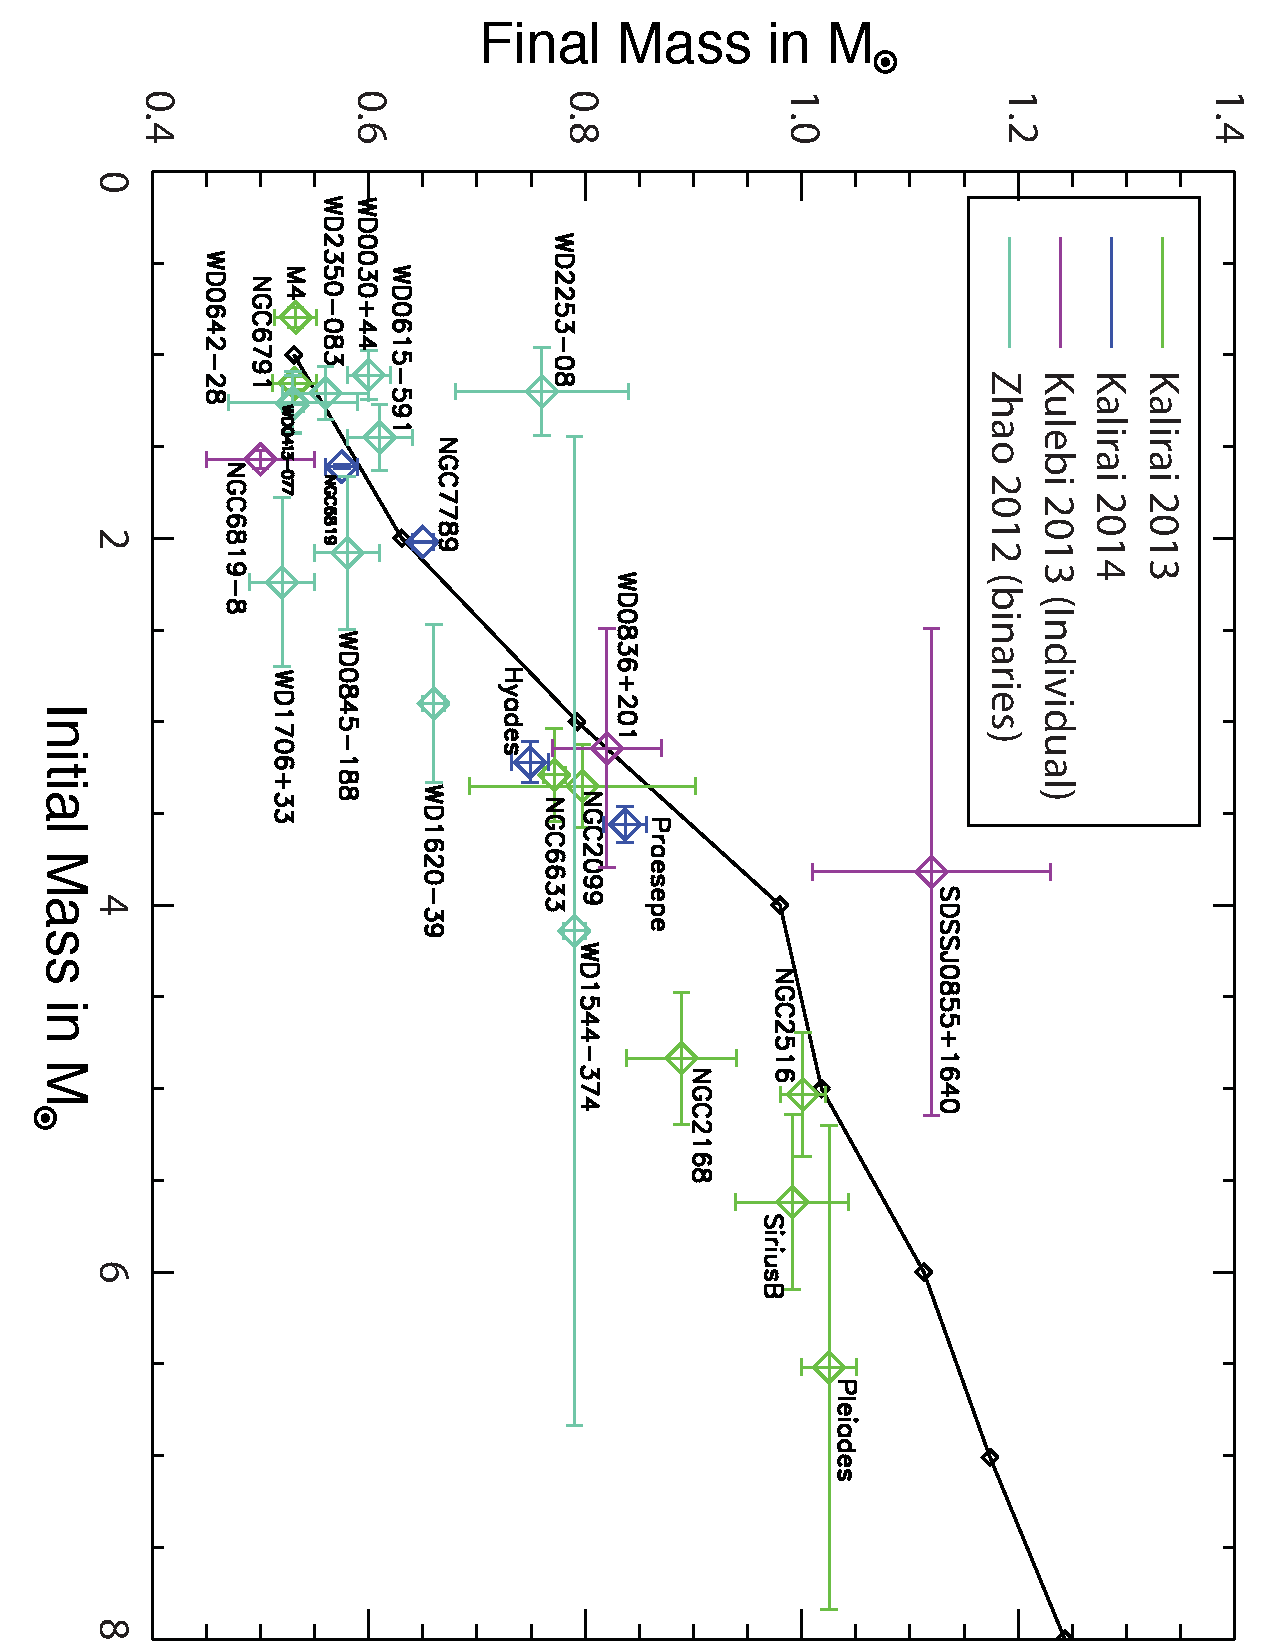
\includegraphics[width=0.35\textwidth, angle=90]{if_mod2.pdf}
\caption{ Initial final mass relation from observations and MESA calculations. The \citealt{kalirai2013a} and \citealt{kalirai2013b} points are averaged over the total observed white dwarfs in each respective cluster, while the \citealt{kulebi2013} and \citealt{zhao2012} points are taken from individual observations.}
\label{fig:ifrelation}
\end{figure} 

\begin{figure}
\centering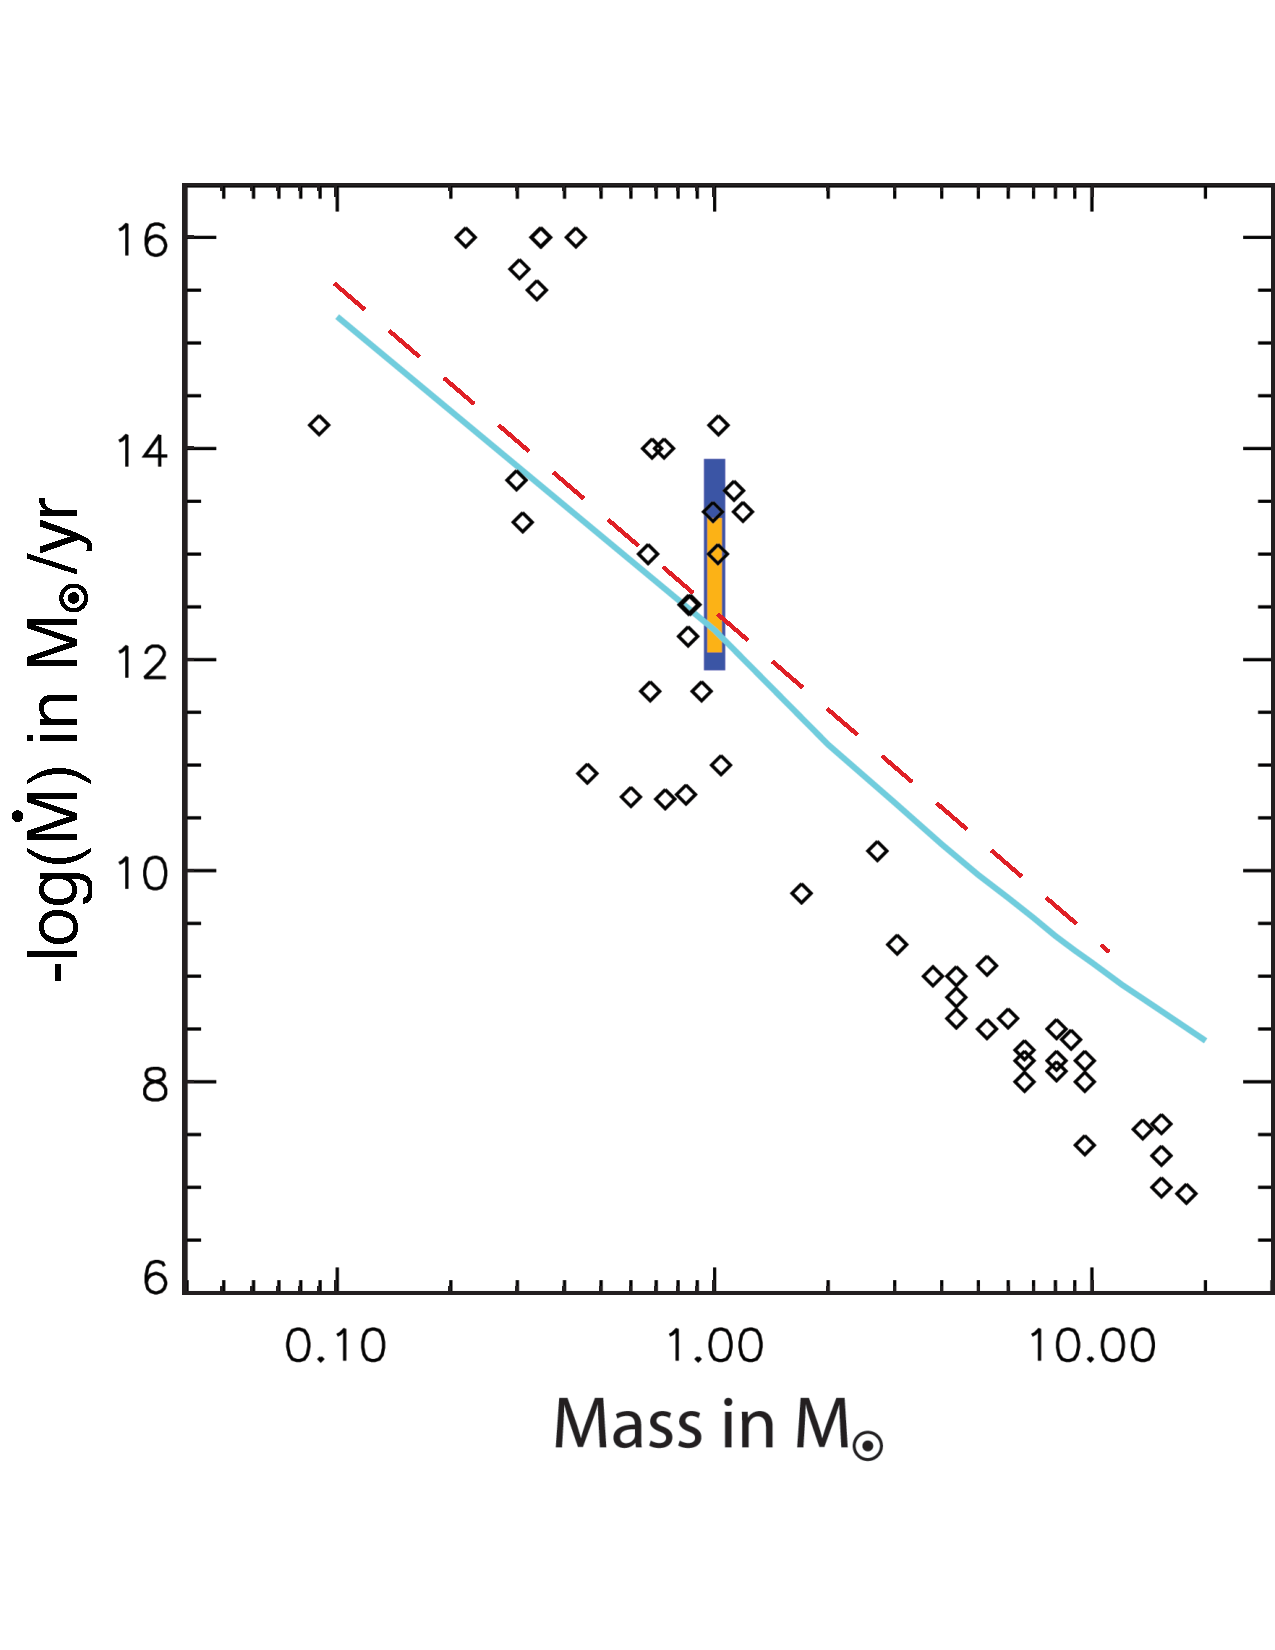
\includegraphics[width=0.46\textwidth]{mdotms_withAnalytic_mod3.pdf}
\caption{Mass loss rate estimates along the main sequence as a function of initial stellar mass.  Observational estimates are plotted as black diamonds \citep{cranmer2011,dejager1988,searle2008,waters1987,debes2006,badalyan1992,morin2008}.  The blue rectangle denotes the estimated variations in the solar mass loss rate \citep{wood2005}, and the yellow rectangle shows the observed variations in the mass loss rate of the Sun as a function of its X-ray activity \citep{cohen2011}.  The blue line shows the main sequence mass loss rate prescription used by MESA and the often derived analytical prescription is shown with the dashed red line. }
\label{fig:msmassloss}
\end{figure} 


\subsubsection{Wind Velocities}


\tikzmark{mainBodyStart2790}Shortening\tikzmark{mainBodyEnd2790} \tikzmark{mainBodyStart2791}here\tikzmark{mainBodyEnd2791} \tikzmark{mainBodyStart2792}as\tikzmark{mainBodyEnd2792} \tikzmark{mainBodyStart2793}well.\tikzmark{mainBodyEnd2793}

\subsection{Average Mass Loss and Wind Velocities as Model Inputs} \label{section:averages}

\tikzmark{mainBodyStart2794}To\tikzmark{mainBodyEnd2794} \tikzmark{mainBodyStart2795}finalize\tikzmark{mainBodyEnd2795} \tikzmark{mainBodyStart2796}our\tikzmark{mainBodyEnd2796} \tikzmark{mainBodyStart2797}mass\tikzmark{mainBodyEnd2797} \tikzmark{mainBodyStart2798}and\tikzmark{mainBodyEnd2798} \tikzmark{mainBodyStart2799}energy\tikzmark{mainBodyEnd2799} \tikzmark{mainBodyStart2800}injection\tikzmark{mainBodyEnd2800} \tikzmark{mainBodyStart2801}prescriptions\tikzmark{mainBodyEnd2801} \tikzmark{mainBodyStart2802}it\tikzmark{mainBodyEnd2802} \tikzmark{mainBodyStart2803}is\tikzmark{mainBodyEnd2803} \tikzmark{mainBodyStart2804}necessary\tikzmark{mainBodyEnd2804} \tikzmark{mainBodyStart2805}to\tikzmark{mainBodyEnd2805} \tikzmark{mainBodyStart2806}derive\tikzmark{mainBodyEnd2806} \tikzmark{mainBodyStart2807}an\tikzmark{mainBodyEnd2807} \tikzmark{mainBodyStart2808}averaged\tikzmark{mainBodyEnd2808} \tikzmark{mainBodyStart2809}mass\tikzmark{mainBodyEnd2809} \tikzmark{mainBodyStart2810}loss\tikzmark{mainBodyEnd2810} \tikzmark{mainBodyStart2811}rate\tikzmark{mainBodyEnd2811} \tikzmark{mainBodyStart2812}and\tikzmark{mainBodyEnd2812} \tikzmark{mainBodyStart2813}wind\tikzmark{mainBodyEnd2813} \tikzmark{mainBodyStart2814}velocity\tikzmark{mainBodyEnd2814} \tikzmark{mainBodyStart2815}during\tikzmark{mainBodyEnd2815} \tikzmark{mainBodyStart2816}each\tikzmark{mainBodyEnd2816} \tikzmark{mainBodyStart2817}phase\tikzmark{mainBodyEnd2817} \tikzmark{mainBodyStart2818}of\tikzmark{mainBodyEnd2818} \tikzmark{mainBodyStart2819}cluster\tikzmark{mainBodyEnd2819} \tikzmark{mainBodyStart2820}evolution\tikzmark{mainBodyEnd2820} \tikzmark{mainBodyStart2821}which\tikzmark{mainBodyEnd2821} \tikzmark{mainBodyStart2822}includes\tikzmark{mainBodyEnd2822} \tikzmark{mainBodyStart2823}contributions\tikzmark{mainBodyEnd2823} \tikzmark{mainBodyStart2824}from\tikzmark{mainBodyEnd2824} \tikzmark{mainBodyStart2825}the\tikzmark{mainBodyEnd2825} \tikzmark{mainBodyStart2826}stars\tikzmark{mainBodyEnd2826} \tikzmark{mainBodyStart2827}that\tikzmark{mainBodyEnd2827} \tikzmark{mainBodyStart2828}significantly\tikzmark{mainBodyEnd2828} \tikzmark{mainBodyStart2829}contribute\tikzmark{mainBodyEnd2829} \tikzmark{mainBodyStart2830}to\tikzmark{mainBodyEnd2830} \tikzmark{mainBodyStart2831}the\tikzmark{mainBodyEnd2831} \tikzmark{mainBodyStart2832}mass\tikzmark{mainBodyEnd2832} \tikzmark{mainBodyStart2833}and\tikzmark{mainBodyEnd2833} \tikzmark{mainBodyStart2834}kinetic\tikzmark{mainBodyEnd2834} \tikzmark{mainBodyStart2835}energy\tikzmark{mainBodyEnd2835} \tikzmark{mainBodyStart2836}injection\tikzmark{mainBodyEnd2836} \tikzmark{mainBodyStart2837}into\tikzmark{mainBodyEnd2837} \tikzmark{mainBodyStart2838}the\tikzmark{mainBodyEnd2838} \tikzmark{mainBodyStart2839}cluster.\tikzmark{mainBodyEnd2839}
\tikzmark{mainBodyStart2840}The\tikzmark{mainBodyEnd2840} \tikzmark{mainBodyStart2841}averaged\tikzmark{mainBodyEnd2841} \tikzmark{mainBodyStart2842}prescription\tikzmark{mainBodyEnd2842} \tikzmark{mainBodyStart2843}we\tikzmark{mainBodyEnd2843} \tikzmark{mainBodyStart2844}present\tikzmark{mainBodyEnd2844} \tikzmark{mainBodyStart2845}here\tikzmark{mainBodyEnd2845} \tikzmark{mainBodyStart2846}has\tikzmark{mainBodyEnd2846} \tikzmark{mainBodyStart2847}the\tikzmark{mainBodyEnd2847} \tikzmark{mainBodyStart2848}added\tikzmark{mainBodyEnd2848} \tikzmark{mainBodyStart2849}benefit\tikzmark{mainBodyEnd2849} \tikzmark{mainBodyStart2850}of\tikzmark{mainBodyEnd2850} \tikzmark{mainBodyStart2851}minimizing\tikzmark{mainBodyEnd2851} \tikzmark{mainBodyStart2852}the\tikzmark{mainBodyEnd2852} \tikzmark{mainBodyStart2853}effects\tikzmark{mainBodyEnd2853} \tikzmark{mainBodyStart2854}of\tikzmark{mainBodyEnd2854} \tikzmark{mainBodyStart2855}the\tikzmark{mainBodyEnd2855} \tikzmark{mainBodyStart2856}poorly\tikzmark{mainBodyEnd2856} \tikzmark{mainBodyStart2857}constrained,\tikzmark{mainBodyEnd2857} \tikzmark{mainBodyStart2858}rapidly\tikzmark{mainBodyEnd2858} \tikzmark{mainBodyStart2859}varying,\tikzmark{mainBodyEnd2859} \tikzmark{mainBodyStart2860}final\tikzmark{mainBodyEnd2860} \tikzmark{mainBodyStart2861}stages\tikzmark{mainBodyEnd2861} \tikzmark{mainBodyStart2862}of\tikzmark{mainBodyEnd2862} \tikzmark{mainBodyStart2863}a\tikzmark{mainBodyEnd2863} \tikzmark{mainBodyStart2864}star's\tikzmark{mainBodyEnd2864} \tikzmark{mainBodyStart2865}life\tikzmark{mainBodyEnd2865} \citep{pooley2006}


\tikzmark{mainBodyStart2866}Note:\tikzmark{mainBodyEnd2866} \tikzmark{mainBodyStart2867}more\tikzmark{mainBodyEnd2867} \tikzmark{mainBodyStart2868}shortening\tikzmark{mainBodyEnd2868} \tikzmark{mainBodyStart2869}is\tikzmark{mainBodyEnd2869} \tikzmark{mainBodyStart2870}happening\tikzmark{mainBodyEnd2870} \tikzmark{mainBodyStart2871}here\tikzmark{mainBodyEnd2871} \tikzmark{mainBodyStart2872}too.\tikzmark{mainBodyEnd2872}

\section{Applications to Various Star Clusters} \label{section:applications}

\tikzmark{mainBodyStart2873}We\tikzmark{mainBodyEnd2873} \tikzmark{mainBodyStart2874}have\tikzmark{mainBodyEnd2874} \tikzmark{mainBodyStart2875}thus\tikzmark{mainBodyEnd2875} \tikzmark{mainBodyStart2876}far\tikzmark{mainBodyEnd2876} \tikzmark{mainBodyStart2877}kept\tikzmark{mainBodyEnd2877} \tikzmark{mainBodyStart2878}our\tikzmark{mainBodyEnd2878} \tikzmark{mainBodyStart2879}discussion\tikzmark{mainBodyEnd2879} \tikzmark{mainBodyStart2880}of\tikzmark{mainBodyEnd2880} \tikzmark{mainBodyStart2881}stellar\tikzmark{mainBodyEnd2881} \tikzmark{mainBodyStart2882}wind\tikzmark{mainBodyEnd2882} \tikzmark{mainBodyStart2883}retention\tikzmark{mainBodyEnd2883} \tikzmark{mainBodyStart2884}in\tikzmark{mainBodyEnd2884} \tikzmark{mainBodyStart2885}star\tikzmark{mainBodyEnd2885} \tikzmark{mainBodyStart2886}clusters\tikzmark{mainBodyEnd2886} \tikzmark{mainBodyStart2887}generalized\tikzmark{mainBodyEnd2887} \tikzmark{mainBodyStart2888}to\tikzmark{mainBodyEnd2888} \tikzmark{mainBodyStart2889}star\tikzmark{mainBodyEnd2889} \tikzmark{mainBodyStart2890}clusters\tikzmark{mainBodyEnd2890} \tikzmark{mainBodyStart2891}with\tikzmark{mainBodyEnd2891} \tikzmark{mainBodyStart2892}different\tikzmark{mainBodyEnd2892} \tikzmark{mainBodyStart2893}combinations\tikzmark{mainBodyEnd2893} \tikzmark{mainBodyStart2894}of\tikzmark{mainBodyEnd2894} \tikzmark{mainBodyStart2895}ages,\tikzmark{mainBodyEnd2895} \tikzmark{mainBodyStart2896}masses\tikzmark{mainBodyEnd2896} \tikzmark{mainBodyStart2897}and\tikzmark{mainBodyEnd2897} \tikzmark{mainBodyStart2898}velocity\tikzmark{mainBodyEnd2898} \tikzmark{mainBodyStart2899}dispersions.\tikzmark{mainBodyEnd2899}  \tikzmark{mainBodyStart2900}In\tikzmark{mainBodyEnd2900} \tikzmark{mainBodyStart2901}what\tikzmark{mainBodyEnd2901} \tikzmark{mainBodyStart2902}follows\tikzmark{mainBodyEnd2902} \tikzmark{mainBodyStart2903}we\tikzmark{mainBodyEnd2903} \tikzmark{mainBodyStart2904}discuss\tikzmark{mainBodyEnd2904} \tikzmark{mainBodyStart2905}the\tikzmark{mainBodyEnd2905} \tikzmark{mainBodyStart2906}implications\tikzmark{mainBodyEnd2906} \tikzmark{mainBodyStart2907}of\tikzmark{mainBodyEnd2907} \tikzmark{mainBodyStart2908}gas\tikzmark{mainBodyEnd2908} \tikzmark{mainBodyStart2909}retention\tikzmark{mainBodyEnd2909} \tikzmark{mainBodyStart2910}on\tikzmark{mainBodyEnd2910} \tikzmark{mainBodyStart2911}three\tikzmark{mainBodyEnd2911} \tikzmark{mainBodyStart2912}specific\tikzmark{mainBodyEnd2912} \tikzmark{mainBodyStart2913}groups\tikzmark{mainBodyEnd2913} \tikzmark{mainBodyStart2914}of\tikzmark{mainBodyEnd2914} \tikzmark{mainBodyStart2915}star\tikzmark{mainBodyEnd2915} \tikzmark{mainBodyStart2916}clusters\tikzmark{mainBodyEnd2916} \tikzmark{mainBodyStart2917}-\tikzmark{mainBodyEnd2917} \tikzmark{mainBodyStart2918}Young\tikzmark{mainBodyEnd2918} \tikzmark{mainBodyStart2919}Massive\tikzmark{mainBodyEnd2919} \tikzmark{mainBodyStart2920}Clusters,\tikzmark{mainBodyEnd2920} \tikzmark{mainBodyStart2921}Intermediate\tikzmark{mainBodyEnd2921} \tikzmark{mainBodyStart2922}Age\tikzmark{mainBodyEnd2922} \tikzmark{mainBodyStart2923}Clusters,\tikzmark{mainBodyEnd2923} \tikzmark{mainBodyStart2924}and\tikzmark{mainBodyEnd2924} \tikzmark{mainBodyStart2925}Globular\tikzmark{mainBodyEnd2925} \tikzmark{mainBodyStart2926}Clusters\tikzmark{mainBodyEnd2926} \tikzmark{mainBodyStart2927}-\tikzmark{mainBodyEnd2927} \tikzmark{mainBodyStart2928}and\tikzmark{mainBodyEnd2928} \tikzmark{mainBodyStart2929}provide\tikzmark{mainBodyEnd2929} \tikzmark{mainBodyStart2930}limits\tikzmark{mainBodyEnd2930} \tikzmark{mainBodyStart2931}on\tikzmark{mainBodyEnd2931} \tikzmark{mainBodyStart2932}how\tikzmark{mainBodyEnd2932} \tikzmark{mainBodyStart2933}stellar\tikzmark{mainBodyEnd2933} \tikzmark{mainBodyStart2934}wind\tikzmark{mainBodyEnd2934} \tikzmark{mainBodyStart2935}retention\tikzmark{mainBodyEnd2935} \tikzmark{mainBodyStart2936}can\tikzmark{mainBodyEnd2936} \tikzmark{mainBodyStart2937}effect\tikzmark{mainBodyEnd2937} \tikzmark{mainBodyStart2938}their\tikzmark{mainBodyEnd2938} \tikzmark{mainBodyStart2939}star\tikzmark{mainBodyEnd2939} \tikzmark{mainBodyStart2940}formation\tikzmark{mainBodyEnd2940} \tikzmark{mainBodyStart2941}histories.\tikzmark{mainBodyEnd2941}


\subsection{Young Massive Clusters: Age $\lesssim$1~Gyr}

\tikzmark{mainBodyStart2942}Young,\tikzmark{mainBodyEnd2942} \tikzmark{mainBodyStart2943}massive\tikzmark{mainBodyEnd2943} \tikzmark{mainBodyStart2944}star\tikzmark{mainBodyEnd2944} \tikzmark{mainBodyStart2945}clusters\tikzmark{mainBodyEnd2945} \tikzmark{mainBodyStart2946}(YMCs)\tikzmark{mainBodyEnd2946} \tikzmark{mainBodyStart2947}are\tikzmark{mainBodyEnd2947} \tikzmark{mainBodyStart2948}ubiquitous\tikzmark{mainBodyEnd2948} \tikzmark{mainBodyStart2949}in\tikzmark{mainBodyEnd2949} \tikzmark{mainBodyStart2950}the\tikzmark{mainBodyEnd2950} \tikzmark{mainBodyStart2951}nearby\tikzmark{mainBodyEnd2951} \tikzmark{mainBodyStart2952}Small\tikzmark{mainBodyEnd2952} \tikzmark{mainBodyStart2953}and\tikzmark{mainBodyEnd2953} \tikzmark{mainBodyStart2954}Large\tikzmark{mainBodyEnd2954} \tikzmark{mainBodyStart2955}Magellanic\tikzmark{mainBodyEnd2955} \tikzmark{mainBodyStart2956}Clouds\tikzmark{mainBodyEnd2956} \citep{goud2014} \tikzmark{mainBodyStart2957}and\tikzmark{mainBodyEnd2957} \tikzmark{mainBodyStart2958}are\tikzmark{mainBodyEnd2958} \tikzmark{mainBodyStart2959}also\tikzmark{mainBodyEnd2959} \tikzmark{mainBodyStart2960}found\tikzmark{mainBodyEnd2960} \tikzmark{mainBodyStart2961}in\tikzmark{mainBodyEnd2961} \tikzmark{mainBodyStart2962}recent\tikzmark{mainBodyEnd2962} \tikzmark{mainBodyStart2963}(\tikzmark{mainBodyEnd2963}\tikzmark{mainInlineStart2964}$\lesssim$\tikzmark{mainInlineEnd2964} \tikzmark{mainBodyStart2965}mergers\tikzmark{mainBodyEnd2965} \tikzmark{mainBodyStart2966}like\tikzmark{mainBodyEnd2966} \tikzmark{mainBodyStart2967}the\tikzmark{mainBodyEnd2967} \tikzmark{mainBodyStart2968}Antennae\tikzmark{mainBodyEnd2968} \tikzmark{mainBodyStart2969}galaxies\tikzmark{mainBodyEnd2969} \citep{whitmore2007}  \tikzmark{mainBodyStart2970}As\tikzmark{mainBodyEnd2970} \tikzmark{mainBodyStart2971}one\tikzmark{mainBodyEnd2971} \tikzmark{mainBodyStart2972}of\tikzmark{mainBodyEnd2972} \tikzmark{mainBodyStart2973}the\tikzmark{mainBodyEnd2973} \tikzmark{mainBodyStart2974}canditates\tikzmark{mainBodyEnd2974} \tikzmark{mainBodyStart2975}for\tikzmark{mainBodyEnd2975} \tikzmark{mainBodyStart2976}proto-Globular\tikzmark{mainBodyEnd2976} \tikzmark{mainBodyStart2977}Clusters,\tikzmark{mainBodyEnd2977} \tikzmark{mainBodyStart2978}the\tikzmark{mainBodyEnd2978} \tikzmark{mainBodyStart2979}gas\tikzmark{mainBodyEnd2979} \tikzmark{mainBodyStart2980}content\tikzmark{mainBodyEnd2980} \tikzmark{mainBodyStart2981}and\tikzmark{mainBodyEnd2981} \tikzmark{mainBodyStart2982}star\tikzmark{mainBodyEnd2982} \tikzmark{mainBodyStart2983}formation\tikzmark{mainBodyEnd2983} \tikzmark{mainBodyStart2984}histories\tikzmark{mainBodyEnd2984} \tikzmark{mainBodyStart2985}of\tikzmark{mainBodyEnd2985} \tikzmark{mainBodyStart2986}these\tikzmark{mainBodyEnd2986} \tikzmark{mainBodyStart2987}objects\tikzmark{mainBodyEnd2987} \tikzmark{mainBodyStart2988}are\tikzmark{mainBodyEnd2988} \tikzmark{mainBodyStart2989}a\tikzmark{mainBodyEnd2989} \tikzmark{mainBodyStart2990}subject\tikzmark{mainBodyEnd2990} \tikzmark{mainBodyStart2991}of\tikzmark{mainBodyEnd2991} \tikzmark{mainBodyStart2992}much\tikzmark{mainBodyEnd2992} \tikzmark{mainBodyStart2993}interest\tikzmark{mainBodyEnd2993} \citep[e.g.][]{zwart2010}

\subsubsection{Current Gas Content} \label{section:YMCcurrent}

 \tikzmark{mainBodyStart2994}During\tikzmark{mainBodyEnd2994} \tikzmark{mainBodyStart2995}the\tikzmark{mainBodyEnd2995} \tikzmark{mainBodyStart2996}time\tikzmark{mainBodyEnd2996} \tikzmark{mainBodyStart2997}span\tikzmark{mainBodyEnd2997} \tikzmark{mainBodyStart2998}of\tikzmark{mainBodyEnd2998} \tikzmark{mainBodyStart2999}the\tikzmark{mainBodyEnd2999} \tikzmark{mainBodyStart3000}typical\tikzmark{mainBodyEnd3000} \tikzmark{mainBodyStart3001}ages\tikzmark{mainBodyEnd3001} \tikzmark{mainBodyStart3002}of\tikzmark{mainBodyEnd3002} \tikzmark{mainBodyStart3003}YMCs\tikzmark{mainBodyEnd3003} \tikzmark{mainBodyStart3004}(10s-100s~Myrs)\tikzmark{mainBodyEnd3004} \tikzmark{mainBodyStart3005}Figures\tikzmark{mainBodyEnd3005} \ref{fig:fig4} \tikzmark{mainBodyStart3006}-\tikzmark{mainBodyEnd3006} \ref{fig:memcontour} \tikzmark{mainBodyStart3007}show\tikzmark{mainBodyEnd3007} \tikzmark{mainBodyStart3008}little\tikzmark{mainBodyEnd3008} \tikzmark{mainBodyStart3009}mass\tikzmark{mainBodyEnd3009} \tikzmark{mainBodyStart3010}retention\tikzmark{mainBodyEnd3010} \tikzmark{mainBodyStart3011}and\tikzmark{mainBodyEnd3011} \tikzmark{mainBodyStart3012}star\tikzmark{mainBodyEnd3012} \tikzmark{mainBodyStart3013}formation\tikzmark{mainBodyEnd3013} \tikzmark{mainBodyStart3014}in\tikzmark{mainBodyEnd3014} \tikzmark{mainBodyStart3015}all\tikzmark{mainBodyEnd3015} \tikzmark{mainBodyStart3016}but\tikzmark{mainBodyEnd3016} \tikzmark{mainBodyStart3017}the\tikzmark{mainBodyEnd3017} \tikzmark{mainBodyStart3018}most\tikzmark{mainBodyEnd3018} \tikzmark{mainBodyStart3019}compact\tikzmark{mainBodyEnd3019} \tikzmark{mainBodyStart3020}stellar\tikzmark{mainBodyEnd3020} \tikzmark{mainBodyStart3021}clusters.\tikzmark{mainBodyEnd3021}
 \tikzmark{mainBodyStart3022}This\tikzmark{mainBodyEnd3022} \tikzmark{mainBodyStart3023}results\tikzmark{mainBodyEnd3023} \tikzmark{mainBodyStart3024}from\tikzmark{mainBodyEnd3024} \tikzmark{mainBodyStart3025}the\tikzmark{mainBodyEnd3025} \tikzmark{mainBodyStart3026}fast\tikzmark{mainBodyEnd3026} \tikzmark{mainBodyStart3027}winds\tikzmark{mainBodyEnd3027} \tikzmark{mainBodyStart3028}from\tikzmark{mainBodyEnd3028} \tikzmark{mainBodyStart3029}main\tikzmark{mainBodyEnd3029} \tikzmark{mainBodyStart3030}sequence\tikzmark{mainBodyEnd3030} \tikzmark{mainBodyStart3031}O\tikzmark{mainBodyEnd3031} \tikzmark{mainBodyStart3032}and\tikzmark{mainBodyEnd3032} \tikzmark{mainBodyStart3033}B\tikzmark{mainBodyEnd3033} \tikzmark{mainBodyStart3034}stars\tikzmark{mainBodyEnd3034} \tikzmark{mainBodyStart3035}as\tikzmark{mainBodyEnd3035} \tikzmark{mainBodyStart3036}shown\tikzmark{mainBodyEnd3036} \tikzmark{mainBodyStart3037}in\tikzmark{mainBodyEnd3037} \tikzmark{mainBodyStart3038}Figure\tikzmark{mainBodyEnd3038} \ref{fig:fig1} \tikzmark{mainBodyStart3039}for\tikzmark{mainBodyEnd3039} \tikzmark{mainBodyStart3040}ages\tikzmark{mainBodyEnd3040} \tikzmark{mainInlineStart3041}$\lesssim 20$\tikzmark{mainInlineEnd3041} \tikzmark{mainBodyStart3042}and\tikzmark{mainBodyEnd3042} \tikzmark{mainBodyStart3043}the\tikzmark{mainBodyEnd3043} \tikzmark{mainBodyStart3044}lack\tikzmark{mainBodyEnd3044} \tikzmark{mainBodyStart3045}of\tikzmark{mainBodyEnd3045} \tikzmark{mainBodyStart3046}sufficient\tikzmark{mainBodyEnd3046} \tikzmark{mainBodyStart3047}gas\tikzmark{mainBodyEnd3047} \tikzmark{mainBodyStart3048}accumulation\tikzmark{mainBodyEnd3048} \tikzmark{mainBodyStart3049}time\tikzmark{mainBodyEnd3049} \tikzmark{mainBodyStart3050}to\tikzmark{mainBodyEnd3050} \tikzmark{mainBodyStart3051}initiate\tikzmark{mainBodyEnd3051} \tikzmark{mainBodyStart3052}runaway\tikzmark{mainBodyEnd3052} \tikzmark{mainBodyStart3053}cooling\tikzmark{mainBodyEnd3053} \tikzmark{mainBodyStart3054}and\tikzmark{mainBodyEnd3054} \tikzmark{mainBodyStart3055}collapse\tikzmark{mainBodyEnd3055} \tikzmark{mainBodyStart3056}for\tikzmark{mainBodyEnd3056} \tikzmark{mainBodyStart3057}clusters\tikzmark{mainBodyEnd3057} \tikzmark{mainBodyStart3058}with\tikzmark{mainBodyEnd3058} \tikzmark{mainInlineStart3059}$20 \lesssim{\rm age/Myrs} \lesssim 500$\tikzmark{mainInlineEnd3059}
 \tikzmark{mainBodyStart3060}For\tikzmark{mainBodyEnd3060} \tikzmark{mainBodyStart3061}clusters\tikzmark{mainBodyEnd3061} \tikzmark{mainBodyStart3062}with\tikzmark{mainBodyEnd3062} \tikzmark{mainBodyStart3063}large\tikzmark{mainBodyEnd3063} \tikzmark{mainBodyStart3064}velocity\tikzmark{mainBodyEnd3064} \tikzmark{mainBodyStart3065}dispersions,\tikzmark{mainBodyEnd3065} \tikzmark{mainInlineStart3066}$\sigma_v \gtrsim 35 \, {\rm km s^{-1}}$\tikzmark{mainInlineEnd3066} \tikzmark{mainBodyStart3067}while\tikzmark{mainBodyEnd3067} \tikzmark{mainBodyStart3068}some\tikzmark{mainBodyEnd3068} \tikzmark{mainBodyStart3069}gas\tikzmark{mainBodyEnd3069} \tikzmark{mainBodyStart3070}mass\tikzmark{mainBodyEnd3070} \tikzmark{mainBodyStart3071}is\tikzmark{mainBodyEnd3071} \tikzmark{mainBodyStart3072}retained\tikzmark{mainBodyEnd3072} \tikzmark{mainBodyStart3073}and\tikzmark{mainBodyEnd3073} \tikzmark{mainBodyStart3074}star\tikzmark{mainBodyEnd3074} \tikzmark{mainBodyStart3075}formation\tikzmark{mainBodyEnd3075} \tikzmark{mainBodyStart3076}is\tikzmark{mainBodyEnd3076} \tikzmark{mainBodyStart3077}triggered,\tikzmark{mainBodyEnd3077} \tikzmark{mainBodyStart3078}less\tikzmark{mainBodyEnd3078} \tikzmark{mainBodyStart3079}than\tikzmark{mainBodyEnd3079} \tikzmark{mainInlineStart3080}$\approx 2$\tikzmark{mainInlineEnd3080} \tikzmark{mainBodyStart3081}of\tikzmark{mainBodyEnd3081} \tikzmark{mainBodyStart3082}the\tikzmark{mainBodyEnd3082} \tikzmark{mainBodyStart3083}original\tikzmark{mainBodyEnd3083} \tikzmark{mainBodyStart3084}cluster's\tikzmark{mainBodyEnd3084} \tikzmark{mainBodyStart3085}mass\tikzmark{mainBodyEnd3085} \tikzmark{mainBodyStart3086}is\tikzmark{mainBodyEnd3086} \tikzmark{mainBodyStart3087}available\tikzmark{mainBodyEnd3087} \tikzmark{mainBodyStart3088}for\tikzmark{mainBodyEnd3088} \tikzmark{mainBodyStart3089}star\tikzmark{mainBodyEnd3089} \tikzmark{mainBodyStart3090}formation.\tikzmark{mainBodyEnd3090}

 \tikzmark{mainBodyStart3091}In\tikzmark{mainBodyEnd3091} \tikzmark{mainBodyStart3092}such\tikzmark{mainBodyEnd3092} \tikzmark{mainBodyStart3093}clusters\tikzmark{mainBodyEnd3093} \tikzmark{mainBodyStart3094}we\tikzmark{mainBodyEnd3094} \tikzmark{mainBodyStart3095}expect\tikzmark{mainBodyEnd3095} \tikzmark{mainBodyStart3096}several\tikzmark{mainBodyEnd3096} \tikzmark{mainBodyStart3097}additional\tikzmark{mainBodyEnd3097} \tikzmark{mainBodyStart3098}mechanisms\tikzmark{mainBodyEnd3098} \tikzmark{mainBodyStart3099}to\tikzmark{mainBodyEnd3099} \tikzmark{mainBodyStart3100}add\tikzmark{mainBodyEnd3100} \tikzmark{mainBodyStart3101}significantly\tikzmark{mainBodyEnd3101} \tikzmark{mainBodyStart3102}to\tikzmark{mainBodyEnd3102} \tikzmark{mainBodyStart3103}the\tikzmark{mainBodyEnd3103} \tikzmark{mainBodyStart3104}energy\tikzmark{mainBodyEnd3104} \tikzmark{mainBodyStart3105}injection\tikzmark{mainBodyEnd3105} \tikzmark{mainBodyStart3106}rate\tikzmark{mainBodyEnd3106} \tikzmark{mainBodyStart3107}in\tikzmark{mainBodyEnd3107} \tikzmark{mainBodyStart3108}the\tikzmark{mainBodyEnd3108} \tikzmark{mainBodyStart3109}intercluster\tikzmark{mainBodyEnd3109} \tikzmark{mainBodyStart3110}gas.\tikzmark{mainBodyEnd3110}
 \tikzmark{mainBodyStart3111}As\tikzmark{mainBodyEnd3111} \tikzmark{mainBodyStart3112}shown\tikzmark{mainBodyEnd3112} \tikzmark{mainBodyStart3113}in\tikzmark{mainBodyEnd3113} \cite{calura2015} \tikzmark{mainBodyStart3114}SNe\tikzmark{mainBodyEnd3114} \tikzmark{mainBodyStart3115}can\tikzmark{mainBodyEnd3115} \tikzmark{mainBodyStart3116}be\tikzmark{mainBodyEnd3116} \tikzmark{mainBodyStart3117}an\tikzmark{mainBodyEnd3117} \tikzmark{mainBodyStart3118}effective\tikzmark{mainBodyEnd3118} \tikzmark{mainBodyStart3119}avenue\tikzmark{mainBodyEnd3119} \tikzmark{mainBodyStart3120}to\tikzmark{mainBodyEnd3120} \tikzmark{mainBodyStart3121}assist\tikzmark{mainBodyEnd3121} \tikzmark{mainBodyStart3122}in\tikzmark{mainBodyEnd3122} \tikzmark{mainBodyStart3123}the\tikzmark{mainBodyEnd3123} \tikzmark{mainBodyStart3124}removal\tikzmark{mainBodyEnd3124} \tikzmark{mainBodyStart3125}of\tikzmark{mainBodyEnd3125} \tikzmark{mainBodyStart3126}gas\tikzmark{mainBodyEnd3126} \tikzmark{mainBodyStart3127}from\tikzmark{mainBodyEnd3127} \tikzmark{mainBodyStart3128}stellar\tikzmark{mainBodyEnd3128} \tikzmark{mainBodyStart3129}clusters,\tikzmark{mainBodyEnd3129} \tikzmark{mainBodyStart3130}though\tikzmark{mainBodyEnd3130} \tikzmark{mainBodyStart3131}in\tikzmark{mainBodyEnd3131} \tikzmark{mainBodyStart3132}some\tikzmark{mainBodyEnd3132} \tikzmark{mainBodyStart3133}systems\tikzmark{mainBodyEnd3133} \tikzmark{mainBodyStart3134}SNe\tikzmark{mainBodyEnd3134} \tikzmark{mainBodyStart3135}alone\tikzmark{mainBodyEnd3135} \tikzmark{mainBodyStart3136}may\tikzmark{mainBodyEnd3136} \tikzmark{mainBodyStart3137}not\tikzmark{mainBodyEnd3137} \tikzmark{mainBodyStart3138}be\tikzmark{mainBodyEnd3138} \tikzmark{mainBodyStart3139}able\tikzmark{mainBodyEnd3139} \tikzmark{mainBodyStart3140}to\tikzmark{mainBodyEnd3140} \tikzmark{mainBodyStart3141}fully\tikzmark{mainBodyEnd3141} \tikzmark{mainBodyStart3142}remove\tikzmark{mainBodyEnd3142} \tikzmark{mainBodyStart3143}gas\tikzmark{mainBodyEnd3143} \tikzmark{mainBodyStart3144}from\tikzmark{mainBodyEnd3144} \tikzmark{mainBodyStart3145}young\tikzmark{mainBodyEnd3145} \tikzmark{mainBodyStart3146}clusters\tikzmark{mainBodyEnd3146} \citep{krause2013}
 \tikzmark{mainBodyStart3147}In\tikzmark{mainBodyEnd3147} \tikzmark{mainBodyStart3148}addition,\tikzmark{mainBodyEnd3148} \tikzmark{mainBodyStart3149}accretion\tikzmark{mainBodyEnd3149} \tikzmark{mainBodyStart3150}onto\tikzmark{mainBodyEnd3150} \tikzmark{mainBodyStart3151}compact\tikzmark{mainBodyEnd3151} \tikzmark{mainBodyStart3152}objects\tikzmark{mainBodyEnd3152} \tikzmark{mainBodyStart3153}may\tikzmark{mainBodyEnd3153} \tikzmark{mainBodyStart3154}be\tikzmark{mainBodyEnd3154} \tikzmark{mainBodyStart3155}able\tikzmark{mainBodyEnd3155} \tikzmark{mainBodyStart3156}to\tikzmark{mainBodyEnd3156} \tikzmark{mainBodyStart3157}clear\tikzmark{mainBodyEnd3157} \tikzmark{mainBodyStart3158}gas\tikzmark{mainBodyEnd3158} \tikzmark{mainBodyStart3159}within\tikzmark{mainBodyEnd3159} \tikzmark{mainBodyStart3160}YMCs\tikzmark{mainBodyEnd3160} \tikzmark{mainBodyStart3161}on\tikzmark{mainBodyEnd3161} \tikzmark{mainBodyStart3162}time\tikzmark{mainBodyEnd3162} \tikzmark{mainBodyStart3163}scales\tikzmark{mainBodyEnd3163} \tikzmark{mainBodyStart3164}as\tikzmark{mainBodyEnd3164} \tikzmark{mainBodyStart3165}small\tikzmark{mainBodyEnd3165} \tikzmark{mainBodyStart3166}as\tikzmark{mainBodyEnd3166} \tikzmark{mainBodyStart3167}10~Myrs\tikzmark{mainBodyEnd3167} \citep{leigh2013a}
 \tikzmark{mainBodyStart3168}Finally,\tikzmark{mainBodyEnd3168} \tikzmark{mainBodyStart3169}Lyman-Werner\tikzmark{mainBodyEnd3169} \tikzmark{mainBodyStart3170}flux\tikzmark{mainBodyEnd3170} \tikzmark{mainBodyStart3171}from\tikzmark{mainBodyEnd3171} \tikzmark{mainBodyStart3172}massive\tikzmark{mainBodyEnd3172} \tikzmark{mainBodyStart3173}stars\tikzmark{mainBodyEnd3173} \tikzmark{mainBodyStart3174}further\tikzmark{mainBodyEnd3174} \tikzmark{mainBodyStart3175}inhibits\tikzmark{mainBodyEnd3175} \tikzmark{mainBodyStart3176}star\tikzmark{mainBodyEnd3176} \tikzmark{mainBodyStart3177}formation\tikzmark{mainBodyEnd3177} \tikzmark{mainBodyStart3178}by\tikzmark{mainBodyEnd3178} \tikzmark{mainBodyStart3179}dissassociating\tikzmark{mainBodyEnd3179} \tikzmark{mainBodyStart3180}molecular\tikzmark{mainBodyEnd3180} \tikzmark{mainBodyStart3181}hydrogen\tikzmark{mainBodyEnd3181} \tikzmark{mainBodyStart3182}in\tikzmark{mainBodyEnd3182} \tikzmark{mainBodyStart3183}these\tikzmark{mainBodyEnd3183} \tikzmark{mainBodyStart3184}young\tikzmark{mainBodyEnd3184} \tikzmark{mainBodyStart3185}systems\tikzmark{mainBodyEnd3185} \citep{ten1986,conroy2011b,krause2013}
 \tikzmark{mainBodyStart3186}Therefore,\tikzmark{mainBodyEnd3186} \tikzmark{mainBodyStart3187}we\tikzmark{mainBodyEnd3187} \tikzmark{mainBodyStart3188}conclude\tikzmark{mainBodyEnd3188} \tikzmark{mainBodyStart3189}that\tikzmark{mainBodyEnd3189} \tikzmark{mainBodyStart3190}our\tikzmark{mainBodyEnd3190} \tikzmark{mainBodyStart3191}estimates\tikzmark{mainBodyEnd3191} \tikzmark{mainBodyStart3192}of\tikzmark{mainBodyEnd3192} \tikzmark{mainBodyStart3193}gas\tikzmark{mainBodyEnd3193} \tikzmark{mainBodyStart3194}retention\tikzmark{mainBodyEnd3194} \tikzmark{mainBodyStart3195}on\tikzmark{mainBodyEnd3195} \tikzmark{mainBodyStart3196}the\tikzmark{mainBodyEnd3196} \tikzmark{mainBodyStart3197}order\tikzmark{mainBodyEnd3197} \tikzmark{mainBodyStart3198}of\tikzmark{mainBodyEnd3198} \tikzmark{mainBodyStart3199}a\tikzmark{mainBodyEnd3199} \tikzmark{mainBodyStart3200}few\tikzmark{mainBodyEnd3200} \tikzmark{mainBodyStart3201}percent\tikzmark{mainBodyEnd3201} \tikzmark{mainBodyStart3202}are\tikzmark{mainBodyEnd3202} \tikzmark{mainBodyStart3203}upper\tikzmark{mainBodyEnd3203} \tikzmark{mainBodyStart3204}limits\tikzmark{mainBodyEnd3204} \tikzmark{mainBodyStart3205}for\tikzmark{mainBodyEnd3205} \tikzmark{mainBodyStart3206}the\tikzmark{mainBodyEnd3206} \tikzmark{mainBodyStart3207}total\tikzmark{mainBodyEnd3207} \tikzmark{mainBodyStart3208}mass\tikzmark{mainBodyEnd3208} \tikzmark{mainBodyStart3209}retained\tikzmark{mainBodyEnd3209} \tikzmark{mainBodyStart3210}from\tikzmark{mainBodyEnd3210} \tikzmark{mainBodyStart3211}stellar\tikzmark{mainBodyEnd3211} \tikzmark{mainBodyStart3212}wind\tikzmark{mainBodyEnd3212} \tikzmark{mainBodyStart3213}ejecta\tikzmark{mainBodyEnd3213} \tikzmark{mainBodyStart3214}within\tikzmark{mainBodyEnd3214} \tikzmark{mainBodyStart3215}YMCs.\tikzmark{mainBodyEnd3215}

 \tikzmark{mainBodyStart3216}Such\tikzmark{mainBodyEnd3216} \tikzmark{mainBodyStart3217}a\tikzmark{mainBodyEnd3217} \tikzmark{mainBodyStart3218}small\tikzmark{mainBodyEnd3218} \tikzmark{mainBodyStart3219}amount\tikzmark{mainBodyEnd3219} \tikzmark{mainBodyStart3220}of\tikzmark{mainBodyEnd3220} \tikzmark{mainBodyStart3221}gas\tikzmark{mainBodyEnd3221} \tikzmark{mainBodyStart3222}retention\tikzmark{mainBodyEnd3222} \tikzmark{mainBodyStart3223}is\tikzmark{mainBodyEnd3223} \tikzmark{mainBodyStart3224}broadly\tikzmark{mainBodyEnd3224} \tikzmark{mainBodyStart3225}consistent\tikzmark{mainBodyEnd3225} \tikzmark{mainBodyStart3226}with\tikzmark{mainBodyEnd3226} \tikzmark{mainBodyStart3227}both\tikzmark{mainBodyEnd3227} \tikzmark{mainBodyStart3228}observations\tikzmark{mainBodyEnd3228} \tikzmark{mainBodyStart3229}and\tikzmark{mainBodyEnd3229} \tikzmark{mainBodyStart3230}more\tikzmark{mainBodyEnd3230} \tikzmark{mainBodyStart3231}complex\tikzmark{mainBodyEnd3231} \tikzmark{mainBodyStart3232}simulations.\tikzmark{mainBodyEnd3232}
 \tikzmark{mainBodyStart3233}Recent\tikzmark{mainBodyEnd3233} \tikzmark{mainBodyStart3234}observations\tikzmark{mainBodyEnd3234} \tikzmark{mainBodyStart3235}which\tikzmark{mainBodyEnd3235} \tikzmark{mainBodyStart3236}show\tikzmark{mainBodyEnd3236} \tikzmark{mainBodyStart3237}little\tikzmark{mainBodyEnd3237} \tikzmark{mainBodyStart3238}gas\tikzmark{mainBodyEnd3238} \tikzmark{mainBodyStart3239}in\tikzmark{mainBodyEnd3239} \tikzmark{mainBodyStart3240}all\tikzmark{mainBodyEnd3240} \tikzmark{mainBodyStart3241}but\tikzmark{mainBodyEnd3241} \tikzmark{mainBodyStart3242}the\tikzmark{mainBodyEnd3242} \tikzmark{mainBodyStart3243}most\tikzmark{mainBodyEnd3243} \tikzmark{mainBodyStart3244}compact\tikzmark{mainBodyEnd3244} \tikzmark{mainBodyStart3245}clusters\tikzmark{mainBodyEnd3245} \citep{bastian2014a,cabrera2015,krui2015,longmore2015} \tikzmark{mainBodyStart3246}though\tikzmark{mainBodyEnd3246} \tikzmark{mainBodyStart3247}observations\tikzmark{mainBodyEnd3247} \tikzmark{mainBodyStart3248}at\tikzmark{mainBodyEnd3248} \tikzmark{mainBodyStart3249}high\tikzmark{mainBodyEnd3249} \tikzmark{mainBodyStart3250}redshift\tikzmark{mainBodyEnd3250} \tikzmark{mainBodyStart3251}are\tikzmark{mainBodyEnd3251} \tikzmark{mainBodyStart3252}challenging\tikzmark{mainBodyEnd3252} \citep{longmore2015}
 \tikzmark{mainBodyStart3253}Our\tikzmark{mainBodyEnd3253} \tikzmark{mainBodyStart3254}results\tikzmark{mainBodyEnd3254} \tikzmark{mainBodyStart3255}are\tikzmark{mainBodyEnd3255} \tikzmark{mainBodyStart3256}also\tikzmark{mainBodyEnd3256} \tikzmark{mainBodyStart3257}consistent\tikzmark{mainBodyEnd3257} \tikzmark{mainBodyStart3258}with\tikzmark{mainBodyEnd3258} \tikzmark{mainBodyStart3259}analytic\tikzmark{mainBodyEnd3259} \tikzmark{mainBodyStart3260}and\tikzmark{mainBodyEnd3260} \tikzmark{mainBodyStart3261}three\tikzmark{mainBodyEnd3261} \tikzmark{mainBodyStart3262}dimensional\tikzmark{mainBodyEnd3262} \tikzmark{mainBodyStart3263}simulations\tikzmark{mainBodyEnd3263} \tikzmark{mainBodyStart3264}of\tikzmark{mainBodyEnd3264}  \tikzmark{mainBodyStart3265}which\tikzmark{mainBodyEnd3265} \tikzmark{mainBodyStart3266}find\tikzmark{mainBodyEnd3266} \tikzmark{mainBodyStart3267}that\tikzmark{mainBodyEnd3267} \tikzmark{mainBodyStart3268}the\tikzmark{mainBodyEnd3268} \tikzmark{mainBodyStart3269}majority\tikzmark{mainBodyEnd3269} \tikzmark{mainBodyStart3270}of\tikzmark{mainBodyEnd3270} \tikzmark{mainBodyStart3271}gas\tikzmark{mainBodyEnd3271} \tikzmark{mainBodyStart3272}mass\tikzmark{mainBodyEnd3272} \tikzmark{mainBodyStart3273}is\tikzmark{mainBodyEnd3273} \tikzmark{mainBodyStart3274}removed\tikzmark{mainBodyEnd3274} \tikzmark{mainBodyStart3275}by\tikzmark{mainBodyEnd3275} \tikzmark{mainInlineStart3276}$1-14$\tikzmark{mainInlineEnd3276} \citep{calura2015,krui2015}


\subsubsection{Previous and Ongoing Star Formation} \label{section:YMCongoing}

 \tikzmark{mainBodyStart3277}Our\tikzmark{mainBodyEnd3277} \tikzmark{mainBodyStart3278}results\tikzmark{mainBodyEnd3278} \tikzmark{mainBodyStart3279}of\tikzmark{mainBodyEnd3279} \tikzmark{mainBodyStart3280}little\tikzmark{mainBodyEnd3280} \tikzmark{mainBodyStart3281}to\tikzmark{mainBodyEnd3281} \tikzmark{mainBodyStart3282}no\tikzmark{mainBodyEnd3282} \tikzmark{mainBodyStart3283}star\tikzmark{mainBodyEnd3283} \tikzmark{mainBodyStart3284}formation\tikzmark{mainBodyEnd3284} \tikzmark{mainBodyStart3285}in\tikzmark{mainBodyEnd3285} \tikzmark{mainBodyStart3286}Figures\tikzmark{mainBodyEnd3286} \ref{fig:fig4} \tikzmark{mainBodyStart3287}-\tikzmark{mainBodyEnd3287} \ref{fig:memcontour} \tikzmark{mainBodyStart3288}over\tikzmark{mainBodyEnd3288} \tikzmark{mainBodyStart3289}the\tikzmark{mainBodyEnd3289} \tikzmark{mainBodyStart3290}several\tikzmark{mainBodyEnd3290} \tikzmark{mainBodyStart3291}hundreds\tikzmark{mainBodyEnd3291} \tikzmark{mainBodyStart3292}of\tikzmark{mainBodyEnd3292} \tikzmark{mainBodyStart3293}Myrs\tikzmark{mainBodyEnd3293} \tikzmark{mainBodyStart3294}timespan\tikzmark{mainBodyEnd3294} \tikzmark{mainBodyStart3295}are\tikzmark{mainBodyEnd3295} \tikzmark{mainBodyStart3296}broadly\tikzmark{mainBodyEnd3296} \tikzmark{mainBodyStart3297}consistent\tikzmark{mainBodyEnd3297} \tikzmark{mainBodyStart3298}with\tikzmark{mainBodyEnd3298} \tikzmark{mainBodyStart3299}the\tikzmark{mainBodyEnd3299} \tikzmark{mainBodyStart3300}results\tikzmark{mainBodyEnd3300} \tikzmark{mainBodyStart3301}of\tikzmark{mainBodyEnd3301} \cite{bastian2013a} \tikzmark{mainBodyStart3302}which\tikzmark{mainBodyEnd3302} \tikzmark{mainBodyStart3303}show\tikzmark{mainBodyEnd3303} \tikzmark{mainBodyStart3304}no\tikzmark{mainBodyEnd3304} \tikzmark{mainBodyStart3305}ongoing\tikzmark{mainBodyEnd3305} \tikzmark{mainBodyStart3306}star\tikzmark{mainBodyEnd3306} \tikzmark{mainBodyStart3307}formation\tikzmark{mainBodyEnd3307} \tikzmark{mainBodyStart3308}in\tikzmark{mainBodyEnd3308} \tikzmark{mainBodyStart3309}130\tikzmark{mainBodyEnd3309} \tikzmark{mainBodyStart3310}YMCs\tikzmark{mainBodyEnd3310} \tikzmark{mainBodyStart3311}with\tikzmark{mainBodyEnd3311} \tikzmark{mainBodyStart3312}masses\tikzmark{mainBodyEnd3312} \tikzmark{mainBodyStart3313}ranging\tikzmark{mainBodyEnd3313} \tikzmark{mainBodyStart3314}from\tikzmark{mainBodyEnd3314} \tikzmark{mainInlineStart3315}$10^4 < M/M_\odot < 10^8$\tikzmark{mainInlineEnd3315} \tikzmark{mainBodyStart3316}and\tikzmark{mainBodyEnd3316} \tikzmark{mainBodyStart3317}ages\tikzmark{mainBodyEnd3317} \tikzmark{mainInlineStart3318}$10 < {\rm age/Myrs} < 1000$\tikzmark{mainInlineEnd3318} \tikzmark{mainBodyStart3319}and\tikzmark{mainBodyEnd3319} \cite{mart2018} \tikzmark{mainBodyStart3320}who\tikzmark{mainBodyEnd3320} \tikzmark{mainBodyStart3321}only\tikzmark{mainBodyEnd3321} \tikzmark{mainBodyStart3322}find\tikzmark{mainBodyEnd3322} \tikzmark{mainBodyStart3323}MSPs\tikzmark{mainBodyEnd3323} \tikzmark{mainBodyStart3324}in\tikzmark{mainBodyEnd3324} \tikzmark{mainBodyStart3325}clusters\tikzmark{mainBodyEnd3325} \tikzmark{mainBodyStart3326}with\tikzmark{mainBodyEnd3326} \tikzmark{mainBodyStart3327}ages\tikzmark{mainBodyEnd3327} \tikzmark{mainInlineStart3328}$\gtrsim 2$\tikzmark{mainInlineEnd3328} \tikzmark{mainBodyStart3329}though\tikzmark{mainBodyEnd3329} \tikzmark{mainBodyStart3330}our\tikzmark{mainBodyEnd3330} \tikzmark{mainBodyStart3331}level\tikzmark{mainBodyEnd3331} \tikzmark{mainBodyStart3332}of\tikzmark{mainBodyEnd3332} \tikzmark{mainBodyStart3333}predicted\tikzmark{mainBodyEnd3333} \tikzmark{mainBodyStart3334}star\tikzmark{mainBodyEnd3334} \tikzmark{mainBodyStart3335}formation\tikzmark{mainBodyEnd3335} \tikzmark{mainBodyStart3336}may\tikzmark{mainBodyEnd3336} \tikzmark{mainBodyStart3337}be\tikzmark{mainBodyEnd3337} \tikzmark{mainBodyStart3338}too\tikzmark{mainBodyEnd3338} \tikzmark{mainBodyStart3339}low\tikzmark{mainBodyEnd3339} \tikzmark{mainBodyStart3340}to\tikzmark{mainBodyEnd3340} \tikzmark{mainBodyStart3341}be\tikzmark{mainBodyEnd3341} \tikzmark{mainBodyStart3342}detectable\tikzmark{mainBodyEnd3342} \tikzmark{mainBodyStart3343}in\tikzmark{mainBodyEnd3343} \tikzmark{mainBodyStart3344}the\tikzmark{mainBodyEnd3344} \tikzmark{mainBodyStart3345}majority\tikzmark{mainBodyEnd3345} \tikzmark{mainBodyStart3346}of\tikzmark{mainBodyEnd3346} \tikzmark{mainBodyStart3347}YMCs\tikzmark{mainBodyEnd3347} \citep{peacock2013}
  \tikzmark{mainBodyStart3348}Our\tikzmark{mainBodyEnd3348} \tikzmark{mainBodyStart3349}limit\tikzmark{mainBodyEnd3349} \tikzmark{mainBodyStart3350}of\tikzmark{mainBodyEnd3350} \tikzmark{mainInlineStart3351}$\sigma_v \gtrsim 35 \, {\rm km s^{-1}}$\tikzmark{mainInlineEnd3351} \tikzmark{mainBodyStart3352}is\tikzmark{mainBodyEnd3352} \tikzmark{mainBodyStart3353}a\tikzmark{mainBodyEnd3353} \tikzmark{mainBodyStart3354}slightly\tikzmark{mainBodyEnd3354} \tikzmark{mainBodyStart3355}higher\tikzmark{mainBodyEnd3355} \tikzmark{mainBodyStart3356}limit\tikzmark{mainBodyEnd3356} \tikzmark{mainBodyStart3357}for\tikzmark{mainBodyEnd3357} \tikzmark{mainBodyStart3358}velocity\tikzmark{mainBodyEnd3358} \tikzmark{mainBodyStart3359}dispersion\tikzmark{mainBodyEnd3359} \tikzmark{mainBodyStart3360}than\tikzmark{mainBodyEnd3360} \tikzmark{mainBodyStart3361}that\tikzmark{mainBodyEnd3361} \tikzmark{mainBodyStart3362}derived\tikzmark{mainBodyEnd3362} \tikzmark{mainBodyStart3363}observationally\tikzmark{mainBodyEnd3363} \tikzmark{mainBodyStart3364}from\tikzmark{mainBodyEnd3364} \tikzmark{mainBodyStart3365}assuming\tikzmark{mainBodyEnd3365} \tikzmark{mainBodyStart3366}eMSTO\tikzmark{mainBodyEnd3366} \tikzmark{mainBodyStart3367}features\tikzmark{mainBodyEnd3367} \tikzmark{mainBodyStart3368}in\tikzmark{mainBodyEnd3368} \tikzmark{mainBodyStart3369}IACs\tikzmark{mainBodyEnd3369} \citep{goud2014} \tikzmark{mainBodyStart3370}are\tikzmark{mainBodyEnd3370} \tikzmark{mainBodyStart3371}due\tikzmark{mainBodyEnd3371} \tikzmark{mainBodyStart3372}to\tikzmark{mainBodyEnd3372} \tikzmark{mainBodyStart3373}an\tikzmark{mainBodyEnd3373} \tikzmark{mainBodyStart3374}age\tikzmark{mainBodyEnd3374} \tikzmark{mainBodyStart3375}spread.\tikzmark{mainBodyEnd3375}  \tikzmark{mainBodyStart3376}Such\tikzmark{mainBodyEnd3376} \tikzmark{mainBodyStart3377}a\tikzmark{mainBodyEnd3377} \tikzmark{mainBodyStart3378}discrepancy\tikzmark{mainBodyEnd3378} \tikzmark{mainBodyStart3379}can\tikzmark{mainBodyEnd3379} \tikzmark{mainBodyStart3380}be\tikzmark{mainBodyEnd3380} \tikzmark{mainBodyStart3381}alleviated\tikzmark{mainBodyEnd3381} \tikzmark{mainBodyStart3382}if\tikzmark{mainBodyEnd3382} \tikzmark{mainBodyStart3383}assumed\tikzmark{mainBodyEnd3383} \tikzmark{mainBodyStart3384}evolution\tikzmark{mainBodyEnd3384} \tikzmark{mainBodyStart3385}of\tikzmark{mainBodyEnd3385} \tikzmark{mainBodyStart3386}the\tikzmark{mainBodyEnd3386} \tikzmark{mainBodyStart3387}velocity\tikzmark{mainBodyEnd3387} \tikzmark{mainBodyStart3388}dispersion\tikzmark{mainBodyEnd3388} \tikzmark{mainBodyStart3389}changes\tikzmark{mainBodyEnd3389} \tikzmark{mainBodyStart3390}more\tikzmark{mainBodyEnd3390} \tikzmark{mainBodyStart3391}dramatically\tikzmark{mainBodyEnd3391} \tikzmark{mainBodyStart3392}from\tikzmark{mainBodyEnd3392} \tikzmark{mainBodyStart3393}YMC\tikzmark{mainBodyEnd3393} \tikzmark{mainBodyStart3394}to\tikzmark{mainBodyEnd3394} \tikzmark{mainBodyStart3395}IAC\tikzmark{mainBodyEnd3395} \tikzmark{mainBodyStart3396}stage\tikzmark{mainBodyEnd3396} \tikzmark{mainBodyStart3397}than\tikzmark{mainBodyEnd3397} \tikzmark{mainBodyStart3398}assumed\tikzmark{mainBodyEnd3398} \tikzmark{mainBodyStart3399}in\tikzmark{mainBodyEnd3399} \cite{goud2014} \tikzmark{mainBodyStart3400}or\tikzmark{mainBodyEnd3400} \tikzmark{mainBodyStart3401}if\tikzmark{mainBodyEnd3401} \tikzmark{mainBodyStart3402}the\tikzmark{mainBodyEnd3402} \tikzmark{mainBodyStart3403}eMSTO\tikzmark{mainBodyEnd3403} \tikzmark{mainBodyStart3404}feature\tikzmark{mainBodyEnd3404} \tikzmark{mainBodyStart3405}is\tikzmark{mainBodyEnd3405} \tikzmark{mainBodyStart3406}due\tikzmark{mainBodyEnd3406} \tikzmark{mainBodyStart3407}to\tikzmark{mainBodyEnd3407} \tikzmark{mainBodyStart3408}a\tikzmark{mainBodyEnd3408} \tikzmark{mainBodyStart3409}population\tikzmark{mainBodyEnd3409} \tikzmark{mainBodyStart3410}of\tikzmark{mainBodyEnd3410} \tikzmark{mainBodyStart3411}rapidly\tikzmark{mainBodyEnd3411} \tikzmark{mainBodyStart3412}rotating\tikzmark{mainBodyEnd3412} \tikzmark{mainBodyStart3413}main\tikzmark{mainBodyEnd3413} \tikzmark{mainBodyStart3414}sequence\tikzmark{mainBodyEnd3414} \tikzmark{mainBodyStart3415}stars\tikzmark{mainBodyEnd3415}  \citep{cabrera2016,bastian2016,piatti2016} \tikzmark{mainBodyStart3416}or\tikzmark{mainBodyEnd3416} \tikzmark{mainBodyStart3417}other\tikzmark{mainBodyEnd3417} \tikzmark{mainBodyStart3418}stellar\tikzmark{mainBodyEnd3418} \tikzmark{mainBodyStart3419}evolutionary\tikzmark{mainBodyEnd3419} \tikzmark{mainBodyStart3420}affects\tikzmark{mainBodyEnd3420} \citep{bastian2017}
\tikzmark{mainBodyStart3421}While\tikzmark{mainBodyEnd3421} \cite{li2016} \tikzmark{mainBodyStart3422}see\tikzmark{mainBodyEnd3422} \tikzmark{mainBodyStart3423}evidence\tikzmark{mainBodyEnd3423} \tikzmark{mainBodyStart3424}for\tikzmark{mainBodyEnd3424} \tikzmark{mainBodyStart3425}past\tikzmark{mainBodyEnd3425} \tikzmark{mainBodyStart3426}star\tikzmark{mainBodyEnd3426} \tikzmark{mainBodyStart3427}formation\tikzmark{mainBodyEnd3427} \tikzmark{mainBodyStart3428}in\tikzmark{mainBodyEnd3428} \tikzmark{mainBodyStart3429}IACs\tikzmark{mainBodyEnd3429} \tikzmark{mainBodyStart3430}which\tikzmark{mainBodyEnd3430} \tikzmark{mainBodyStart3431}are\tikzmark{mainBodyEnd3431} \tikzmark{mainBodyStart3432}less\tikzmark{mainBodyEnd3432} \tikzmark{mainBodyStart3433}massive\tikzmark{mainBodyEnd3433} \tikzmark{mainBodyStart3434}and\tikzmark{mainBodyEnd3434} \tikzmark{mainBodyStart3435}more\tikzmark{mainBodyEnd3435} \tikzmark{mainBodyStart3436}diffuse\tikzmark{mainBodyEnd3436} \tikzmark{mainBodyStart3437}clusters\tikzmark{mainBodyEnd3437} \tikzmark{mainBodyStart3438}than\tikzmark{mainBodyEnd3438} \tikzmark{mainBodyStart3439}predicted\tikzmark{mainBodyEnd3439} \tikzmark{mainBodyStart3440}by\tikzmark{mainBodyEnd3440} \tikzmark{mainBodyStart3441}our\tikzmark{mainBodyEnd3441} \tikzmark{mainBodyStart3442}simulations,\tikzmark{mainBodyEnd3442} \tikzmark{mainBodyStart3443}their\tikzmark{mainBodyEnd3443} \tikzmark{mainBodyStart3444}suggestion\tikzmark{mainBodyEnd3444} \tikzmark{mainBodyStart3445}that\tikzmark{mainBodyEnd3445} \tikzmark{mainBodyStart3446}these\tikzmark{mainBodyEnd3446} \tikzmark{mainBodyStart3447}episodes\tikzmark{mainBodyEnd3447} \tikzmark{mainBodyStart3448}of\tikzmark{mainBodyEnd3448} \tikzmark{mainBodyStart3449}star\tikzmark{mainBodyEnd3449} \tikzmark{mainBodyStart3450}formation\tikzmark{mainBodyEnd3450} \tikzmark{mainBodyStart3451}may\tikzmark{mainBodyEnd3451} \tikzmark{mainBodyStart3452}have\tikzmark{mainBodyEnd3452} \tikzmark{mainBodyStart3453}been\tikzmark{mainBodyEnd3453} \tikzmark{mainBodyStart3454}triggered\tikzmark{mainBodyEnd3454} \tikzmark{mainBodyStart3455}by\tikzmark{mainBodyEnd3455} \tikzmark{mainBodyStart3456}the\tikzmark{mainBodyEnd3456} \tikzmark{mainBodyStart3457}accumulation\tikzmark{mainBodyEnd3457} \tikzmark{mainBodyStart3458}of\tikzmark{mainBodyEnd3458} \tikzmark{mainBodyStart3459}gas\tikzmark{mainBodyEnd3459} \tikzmark{mainBodyStart3460}from\tikzmark{mainBodyEnd3460} \tikzmark{mainBodyStart3461}the\tikzmark{mainBodyEnd3461} \tikzmark{mainBodyStart3462}clusters\tikzmark{mainBodyEnd3462} \tikzmark{mainBodyStart3463}as\tikzmark{mainBodyEnd3463} \tikzmark{mainBodyStart3464}they\tikzmark{mainBodyEnd3464} \tikzmark{mainBodyStart3465}orbited\tikzmark{mainBodyEnd3465} \tikzmark{mainBodyStart3466}within\tikzmark{mainBodyEnd3466} \tikzmark{mainBodyStart3467}the\tikzmark{mainBodyEnd3467} \tikzmark{mainBodyStart3468}gaseous\tikzmark{mainBodyEnd3468} \tikzmark{mainBodyStart3469}disk\tikzmark{mainBodyEnd3469} \tikzmark{mainBodyStart3470}of\tikzmark{mainBodyEnd3470} \tikzmark{mainBodyStart3471}their\tikzmark{mainBodyEnd3471} \tikzmark{mainBodyStart3472}host\tikzmark{mainBodyEnd3472} \tikzmark{mainBodyStart3473}galaxy\tikzmark{mainBodyEnd3473} \tikzmark{mainBodyStart3474}is\tikzmark{mainBodyEnd3474} \tikzmark{mainBodyStart3475}not\tikzmark{mainBodyEnd3475} \tikzmark{mainBodyStart3476}necessarily\tikzmark{mainBodyEnd3476} \tikzmark{mainBodyStart3477}inconsistent\tikzmark{mainBodyEnd3477} \tikzmark{mainBodyStart3478}with\tikzmark{mainBodyEnd3478} \tikzmark{mainBodyStart3479}this\tikzmark{mainBodyEnd3479} \tikzmark{mainBodyStart3480}work\tikzmark{mainBodyEnd3480} \tikzmark{mainBodyStart3481}as\tikzmark{mainBodyEnd3481} \tikzmark{mainBodyStart3482}we\tikzmark{mainBodyEnd3482} \tikzmark{mainBodyStart3483}assume\tikzmark{mainBodyEnd3483} \tikzmark{mainBodyStart3484}our\tikzmark{mainBodyEnd3484} \tikzmark{mainBodyStart3485}stellar\tikzmark{mainBodyEnd3485} \tikzmark{mainBodyStart3486}wind\tikzmark{mainBodyEnd3486} \tikzmark{mainBodyStart3487}material\tikzmark{mainBodyEnd3487} \tikzmark{mainBodyStart3488}is\tikzmark{mainBodyEnd3488} \tikzmark{mainBodyStart3489}accumulated\tikzmark{mainBodyEnd3489} \tikzmark{mainBodyStart3490}in\tikzmark{mainBodyEnd3490} \tikzmark{mainBodyStart3491}star\tikzmark{mainBodyEnd3491} \tikzmark{mainBodyStart3492}clusters\tikzmark{mainBodyEnd3492} \tikzmark{mainBodyStart3493}in\tikzmark{mainBodyEnd3493} \tikzmark{mainBodyStart3494}isolation.\tikzmark{mainBodyEnd3494}  \tikzmark{mainBodyStart3495}Previous\tikzmark{mainBodyEnd3495} \tikzmark{mainBodyStart3496}work\tikzmark{mainBodyEnd3496} \tikzmark{mainBodyStart3497}has\tikzmark{mainBodyEnd3497} \tikzmark{mainBodyStart3498}shown\tikzmark{mainBodyEnd3498} \tikzmark{mainBodyStart3499}that\tikzmark{mainBodyEnd3499} \tikzmark{mainBodyStart3500}cold\tikzmark{mainBodyEnd3500} \tikzmark{mainBodyStart3501}gas\tikzmark{mainBodyEnd3501} \tikzmark{mainBodyStart3502}accretion\tikzmark{mainBodyEnd3502} \tikzmark{mainBodyStart3503}may\tikzmark{mainBodyEnd3503} \tikzmark{mainBodyStart3504}indeed\tikzmark{mainBodyEnd3504} \tikzmark{mainBodyStart3505}be\tikzmark{mainBodyEnd3505} \tikzmark{mainBodyStart3506}a\tikzmark{mainBodyEnd3506} \tikzmark{mainBodyStart3507}viable\tikzmark{mainBodyEnd3507} \tikzmark{mainBodyStart3508}avenue\tikzmark{mainBodyEnd3508} \tikzmark{mainBodyStart3509}for\tikzmark{mainBodyEnd3509} \tikzmark{mainBodyStart3510}significant\tikzmark{mainBodyEnd3510} \tikzmark{mainBodyStart3511}gas\tikzmark{mainBodyEnd3511} \tikzmark{mainBodyStart3512}retention\tikzmark{mainBodyEnd3512} \tikzmark{mainBodyStart3513}and\tikzmark{mainBodyEnd3513} \tikzmark{mainBodyStart3514}star\tikzmark{mainBodyEnd3514} \tikzmark{mainBodyStart3515}formation\tikzmark{mainBodyEnd3515} \citep{naiman2009,conroy2011a,conroy2011b,priestley2011,naiman2011,conroy2012} \tikzmark{mainBodyStart3516}however\tikzmark{mainBodyEnd3516} \tikzmark{mainBodyStart3517}our\tikzmark{mainBodyEnd3517} \tikzmark{mainBodyStart3518}detailed\tikzmark{mainBodyEnd3518} \tikzmark{mainBodyStart3519}treatment\tikzmark{mainBodyEnd3519} \tikzmark{mainBodyStart3520}of\tikzmark{mainBodyEnd3520} \tikzmark{mainBodyStart3521}the\tikzmark{mainBodyEnd3521} \tikzmark{mainBodyStart3522}interplay\tikzmark{mainBodyEnd3522} \tikzmark{mainBodyStart3523}between\tikzmark{mainBodyEnd3523} \tikzmark{mainBodyStart3524}these\tikzmark{mainBodyEnd3524} \tikzmark{mainBodyStart3525}two\tikzmark{mainBodyEnd3525} \tikzmark{mainBodyStart3526}gas\tikzmark{mainBodyEnd3526} \tikzmark{mainBodyStart3527}accumulation\tikzmark{mainBodyEnd3527} \tikzmark{mainBodyStart3528}processes\tikzmark{mainBodyEnd3528} \tikzmark{mainBodyStart3529}is\tikzmark{mainBodyEnd3529} \tikzmark{mainBodyStart3530}left\tikzmark{mainBodyEnd3530} \tikzmark{mainBodyStart3531}to\tikzmark{mainBodyEnd3531} \tikzmark{mainBodyStart3532}a\tikzmark{mainBodyEnd3532} \tikzmark{mainBodyStart3533}subsequent\tikzmark{mainBodyEnd3533} \tikzmark{mainBodyStart3534}paper.\tikzmark{mainBodyEnd3534} 


\tikzmark{mainBodyStart3535}Continuing\tikzmark{mainBodyEnd3535} \tikzmark{mainBodyStart3536}to\tikzmark{mainBodyEnd3536} \tikzmark{mainBodyStart3537}shorten\tikzmark{mainBodyEnd3537} \tikzmark{mainBodyStart3538}here.\tikzmark{mainBodyEnd3538}





\section{Summary and Conclusions} \label{section:conclusions}

 \tikzmark{mainBodyStart3539}We\tikzmark{mainBodyEnd3539} \tikzmark{mainBodyStart3540}have\tikzmark{mainBodyEnd3540} \tikzmark{mainBodyStart3541}presented\tikzmark{mainBodyEnd3541} \tikzmark{mainBodyStart3542}a\tikzmark{mainBodyEnd3542} \tikzmark{mainBodyStart3543}grid\tikzmark{mainBodyEnd3543} \tikzmark{mainBodyStart3544}of\tikzmark{mainBodyEnd3544} \tikzmark{mainBodyStart3545}spherically\tikzmark{mainBodyEnd3545} \tikzmark{mainBodyStart3546}symmetric\tikzmark{mainBodyEnd3546} \tikzmark{mainBodyStart3547}simulations\tikzmark{mainBodyEnd3547} \tikzmark{mainBodyStart3548}of\tikzmark{mainBodyEnd3548} \tikzmark{mainBodyStart3549}gas\tikzmark{mainBodyEnd3549} \tikzmark{mainBodyStart3550}retention\tikzmark{mainBodyEnd3550} \tikzmark{mainBodyStart3551}and\tikzmark{mainBodyEnd3551} \tikzmark{mainBodyStart3552}expulsion\tikzmark{mainBodyEnd3552} \tikzmark{mainBodyStart3553}due\tikzmark{mainBodyEnd3553} \tikzmark{mainBodyStart3554}to\tikzmark{mainBodyEnd3554} \tikzmark{mainBodyStart3555}stellar\tikzmark{mainBodyEnd3555} \tikzmark{mainBodyStart3556}winds\tikzmark{mainBodyEnd3556} \tikzmark{mainBodyStart3557}within\tikzmark{mainBodyEnd3557} \tikzmark{mainBodyStart3558}star\tikzmark{mainBodyEnd3558} \tikzmark{mainBodyStart3559}clusters.\tikzmark{mainBodyEnd3559}
 \tikzmark{mainBodyStart3560}While\tikzmark{mainBodyEnd3560} \tikzmark{mainBodyStart3561}previous\tikzmark{mainBodyEnd3561} \tikzmark{mainBodyStart3562}work\tikzmark{mainBodyEnd3562} \tikzmark{mainBodyStart3563}has\tikzmark{mainBodyEnd3563} \tikzmark{mainBodyStart3564}estimated\tikzmark{mainBodyEnd3564} \tikzmark{mainBodyStart3565}the\tikzmark{mainBodyEnd3565} \tikzmark{mainBodyStart3566}ability\tikzmark{mainBodyEnd3566} \tikzmark{mainBodyStart3567}of\tikzmark{mainBodyEnd3567} \tikzmark{mainBodyStart3568}star\tikzmark{mainBodyEnd3568} \tikzmark{mainBodyStart3569}clusters\tikzmark{mainBodyEnd3569} \tikzmark{mainBodyStart3570}to\tikzmark{mainBodyEnd3570} \tikzmark{mainBodyStart3571}retain\tikzmark{mainBodyEnd3571} \tikzmark{mainBodyStart3572}stellar\tikzmark{mainBodyEnd3572} \tikzmark{mainBodyStart3573}winds\tikzmark{mainBodyEnd3573} \citep{dercole2008,dercole2010,vesperini2010,conroy2011b,conroy2011a} \tikzmark{mainBodyStart3574}calculations\tikzmark{mainBodyEnd3574} \tikzmark{mainBodyStart3575}have\tikzmark{mainBodyEnd3575} \tikzmark{mainBodyStart3576}so\tikzmark{mainBodyEnd3576} \tikzmark{mainBodyStart3577}far\tikzmark{mainBodyEnd3577} \tikzmark{mainBodyStart3578}been\tikzmark{mainBodyEnd3578} \tikzmark{mainBodyStart3579}under\tikzmark{mainBodyEnd3579} \tikzmark{mainBodyStart3580}taken\tikzmark{mainBodyEnd3580} \tikzmark{mainBodyStart3581}over\tikzmark{mainBodyEnd3581} \tikzmark{mainBodyStart3582}a\tikzmark{mainBodyEnd3582} \tikzmark{mainBodyStart3583}smaller\tikzmark{mainBodyEnd3583} \tikzmark{mainBodyStart3584}range\tikzmark{mainBodyEnd3584} \tikzmark{mainBodyStart3585}of\tikzmark{mainBodyEnd3585} \tikzmark{mainBodyStart3586}cluster\tikzmark{mainBodyEnd3586} \tikzmark{mainBodyStart3587}properties\tikzmark{mainBodyEnd3587} \tikzmark{mainBodyStart3588}and\tikzmark{mainBodyEnd3588} \tikzmark{mainBodyStart3589}stellar\tikzmark{mainBodyEnd3589} \tikzmark{mainBodyStart3590}ages,\tikzmark{mainBodyEnd3590} \tikzmark{mainBodyStart3591}typically\tikzmark{mainBodyEnd3591} \tikzmark{mainBodyStart3592}with\tikzmark{mainBodyEnd3592} \tikzmark{mainBodyStart3593}lower\tikzmark{mainBodyEnd3593} \tikzmark{mainBodyStart3594}stellar\tikzmark{mainBodyEnd3594} \tikzmark{mainBodyStart3595}wind\tikzmark{mainBodyEnd3595} \tikzmark{mainBodyStart3596}velocities\tikzmark{mainBodyEnd3596} \tikzmark{mainBodyStart3597}than\tikzmark{mainBodyEnd3597} \tikzmark{mainBodyStart3598}those\tikzmark{mainBodyEnd3598} \tikzmark{mainBodyStart3599}argued\tikzmark{mainBodyEnd3599} \tikzmark{mainBodyStart3600}for\tikzmark{mainBodyEnd3600} \tikzmark{mainBodyStart3601}in\tikzmark{mainBodyEnd3601} \tikzmark{mainBodyStart3602}this\tikzmark{mainBodyEnd3602} \tikzmark{mainBodyStart3603}work.\tikzmark{mainBodyEnd3603}
 \tikzmark{mainBodyStart3604}Motivated\tikzmark{mainBodyEnd3604} \tikzmark{mainBodyStart3605}by\tikzmark{mainBodyEnd3605} \tikzmark{mainBodyStart3606}this,\tikzmark{mainBodyEnd3606} \tikzmark{mainBodyStart3607}we\tikzmark{mainBodyEnd3607} \tikzmark{mainBodyStart3608}have\tikzmark{mainBodyEnd3608} \tikzmark{mainBodyStart3609}calculated\tikzmark{mainBodyEnd3609} \tikzmark{mainBodyStart3610}gas\tikzmark{mainBodyEnd3610} \tikzmark{mainBodyStart3611}retention\tikzmark{mainBodyEnd3611} \tikzmark{mainBodyStart3612}in\tikzmark{mainBodyEnd3612}  \tikzmark{mainBodyStart3613}star\tikzmark{mainBodyEnd3613} \tikzmark{mainBodyStart3614}clusters\tikzmark{mainBodyEnd3614} \tikzmark{mainBodyStart3615}of\tikzmark{mainBodyEnd3615} \tikzmark{mainBodyStart3616}various\tikzmark{mainBodyEnd3616} \tikzmark{mainBodyStart3617}ages,\tikzmark{mainBodyEnd3617} \tikzmark{mainBodyStart3618}stellar\tikzmark{mainBodyEnd3618} \tikzmark{mainBodyStart3619}mass\tikzmark{mainBodyEnd3619} \tikzmark{mainBodyStart3620}and\tikzmark{mainBodyEnd3620} \tikzmark{mainBodyStart3621}compactness.\tikzmark{mainBodyEnd3621}  
 \tikzmark{mainBodyStart3622}Additionally,\tikzmark{mainBodyEnd3622} \tikzmark{mainBodyStart3623}we\tikzmark{mainBodyEnd3623} \tikzmark{mainBodyStart3624}include\tikzmark{mainBodyEnd3624} \tikzmark{mainBodyStart3625}a\tikzmark{mainBodyEnd3625} \tikzmark{mainBodyStart3626}discussion\tikzmark{mainBodyEnd3626} \tikzmark{mainBodyStart3627}of\tikzmark{mainBodyEnd3627} \tikzmark{mainBodyStart3628}the\tikzmark{mainBodyEnd3628} \tikzmark{mainBodyStart3629}choice\tikzmark{mainBodyEnd3629} \tikzmark{mainBodyStart3630}of\tikzmark{mainBodyEnd3630} \tikzmark{mainBodyStart3631}the\tikzmark{mainBodyEnd3631} \tikzmark{mainBodyStart3632}kinetic\tikzmark{mainBodyEnd3632} \tikzmark{mainBodyStart3633}energy\tikzmark{mainBodyEnd3633} \tikzmark{mainBodyStart3634}injection\tikzmark{mainBodyEnd3634} \tikzmark{mainBodyStart3635}proxy,\tikzmark{mainBodyEnd3635} \tikzmark{mainBodyStart3636}taken\tikzmark{mainBodyEnd3636} \tikzmark{mainBodyStart3637}here\tikzmark{mainBodyEnd3637} \tikzmark{mainBodyStart3638}as\tikzmark{mainBodyEnd3638} \tikzmark{mainBodyStart3639}the\tikzmark{mainBodyEnd3639} \tikzmark{mainBodyStart3640}wind\tikzmark{mainBodyEnd3640} \tikzmark{mainBodyStart3641}velocity,\tikzmark{mainBodyEnd3641} \tikzmark{mainInlineStart3642}$v_w$\tikzmark{mainInlineEnd3642} \tikzmark{mainBodyStart3643}and\tikzmark{mainBodyEnd3643} \tikzmark{mainBodyStart3644}its\tikzmark{mainBodyEnd3644} \tikzmark{mainBodyStart3645}relation\tikzmark{mainBodyEnd3645} \tikzmark{mainBodyStart3646}to\tikzmark{mainBodyEnd3646} \tikzmark{mainBodyStart3647}the\tikzmark{mainBodyEnd3647} \tikzmark{mainBodyStart3648}observed\tikzmark{mainBodyEnd3648} \tikzmark{mainBodyStart3649}distribution\tikzmark{mainBodyEnd3649} \tikzmark{mainBodyStart3650}of\tikzmark{mainBodyEnd3650} \tikzmark{mainBodyStart3651}outflow\tikzmark{mainBodyEnd3651} \tikzmark{mainBodyStart3652}velocities\tikzmark{mainBodyEnd3652} \tikzmark{mainBodyStart3653}observed\tikzmark{mainBodyEnd3653} \tikzmark{mainBodyStart3654}in\tikzmark{mainBodyEnd3654} \tikzmark{mainBodyStart3655}field\tikzmark{mainBodyEnd3655} \tikzmark{mainBodyStart3656}and\tikzmark{mainBodyEnd3656} \tikzmark{mainBodyStart3657}globular\tikzmark{mainBodyEnd3657} \tikzmark{mainBodyStart3658}cluster\tikzmark{mainBodyEnd3658} \tikzmark{mainBodyStart3659}AGB\tikzmark{mainBodyEnd3659} \tikzmark{mainBodyStart3660}and\tikzmark{mainBodyEnd3660} \tikzmark{mainBodyStart3661}RGB\tikzmark{mainBodyEnd3661} \tikzmark{mainBodyStart3662}stars.\tikzmark{mainBodyEnd3662}  
 
\noindent \tikzmark{mainBodyStart3663}Our\tikzmark{mainBodyEnd3663} \tikzmark{mainBodyStart3664}main\tikzmark{mainBodyEnd3664} \tikzmark{mainBodyStart3665}conclusions\tikzmark{mainBodyEnd3665} \tikzmark{mainBodyStart3666}are\tikzmark{mainBodyEnd3666} \tikzmark{mainBodyStart3667}the\tikzmark{mainBodyEnd3667} \tikzmark{mainBodyStart3668}following:\tikzmark{mainBodyEnd3668}

\begin{easylist}[itemize]

& We conclude that in compact star clusters a choice of $v_w = v_{\rm esc}$ best reproduces both the observations of stellar winds and the assumed level of mixing between stellar wind and the intercluster medium.

& Given our assumptions about the mass loss rates and wind velocities emanating from stars residing in clusters, we find the optimum time for gas retention is approximately 1-2~Gyrs.  However, depending on how efficiently the slow winds from AGB/RGB stars mix with the fast winds from the numerous main sequence cluster members, and how effectively gas is cleared after each episode of star formation within the cluster, we find star formation may not be triggered within this optimum time span as the gas may be too hot.

& We find significant gas retention can occur when cluster velocity dispersions are high, $\sigma_{\rm v} \gtrsim 25 \, {\rm km s^{-1}}$, but the amount of gas retained drops as the velocity dispersion grows due to the efficient funneling of gas to the central regions of the cluster and subsequent triggering of star formation for very compact clusters.

& We compare our results with observations of young massive clusters (YMCs), intermediate age clusters (IACs) and globular clusters (GCs).  We find our models generally agree with observations.  We predict little gas retention and star formation in YMCs and GCs.  Our models predict higher levels of gas retention in IACs ($\approx 10\%$ of the stellar mass).  However, we caution that both the lack of observations of isolated IAC systems and the lack of inclusion of all the sources of thermal and kinetic energy in star clusters in this age range makes any conclusions drawn from our models preliminary.  

& Finally, we discuss the implications of our models on the assumed evolutionary sequence of YMC$\rightarrow$IAC$\rightarrow$GC resulting in observations of multiple sub-populations with different levels of light element enhancement in present-day GCs.  The majority of proposed origins for these sub-populations rely on some amount of gas retention in the age range few-100s of Myrs. However, we find hot stellar winds are effective at driving material from the cluster during this time frame for all but the most massive and compact clusters.  This result is problematic for the AGB wind retention scenario \citep{dercole2008,dercole2010,conroy2011a,conroy2011b} invoked to explain the abundance anomalies observed in present day Galactic globular clusters, but if hot stellar winds can effectively thermalize with the intercluster medium during this time, our models pose problems for gas retention in the early disk accretion \citep{bastian2013a} and fast rotating massive stars \citep{krause2013} scenarios as well.

\end{easylist}

\tikzmark{mainInlineStart3669}$\,$\tikzmark{mainInlineEnd3669}

\noindent \tikzmark{mainBodyStart3670}In\tikzmark{mainBodyEnd3670} \tikzmark{mainBodyStart3671}this\tikzmark{mainBodyEnd3671} \tikzmark{mainBodyStart3672}work,\tikzmark{mainBodyEnd3672} \tikzmark{mainBodyStart3673}we\tikzmark{mainBodyEnd3673} \tikzmark{mainBodyStart3674}have\tikzmark{mainBodyEnd3674} \tikzmark{mainBodyStart3675}also\tikzmark{mainBodyEnd3675} \tikzmark{mainBodyStart3676}tried\tikzmark{mainBodyEnd3676} \tikzmark{mainBodyStart3677}to\tikzmark{mainBodyEnd3677} \tikzmark{mainBodyStart3678}minimize\tikzmark{mainBodyEnd3678} \tikzmark{mainBodyStart3679}the\tikzmark{mainBodyEnd3679} \tikzmark{mainBodyStart3680}effect\tikzmark{mainBodyEnd3680} \tikzmark{mainBodyStart3681}of\tikzmark{mainBodyEnd3681} \tikzmark{mainBodyStart3682}external\tikzmark{mainBodyEnd3682} \tikzmark{mainBodyStart3683}mass\tikzmark{mainBodyEnd3683} \tikzmark{mainBodyStart3684}inflow\tikzmark{mainBodyEnd3684} \tikzmark{mainBodyStart3685}by\tikzmark{mainBodyEnd3685} \tikzmark{mainBodyStart3686}considering\tikzmark{mainBodyEnd3686} \tikzmark{mainBodyStart3687}star\tikzmark{mainBodyEnd3687} \tikzmark{mainBodyStart3688}clusters\tikzmark{mainBodyEnd3688} \tikzmark{mainBodyStart3689}in\tikzmark{mainBodyEnd3689} \tikzmark{mainBodyStart3690}isolation.\tikzmark{mainBodyEnd3690} \tikzmark{mainBodyStart3691}This\tikzmark{mainBodyEnd3691} \tikzmark{mainBodyStart3692}is\tikzmark{mainBodyEnd3692} \tikzmark{mainBodyStart3693}certainly\tikzmark{mainBodyEnd3693} \tikzmark{mainBodyStart3694}not\tikzmark{mainBodyEnd3694} \tikzmark{mainBodyStart3695}the\tikzmark{mainBodyEnd3695} \tikzmark{mainBodyStart3696}case\tikzmark{mainBodyEnd3696} \tikzmark{mainBodyStart3697}for\tikzmark{mainBodyEnd3697} \tikzmark{mainBodyStart3698}clusters\tikzmark{mainBodyEnd3698} \tikzmark{mainBodyStart3699}moving\tikzmark{mainBodyEnd3699} \tikzmark{mainBodyStart3700}through\tikzmark{mainBodyEnd3700} \tikzmark{mainBodyStart3701}cold,\tikzmark{mainBodyEnd3701} \tikzmark{mainBodyStart3702}dense\tikzmark{mainBodyEnd3702} \tikzmark{mainBodyStart3703}environments,\tikzmark{mainBodyEnd3703} \tikzmark{mainBodyStart3704}as\tikzmark{mainBodyEnd3704} \tikzmark{mainBodyStart3705}they\tikzmark{mainBodyEnd3705}  \tikzmark{mainBodyStart3706}can\tikzmark{mainBodyEnd3706} \tikzmark{mainBodyStart3707}potentially\tikzmark{mainBodyEnd3707} 
\tikzmark{mainBodyStart3708}amass\tikzmark{mainBodyEnd3708} \tikzmark{mainBodyStart3709}a\tikzmark{mainBodyEnd3709} \tikzmark{mainBodyStart3710}significant\tikzmark{mainBodyEnd3710} \tikzmark{mainBodyStart3711}amount\tikzmark{mainBodyEnd3711} \tikzmark{mainBodyStart3712}of\tikzmark{mainBodyEnd3712} \tikzmark{mainBodyStart3713}gas\tikzmark{mainBodyEnd3713} \tikzmark{mainBodyStart3714}from\tikzmark{mainBodyEnd3714} \tikzmark{mainBodyStart3715}their\tikzmark{mainBodyEnd3715} \tikzmark{mainBodyStart3716}surroundings\tikzmark{mainBodyEnd3716} \citep{naiman2009,naiman2011} \tikzmark{mainBodyStart3717}or\tikzmark{mainBodyEnd3717} \tikzmark{mainBodyStart3718}clusters\tikzmark{mainBodyEnd3718} \tikzmark{mainBodyStart3719}moving\tikzmark{mainBodyEnd3719} \tikzmark{mainBodyStart3720}quickly\tikzmark{mainBodyEnd3720} \tikzmark{mainBodyStart3721}though\tikzmark{mainBodyEnd3721} \tikzmark{mainBodyStart3722}hot\tikzmark{mainBodyEnd3722} \tikzmark{mainBodyStart3723}halo\tikzmark{mainBodyEnd3723} \tikzmark{mainBodyStart3724}gas\tikzmark{mainBodyEnd3724} \tikzmark{mainBodyStart3725}or\tikzmark{mainBodyEnd3725} \tikzmark{mainBodyStart3726}the\tikzmark{mainBodyEnd3726} \tikzmark{mainBodyStart3727}galactic\tikzmark{mainBodyEnd3727} \tikzmark{mainBodyStart3728}disk\tikzmark{mainBodyEnd3728} \citep{priestley2011}  \tikzmark{mainBodyStart3729}If\tikzmark{mainBodyEnd3729} \tikzmark{mainBodyStart3730}the\tikzmark{mainBodyEnd3730} \tikzmark{mainBodyStart3731}star\tikzmark{mainBodyEnd3731} \tikzmark{mainBodyStart3732}clusters\tikzmark{mainBodyEnd3732} \tikzmark{mainBodyStart3733}reside\tikzmark{mainBodyEnd3733}  \tikzmark{mainBodyStart3734}within\tikzmark{mainBodyEnd3734} \tikzmark{mainBodyStart3735}cold\tikzmark{mainBodyEnd3735} \tikzmark{mainBodyStart3736}gas,\tikzmark{mainBodyEnd3736} \tikzmark{mainBodyStart3737}stellar\tikzmark{mainBodyEnd3737} \tikzmark{mainBodyStart3738}winds\tikzmark{mainBodyEnd3738} \tikzmark{mainBodyStart3739}and\tikzmark{mainBodyEnd3739} \tikzmark{mainBodyStart3740}exterior\tikzmark{mainBodyEnd3740} \tikzmark{mainBodyStart3741}inflows\tikzmark{mainBodyEnd3741} \tikzmark{mainBodyStart3742}in\tikzmark{mainBodyEnd3742} \tikzmark{mainBodyStart3743}such\tikzmark{mainBodyEnd3743} \tikzmark{mainBodyStart3744}clusters\tikzmark{mainBodyEnd3744} \tikzmark{mainBodyStart3745}could\tikzmark{mainBodyEnd3745} \tikzmark{mainBodyStart3746}combine\tikzmark{mainBodyEnd3746} 
\tikzmark{mainBodyStart3747}to\tikzmark{mainBodyEnd3747} \tikzmark{mainBodyStart3748}create\tikzmark{mainBodyEnd3748} \tikzmark{mainBodyStart3749}even\tikzmark{mainBodyEnd3749} \tikzmark{mainBodyStart3750}larger\tikzmark{mainBodyEnd3750} \tikzmark{mainBodyStart3751}central\tikzmark{mainBodyEnd3751} \tikzmark{mainBodyStart3752}density\tikzmark{mainBodyEnd3752} \tikzmark{mainBodyStart3753}enhancements\tikzmark{mainBodyEnd3753} \citep{naiman2009,pflamm2009,naiman2011,conroy2011a}  
\tikzmark{mainBodyStart3754}Additionally,\tikzmark{mainBodyEnd3754} \tikzmark{mainBodyStart3755}one\tikzmark{mainBodyEnd3755} \tikzmark{mainBodyStart3756}dimensional\tikzmark{mainBodyEnd3756} \tikzmark{mainBodyStart3757}spherically\tikzmark{mainBodyEnd3757} \tikzmark{mainBodyStart3758}symmetric\tikzmark{mainBodyEnd3758} \tikzmark{mainBodyStart3759}models\tikzmark{mainBodyEnd3759} \tikzmark{mainBodyStart3760}cannot\tikzmark{mainBodyEnd3760} \tikzmark{mainBodyStart3761}accurately\tikzmark{mainBodyEnd3761} \tikzmark{mainBodyStart3762}model\tikzmark{mainBodyEnd3762} \tikzmark{mainBodyStart3763}all\tikzmark{mainBodyEnd3763} \tikzmark{mainBodyStart3764}multi-dimensional\tikzmark{mainBodyEnd3764} \tikzmark{mainBodyStart3765}phenomena.\tikzmark{mainBodyEnd3765} \tikzmark{mainBodyStart3766}For\tikzmark{mainBodyEnd3766} \tikzmark{mainBodyStart3767}example,\tikzmark{mainBodyEnd3767} \tikzmark{mainBodyStart3768}these\tikzmark{mainBodyEnd3768} \tikzmark{mainBodyStart3769}simulations\tikzmark{mainBodyEnd3769} \tikzmark{mainBodyStart3770}are\tikzmark{mainBodyEnd3770} \tikzmark{mainBodyStart3771}not\tikzmark{mainBodyEnd3771} \tikzmark{mainBodyStart3772}able\tikzmark{mainBodyEnd3772} \tikzmark{mainBodyStart3773}to\tikzmark{mainBodyEnd3773} \tikzmark{mainBodyStart3774}follow\tikzmark{mainBodyEnd3774} \tikzmark{mainBodyStart3775}the\tikzmark{mainBodyEnd3775} \tikzmark{mainBodyStart3776}effects\tikzmark{mainBodyEnd3776} \tikzmark{mainBodyStart3777}of\tikzmark{mainBodyEnd3777} \tikzmark{mainBodyStart3778}cool\tikzmark{mainBodyEnd3778} \tikzmark{mainBodyStart3779}fragments\tikzmark{mainBodyEnd3779} \tikzmark{mainBodyStart3780}which\tikzmark{mainBodyEnd3780} \tikzmark{mainBodyStart3781}may\tikzmark{mainBodyEnd3781} \tikzmark{mainBodyStart3782}exist\tikzmark{mainBodyEnd3782} \tikzmark{mainBodyStart3783}in\tikzmark{mainBodyEnd3783} \tikzmark{mainBodyStart3784}otherwise\tikzmark{mainBodyEnd3784} \tikzmark{mainBodyStart3785}hot\tikzmark{mainBodyEnd3785} \tikzmark{mainBodyStart3786}gas,\tikzmark{mainBodyEnd3786} \tikzmark{mainBodyStart3787}thereby\tikzmark{mainBodyEnd3787} \tikzmark{mainBodyStart3788}overestimating\tikzmark{mainBodyEnd3788} \tikzmark{mainBodyStart3789}the\tikzmark{mainBodyEnd3789} \tikzmark{mainBodyStart3790}effects\tikzmark{mainBodyEnd3790} \tikzmark{mainBodyStart3791}of\tikzmark{mainBodyEnd3791} \tikzmark{mainBodyStart3792}hot\tikzmark{mainBodyEnd3792} \tikzmark{mainBodyStart3793}gas\tikzmark{mainBodyEnd3793} \tikzmark{mainBodyStart3794}expelling\tikzmark{mainBodyEnd3794} \tikzmark{mainBodyStart3795}material\tikzmark{mainBodyEnd3795} \tikzmark{mainBodyStart3796}from\tikzmark{mainBodyEnd3796} \tikzmark{mainBodyStart3797}the\tikzmark{mainBodyEnd3797} \tikzmark{mainBodyStart3798}cluster\tikzmark{mainBodyEnd3798} \citep{krause2012}
\tikzmark{mainBodyStart3799}A\tikzmark{mainBodyEnd3799}  \tikzmark{mainBodyStart3800}self\tikzmark{mainBodyEnd3800} \tikzmark{mainBodyStart3801}consistent\tikzmark{mainBodyEnd3801}  \tikzmark{mainBodyStart3802}treatment\tikzmark{mainBodyEnd3802}  \tikzmark{mainBodyStart3803}of\tikzmark{mainBodyEnd3803} \tikzmark{mainBodyStart3804}both\tikzmark{mainBodyEnd3804} \tikzmark{mainBodyStart3805}interior\tikzmark{mainBodyEnd3805} \tikzmark{mainBodyStart3806}and\tikzmark{mainBodyEnd3806} \tikzmark{mainBodyStart3807}exterior\tikzmark{mainBodyEnd3807} \tikzmark{mainBodyStart3808}gas\tikzmark{mainBodyEnd3808}  \tikzmark{mainBodyStart3809}accumulation\tikzmark{mainBodyEnd3809} \tikzmark{mainBodyStart3810}in\tikzmark{mainBodyEnd3810} \tikzmark{mainBodyStart3811}multi-dimensional\tikzmark{mainBodyEnd3811} \tikzmark{mainBodyStart3812}simulations,\tikzmark{mainBodyEnd3812}  \tikzmark{mainBodyStart3813}which\tikzmark{mainBodyEnd3813} \tikzmark{mainBodyStart3814}includes\tikzmark{mainBodyEnd3814} \tikzmark{mainBodyStart3815}the\tikzmark{mainBodyEnd3815} \tikzmark{mainBodyStart3816}effects\tikzmark{mainBodyEnd3816} \tikzmark{mainBodyStart3817}of\tikzmark{mainBodyEnd3817} \tikzmark{mainBodyStart3818}compact\tikzmark{mainBodyEnd3818} \tikzmark{mainBodyStart3819}object\tikzmark{mainBodyEnd3819} \tikzmark{mainBodyStart3820}accretion,\tikzmark{mainBodyEnd3820} \tikzmark{mainBodyStart3821}tidal\tikzmark{mainBodyEnd3821} \tikzmark{mainBodyStart3822}stripping,\tikzmark{mainBodyEnd3822} \tikzmark{mainBodyStart3823}photoionization,\tikzmark{mainBodyEnd3823} \tikzmark{mainBodyStart3824}and\tikzmark{mainBodyEnd3824} \tikzmark{mainBodyStart3825}pulsar\tikzmark{mainBodyEnd3825} \tikzmark{mainBodyStart3826}heating\tikzmark{mainBodyEnd3826} \tikzmark{mainBodyStart3827}will\tikzmark{mainBodyEnd3827} \tikzmark{mainBodyStart3828}be\tikzmark{mainBodyEnd3828} \tikzmark{mainBodyStart3829}presented\tikzmark{mainBodyEnd3829} \tikzmark{mainBodyStart3830}elsewhere.\tikzmark{mainBodyEnd3830} 






%-------------------------------------------------------------------------------------------------



\section*{Acknowledgements}

\tikzmark{mainBodyStart3831}We\tikzmark{mainBodyEnd3831} \tikzmark{mainBodyStart3832}thank\tikzmark{mainBodyEnd3832} \tikzmark{mainBodyStart3833}Mark\tikzmark{mainBodyEnd3833} \tikzmark{mainBodyStart3834}Krumholz,\tikzmark{mainBodyEnd3834} \tikzmark{mainBodyStart3835}Charlie\tikzmark{mainBodyEnd3835} \tikzmark{mainBodyStart3836}Conroy,\tikzmark{mainBodyEnd3836} \tikzmark{mainBodyStart3837}David\tikzmark{mainBodyEnd3837} \tikzmark{mainBodyStart3838}Pooley,\tikzmark{mainBodyEnd3838} \tikzmark{mainBodyStart3839}Rebecca\tikzmark{mainBodyEnd3839} \tikzmark{mainBodyStart3840}Bernstein,\tikzmark{mainBodyEnd3840} \tikzmark{mainBodyStart3841}Chung-Pei\tikzmark{mainBodyEnd3841} \tikzmark{mainBodyStart3842}Ma\tikzmark{mainBodyEnd3842} \tikzmark{mainBodyStart3843}and\tikzmark{mainBodyEnd3843} \tikzmark{mainBodyStart3844}Morgan\tikzmark{mainBodyEnd3844} \tikzmark{mainBodyStart3845}Macleod\tikzmark{mainBodyEnd3845} \tikzmark{mainBodyStart3846}for\tikzmark{mainBodyEnd3846} \tikzmark{mainBodyStart3847}useful\tikzmark{mainBodyEnd3847} \tikzmark{mainBodyStart3848}discussions,\tikzmark{mainBodyEnd3848} \tikzmark{mainBodyStart3849}and\tikzmark{mainBodyEnd3849} \tikzmark{mainBodyStart3850}we\tikzmark{mainBodyEnd3850} \tikzmark{mainBodyStart3851}thank\tikzmark{mainBodyEnd3851} \tikzmark{mainBodyStart3852}the\tikzmark{mainBodyEnd3852} \tikzmark{mainBodyStart3853}referee\tikzmark{mainBodyEnd3853} \tikzmark{mainBodyStart3854}for\tikzmark{mainBodyEnd3854} \tikzmark{mainBodyStart3855}their\tikzmark{mainBodyEnd3855} \tikzmark{mainBodyStart3856}helpful\tikzmark{mainBodyEnd3856} \tikzmark{mainBodyStart3857}comments.\tikzmark{mainBodyEnd3857} \tikzmark{mainBodyStart3858}The\tikzmark{mainBodyEnd3858} \tikzmark{mainBodyStart3859}software\tikzmark{mainBodyEnd3859} \tikzmark{mainBodyStart3860}used\tikzmark{mainBodyEnd3860} \tikzmark{mainBodyStart3861}in\tikzmark{mainBodyEnd3861} \tikzmark{mainBodyStart3862}this\tikzmark{mainBodyEnd3862} \tikzmark{mainBodyStart3863}work\tikzmark{mainBodyEnd3863} \tikzmark{mainBodyStart3864}was\tikzmark{mainBodyEnd3864} \tikzmark{mainBodyStart3865}in\tikzmark{mainBodyEnd3865} \tikzmark{mainBodyStart3866}part\tikzmark{mainBodyEnd3866} \tikzmark{mainBodyStart3867}developed\tikzmark{mainBodyEnd3867} \tikzmark{mainBodyStart3868}by\tikzmark{mainBodyEnd3868} \tikzmark{mainBodyStart3869}the\tikzmark{mainBodyEnd3869} \tikzmark{mainBodyStart3870}DOE-supported\tikzmark{mainBodyEnd3870} \tikzmark{mainBodyStart3871}ASCI/Alliance\tikzmark{mainBodyEnd3871} \tikzmark{mainBodyStart3872}Center\tikzmark{mainBodyEnd3872} \tikzmark{mainBodyStart3873}for\tikzmark{mainBodyEnd3873} \tikzmark{mainBodyStart3874}Astrophysical\tikzmark{mainBodyEnd3874} \tikzmark{mainBodyStart3875}Thermonuclear\tikzmark{mainBodyEnd3875} \tikzmark{mainBodyStart3876}Flashes\tikzmark{mainBodyEnd3876} \tikzmark{mainBodyStart3877}at\tikzmark{mainBodyEnd3877} \tikzmark{mainBodyStart3878}the\tikzmark{mainBodyEnd3878} \tikzmark{mainBodyStart3879}University\tikzmark{mainBodyEnd3879} \tikzmark{mainBodyStart3880}of\tikzmark{mainBodyEnd3880} \tikzmark{mainBodyStart3881}Chicago.\tikzmark{mainBodyEnd3881} \tikzmark{mainBodyStart3882}Computations\tikzmark{mainBodyEnd3882} \tikzmark{mainBodyStart3883}were\tikzmark{mainBodyEnd3883} \tikzmark{mainBodyStart3884}performed\tikzmark{mainBodyEnd3884} \tikzmark{mainBodyStart3885}on\tikzmark{mainBodyEnd3885} \tikzmark{mainBodyStart3886}the\tikzmark{mainBodyEnd3886} \tikzmark{mainBodyStart3887}Pleaides/Hyades\tikzmark{mainBodyEnd3887} \tikzmark{mainBodyStart3888}UCSC\tikzmark{mainBodyEnd3888} \tikzmark{mainBodyStart3889}computer\tikzmark{mainBodyEnd3889} \tikzmark{mainBodyStart3890}cluster.\tikzmark{mainBodyEnd3890} \tikzmark{mainBodyStart3891}This\tikzmark{mainBodyEnd3891} \tikzmark{mainBodyStart3892}work\tikzmark{mainBodyEnd3892} \tikzmark{mainBodyStart3893}is\tikzmark{mainBodyEnd3893} \tikzmark{mainBodyStart3894}supported\tikzmark{mainBodyEnd3894} \tikzmark{mainBodyStart3895}by\tikzmark{mainBodyEnd3895} \tikzmark{mainBodyStart3896}NSF:\tikzmark{mainBodyEnd3896} \tikzmark{mainBodyStart3897}AST-0847563,\tikzmark{mainBodyEnd3897} \tikzmark{mainBodyStart3898}NASA:\tikzmark{mainBodyEnd3898} \tikzmark{mainBodyStart3899}NNX08AL41G,\tikzmark{mainBodyEnd3899} \tikzmark{mainBodyStart3900}NSF\tikzmark{mainBodyEnd3900} \tikzmark{mainBodyStart3901}AARF\tikzmark{mainBodyEnd3901} \tikzmark{mainBodyStart3902}award\tikzmark{mainBodyEnd3902} \tikzmark{mainBodyStart3903}AST-1402480,\tikzmark{mainBodyEnd3903} \tikzmark{mainBodyStart3904}and\tikzmark{mainBodyEnd3904} \tikzmark{mainBodyStart3905}The\tikzmark{mainBodyEnd3905} \tikzmark{mainBodyStart3906}David\tikzmark{mainBodyEnd3906} \tikzmark{mainBodyStart3907}and\tikzmark{mainBodyEnd3907} \tikzmark{mainBodyStart3908}Lucile\tikzmark{mainBodyEnd3908} \tikzmark{mainBodyStart3909}Packard\tikzmark{mainBodyEnd3909} \tikzmark{mainBodyStart3910}Foundation.\tikzmark{mainBodyEnd3910}


\bsp	% typesetting comment



%%%%%%%%%%%%%%%%%%%%%%%%%%%%%%%%%%%%%%%%%%%%%%%%%%

%%%%%%%%%%%%%%%%%%%% REFERENCES %%%%%%%%%%%%%%%%%%

% The best way to enter references is to use BibTeX:

%\bibliographystyle{mnras}
%\bibliography{example} % if your bibtex file is called example.bib




\bibliographystyle{mnras}

\bibliography{bib_agb_2016}




%%%%%%%%%%%%%%%%%%%%%%%%%%%%%%%%%%%%%%%%%%%%%%%%%\
% Don't change these lines
%\bsp	% typesetting comment
%\label{lastpage}
%\end{document}

\label{lastpage}
\end{document}



